%& -shell-escape

\documentclass[a4paper,11pt]{book}

\usepackage[utf8]{inputenc}
\usepackage{graphicx}
\usepackage{amsmath}
\usepackage{amssymb}
\usepackage{amsthm}
\usepackage{tikz}
\usepackage{tkz-fct}
\usepackage{framed}
\usepackage{systeme}
\usepackage{hieroglf}
\usepackage{bm}
\usepackage{mathtools}
\usepackage{enumerate}
\usepackage{subcaption}
\usepackage[framemethod=TikZ]{mdframed}
\usepackage{tabstackengine}
\usepackage[titletoc]{appendix}
\usepackage{stmaryrd}
\usepackage{hyperref}




% This helps with column vectors.
\setstackgap{L}{1.3\baselineskip}
% This helps with matrices
\setstacktabbedgap{1.5ex}


\hyphenation{som-me-rings-be-werk-ing}
\hyphenation{ska-laar-ver-me-nig-vul-dig-ings-be-werk-ing}
\hyphenation{ver-sa-me-ling}
\hyphenation{be-lang-rik}
\hyphenation{som-me-rings-volg-or-de}


\newtheorem{theorem}{Stelling}
\newtheorem{corollary}[theorem]{Gevolgtrekking}
\newtheorem{lemma}[theorem]{Lemma}
\newtheorem{proposition}[theorem]{Proposisie}
\theoremstyle{definition}
\newtheorem{definition}[theorem]{Definisie}
\newtheorem{exercise}{Oefening}
\newtheorem{example_environment}{Voorbeeld}[chapter]
\newtheorem{remark}[theorem]{Opmerking}
\newtheorem*{solution}{Oplossing}

% Write `Hoofstuk` instead of `Chapter`
\makeatletter
\renewcommand{\chaptername}{Hoofstuk}
\makeatother

\renewcommand*{\proofname}{Bewys}
\renewcommand*{\figurename}{Figuur}

\newcommand{\be}{\begin{equation}}
\newcommand{\ee}{\end{equation}}
\newcommand{\ba}{\begin{aligned}}
\newcommand{\ea}{\end{aligned}}
\newcommand{\bt}{\begin{aligned} \begin{tikzpicture}}
\newcommand{\et}{\end{aligned} \end{tikzpicture}}
\newcommand{\ve}[1]{\mathbf{#1}}
\newcommand{\mat}[1]{\mathsf{#1}}
\newcommand{\col}[1]{\bm{\mat{#1}}}
\newcommand{\basis}[1]{{\mathcal #1}}
\newcommand{\cvector}[1]{\bracketVectorstack{#1}}
\newcommand{\cmatrix}[1]{\bracketMatrixstack{#1}}
\newcommand{\dotp}{\boldsymbol{\cdot}}

\newcommand{\furtherexercises}{\section*{Verdere oefeninge vir
\thesection}}
\newenvironment{example}
	{
		\begin{oframed}
		\begin{example_environment}
	}
	{
		\end{example_environment}
		\end{oframed}
	}

% Custom made symbols for a list not just a set
\newcommand{\bmark}{\raisebox{.53ex}{\rule{.2em}{.1ex}}}
\newcommand{\bopen}{{\protect\ooalign{\{\cr\hfil\bmark\hfil\cr}}}
\newcommand{\bclose}{{\protect\ooalign{\}\cr\hfil\bmark\hfil\cr}}}

\DeclareMathOperator{\Fun}{Fun}
\DeclareMathOperator{\Cont}{Cont}
\DeclareMathOperator{\Diff}{Diff}
\DeclareMathOperator{\Poly}{Poly}
\DeclareMathOperator{\Trig}{Trig}
\DeclareMathOperator{\Mat}{Mat}
\DeclareMathOperator{\Col}{Col}
\DeclareMathOperator{\id}{id}
\DeclareMathOperator{\vc}{vec}
\DeclareMathOperator{\Dim}{Dim}
\DeclareMathOperator{\Ker}{Ker}
\DeclareMathOperator{\Nullity}{Nullity}
\DeclareMathOperator{\Rank}{Rank}

\let\Im\relax
\DeclareMathOperator{\Im}{Im} % overriding the standard way Im is displayed


% The ramanujansays environment

\definecolor{mycolor}{RGB}{117,192,175}

\tikzstyle{mybox} = [draw=mycolor, very thick,
    rectangle, rounded corners, inner sep=10pt]
\tikzstyle{fancytitle} =[rounded corners]

\newenvironment{ramanujansays}{
 \mdfsetup{%
    frametitle={%
        \tikz[baseline=(current bounding box.east),outer sep=0pt]
        \node[anchor=east,rectangle,fill=none]
        {\strut 
\includegraphics[width=25pt]{smallraj.png}};}
        }
 	\mdfsetup{%
    	innertopmargin=-5pt, innerbottommargin=10pt,
		linecolor=mycolor,%
    	linewidth=2pt,topline=true,%
    	frametitleaboveskip=-20pt, nobreak=true
	}

\begin{mdframed}[]\relax%
}
{\end{mdframed}}



\begin{document}

\frontmatter

\author{{\Large Bruce Bartlett}  \\ {\large Afrikaanse vertaling deur
Murray Heymann}}
\title{Line{\^e}re Algebra W214}
\date{\today}



\maketitle
\tableofcontents


\chapter{Nota aan die student}\label{ACh0NoteForStudent}

Jou tweede ontmoeting met line{\^e}re algebra l{\^e} tans voor jou. In die
eerste jaar is daar gefokus op sisteme van line{\^e}re vergelykings,
matrikse en matriksdeterminane. Die kursus wat volg, keer terug na hierdie
onderwerpe, maar met 'n meer abstrakte, wiskundige aanslag.

Moenie \emph{abstraksie} vrees nie. Dit behels eenvoudig om ontslae te raak
van oorbodige besonderhede en om jouself uitsluitlik met die mees
belangrike kenmerke van 'n probleem te bemoei. Dit leen jou daartoe om
die probleem beter te verstaan. Daar is minder dinge om jou oor te
bekommer! Verder, as jy 'n ander probleem sou te{\"e}kom wat op eerste
oogopslag anders lyk, maar dieselfde belangrike kenmerke met die
oorskpronklike probleem deel, dan kan jy die probleem op dieselfde manier
verstaan. Dít maak abstraksie baie kragtig.

In die studie van abstrakte wiskunde gebruik ons die taal van
\emph{definisies}, \emph{stellings} en \emph{bewyse}. Om aan hierdie
denkwyse gewoond te raak (en abstrakte wiskundige denke te ontwikkel) kan
aanvanklik oorweldigend voel. Maar volhard!  Eendag sal jy dit `snap' en jy
sal besef dit is heelwat eenvoudiger as wat jy jou voorgestel het.

Wiskunde word nie gelees soos 'n roman nie. Jy benodig 'n \emph{pen en
notaboekie} byderhand en jy sal aktief by die materiaal \emph{betrokke}
moet raak. Byvoorbeeld, as jy 'n definisie te{\"e}kom, begin deur dit in
jou notaboekie neer te skryf.  Net die blote skryf daarvan kan terapeuties
wees!

As jy 'n uitgewerkte voorbeeld behandel, skryf die voorbeeld self uit.
Miskien probeer die voorbeeld vir jou wys dat $A$ gelyk aan $B$ is. Vra
jouself af:  Verstaan ek wat `$A$' werklik beteken?  En wat `$B$' beteken?
Slegs dan is jy gereed om te oorweeg of $A$ gelyk aan $B$ is!

Baie sterkte met hierdie nuwe fase van jou wiskundige opleiding. Geniet die
reis!




\mainmatter





\chapter{Abstrakte vektorruimtes}  \label{ACh1AbstractVectorSpaces}

\section{Inleiding} \label{ACh1Sec1Intro}

\subsection{Drie verskillende versamelings}

Ons begin met 'n speletjie. In wiskunde is 'n \emph{versameling} $X$ maar
net 'n kolleksie van onderskeibare objekte. Hierdie objekte word
\emph{elemente} van $X$ genoem.

Ek gaan drie verskillende versamelings aan jou toon en jy moet s{\^e}
watter eienskappe hulle in gemeen het.

Die eerste versameling, $A$, word gedefinieer as die versameling van alle
geordende pare $(x, y)$, waar $x$ en $y$ re{\"e}le getalle is.

\begin{ramanujansays}
	Kom ons stop hier vir 'n oomblik en vertaal die definisie van Afrikaans
	na wiskundige simbole.  Die vertaling is:
	\be
	A := \{ (a_1,\, a_2) : a_1,a_2 \in \mathbb{R}  \} .
	\ee
	Die $:=$ staan vir `is gedefinieer as'. Die $\{$ en $\}$ simbole staan
	vir `die versalmeling van alle'. Die enkele dubbelpunt $:$ staan vir
	`waar' of `sodat'. Die komma tussen $a$ en $b$ staan vir `en'. Die
	$\in$ staan vir `'n element van'. En $\mathbb{R}$ staan vir die
	versameling van alle re{\"e}le getalle. Veels geluk! --- jy gebruik die
	taal van wiskunde!
\end{ramanujansays}



'n Element van $A$ is 'n arbitr{\^e}re paar van re{\"e}le getalle
$\ve{a} = (a_1, \, a_2)$. Byvoorbeeld, $(1, \, 2) \in A$ en $(3.891,  \,
e^\pi)$ is elemente van $A$. Let ook op dat ek 'n vetdruk $\ve{a}$ gebruik
om na 'n element van $A$ te verwys. Dit is sodat ons $\ve{a}$ kan onderskei
van sy \emph{komponente} $a_1$ en $a_2$, wat net gewone getalle is (nie
elemente van $A$ nie).

Ons kan 'n element $\ve{a}$ van $A$ visualiseer as 'n punt in die
Cartesiese vlak waarvan die $x$-ko{\"o}rdinaat $a_1$ en die
$y$-ko{\"o}rdinaat $a_2$ is:
\begin{align*}
{\color{red} \ve{a}} \quad \xrightarrow{\mbox{visualize as}} \quad
\begin{tikzpicture}[baseline={([yshift=-.5ex]current bounding box.center)},vertex/.style={anchor=base,
	circle,fill=black!25,minimum size=18pt,inner sep=2pt}]
\draw[<->] (-2, 0) -- (2,0) node[right] {$x$};
\draw[<->] (0, -2) -- (0, 2) node[above] {$y$};
\node [circle, fill=black, inner sep=0pt, minimum size=5pt, color=red] (P) at (1.3, 1) {};
%	\draw[->, thick] (0,0) -- (1.3, 1);
\draw[dotted] (1.3, 0) node[below] {$a_1$} -- (1.3, 1);
\draw[dotted] (0, 1) node[left] {$a_2$} -- (1.3, 1);
\node[color=red] at (1.6,1) {$\ve{a}$};
\end{tikzpicture}
\end{align*}
Die tweede versameling, $B$, word gedefinieer as die versameling van alle
geordende re{\"e}le drietalle $(u_1, \, u_2, \, u_3)$, wat $u_1 - u_2 + u_3
= 0$ bevredig. In wiskundige simbole is dit soos volg:
\be
B := \{ (b_1, \, b_2, \, b_3) : b_1, b_2, b_3 \in \mathbb{R} \mbox{ en }
b_1 - b_2 + b_3 = 0\} .
\ee
Byvoorbeeld, $(2,3, 1) \in B$, maar $(1,1,1) \notin B$. Ons kan 'n element
$\ve{b}$ van $B$ visualiseer as 'n punt in die vlak in 3-dimensionele
ruimte wat deur die vergelyking $x-y+z = 0$ daargestel word:
\begin{align*}
{\color{red} \ve{b}} \quad \xrightarrow{\mbox{visualiseer as}} \quad
\begin{tikzpicture}[baseline={([yshift=-.5ex]current bounding box.center)},vertex/.style={anchor=base,
	circle,fill=black!25,minimum size=18pt,inner sep=2pt}]
\draw[->] (0, 0) -- (2,0) node[right] {$y$};
\draw[->] (0, 0) -- (0, 2) node[above] {$z$};
\draw[->] (0,0) -- (-0.7, -0.8) node[below left] {$x$};
\node [circle, fill=red, inner sep=0pt, minimum size=5pt] (P) at (0.3, 0.9) {};
\node[color=red] at (0.5, 0.9) {$\ve{b}$};
\draw[thick] (-0.1, -1) -- (-1, 0.4);
\draw[thick] (-1, 0.4) -- (0.3, 1.5);
\draw[thick] (0.3, 1.5) -- (1.5, 0.4);
\draw[thick] (1.5, 0.4) -- (-0.1, -1);
\end{tikzpicture}
\end{align*}

Die derde versameling, $C$, is die versameling van alle vierdegraadse
polinome. Omgesit in wiskundige simbole, ,
\be
C := \{ \mbox{polinome met graad $\leq 4$}\}.
\ee
Onthou dat die \emph{graad} van 'n polinoom is die grootse mag van $x$ wat
daarin verskyn.  Byvoorbeeld, $\ve{c} = x^4 - 3 x^3 + 2x^2$ is
'n vierdegraadse polinoom; so ook is $\ve{p} = 2x^3 + \pi x$. So $\ve{c}$
en $\ve{p}$ is elemente van $C$. Maar $\ve{r} = 8x^5 - 7$ en $\ve{s} =
\sin(x)$ is nie elemente van $C$ nie. Ons kan 'n element $\ve{c} \in C$
(i.e. 'n vierdegraadse polinoom) met sy \emph{grafiek} visualiseer.
Byvoorbeeld, die polinoom $\ve{c} = x^4 - 3x^3 + 2x^2 \in C$ word soos volg
visualiseer:
\begin{align*}
{\color{red} \ve{c}} \quad \xrightarrow{\mbox{visualiseer as}} \quad
\begin{tikzpicture}[baseline={([yshift=-.5ex]current bounding box.center)},vertex/.style={anchor=base,
	circle,fill=black!25,minimum size=18pt,inner sep=2pt},domain=-0.5:2.2]
\draw[<->] (-0.7, 0) -- (2.5,0) node[right] {$x$};
\draw[<->] (0, -0.8) -- (0, 1) node[above] {$y$};    
\draw[color=red, thick] plot[id=p]  (\x, {(\x-2)*\x*\x*(\x-1)}) 
node[right] {$\ve{c}$};
\end{tikzpicture}
\end{align*}

Daar het jy dit. Ek het drie versamelings definieer: $A$, $B$ en $C$, en ek
het verduidelik hoe elkeen visualiseer kan word. Die drie versamelings lyk
aanvanklik redelik verskillend. Elemente van $A$ is arbitr{\^e}re punte in
$\mathbb{R}^2$. Elemente van $B$ is punte in $\mathbb{R}^3$ wat 'n sekere
vergelyking bevredig. Elemente van $C$ is almal polinome.

Watter kenmerke het hierdie versamelings in gemeen?

\subsection{Gedeelde kenmerke van die versamelings}
Ek wil fokus op twee kenmerke wat versamelings in $A$, $B$ en $C$ in gemeen
het.

\subsubsection{Sommering}

Eerstens het aldrie hierdie versamelings 'n natuurlike
\emph{sommeringsbewerking}. Ons kan twee elemente in 'n versameling
bymekaar tel om 'n derde element in dieselfde versameling te kry.

In Versameling $A$ kan ons twee elmente $\ve{a} = (a_1, \, a_2)$ en
$\ve{a}'= (a_1', \, a_2')$ bymekaar tel deur hulle onderskeie komponente
bymekaar te tel om 'n nuwe element $\ve{a} + \ve{a}' \in A$ te vorm:
\be \label{add_in_A}
\underbrace{(a_1, \, a_2)}_{\ve{a}} + \underbrace{(a'_1, \,a'_2)}_{\ve{a}'}
:= \underbrace{(a_1 + a_1', \, a_2 + a_2')}_{\ve{a} + \ve{a}'}
\ee
Byvoorbeeld, $(1, \,3) + (2, \,-1.6) = (3, \,1.4)$. Ons kan die
sommeringsbewerking soos volg visualiseer:
\begin{align*}
\begin{tikzpicture}[baseline={([yshift=-.5ex]current bounding box.center)},vertex/.style={anchor=base,
	circle,fill=black!25,minimum size=18pt,inner sep=2pt}, scale=0.8]
\draw[<->] (-2, 0) -- (2,0) node[right] {$x$};
\draw[<->] (0, -2) -- (0, 2) node[above] {$y$};
\node [circle, fill=black, inner sep=0pt, minimum size=5pt, color=red] (P) at (1.3, 1) {};
%	\draw[->, thick] (0,0) -- (1.3, 1);
\draw[dotted] (1.3, 0) node[below] {$a_1$} -- (1.3, 1);
\draw[dotted] (0, 1) node[left] {$a_2$} -- (1.3, 1);
\node[color=red] at (1.6,1) {$\ve{a}$};
\end{tikzpicture}
\quad + \quad
\begin{tikzpicture}[baseline={([yshift=-.5ex]current bounding box.center)},vertex/.style={anchor=base,
	circle,fill=black!25,minimum size=18pt,inner sep=2pt}, scale=0.8]
\draw[<->] (-2, 0) -- (2,0) node[right] {$x$};
\draw[<->] (0, -2) -- (0, 2) node[above] {$y$};
\node [circle, fill=black, inner sep=0pt, minimum size=5pt, color=red] (P) at (0.5, 0.3) {};
%	\draw[->, thick] (0,0) -- (1.3, 1);
\draw[dotted] (0.5, 0) node[below] {$a'_1$} -- (0.5, 0.3);
\draw[dotted] (0, 0.3) node[left] {$a'_2$} -- (0.5, 0.3);
\node[color=red] at (0.9,0.4) {$\ve{a}'$};
\end{tikzpicture}
\quad = \quad
\begin{tikzpicture}[baseline={([yshift=-.5ex]current bounding box.center)},vertex/.style={anchor=base,
	circle,fill=black!25,minimum size=18pt,inner sep=2pt}, scale=0.8]
\draw[<->] (-2, 0) -- (2,0) node[right] {$x$};
\draw[<->] (0, -2) -- (0, 2) node[above] {$y$};
\node [circle, fill=black, inner sep=0pt, minimum size=5pt, color=red] (P) at (1.8, 1.3) {};
%	\draw[->, thick] (0,0) -- (1.3, 1);
\draw[dotted] (1.8, 0) node[below] {$a_1+ a'_1$} -- (1.8, 1.3);
\draw[dotted] (0, 1.3) node[left] {$a_2 + a'_2$} -- (1.8, 1.3);
\node[color=red] at (1.8,1.7) {$\ve{a} + \ve{a}'$};
\end{tikzpicture}
\end{align*}
Ons kan 'n soortgelyke benadering in versameling $B$ volg. Versonderstel
ons het twee elemente van $B$, $\ve{b} = (b_1, \,b_2, \,b_3)$ en $\ve{b}'
= (b_1', \, b_2', \, b_3')$. Let daarop dat, omdat $\ve{b}\in B$, bevredig
$\ve{b}$ se komponente die vergelyking $b_1 - b_2 + b_3 = 0$. So bevredig
$b'$ ook $b'_1 - b'_2 + b'_3 = 0$. Ons kan $\ve{b}$ en $\ve{b}'$ saamtel om
'n nuwe element $\ve{b} + \ve{b}'$ van $B$ te kry, deur hulle komponente
saam te tel soos tevore:
\be \label{new_add_in_B}
\underbrace{(b_1, \, b_2, \, b_3)}_{\ve{b}} + \underbrace{(b'_1, \,b'_2, \,
b'_3)}_{\ve{b}'} := \underbrace{(b_1 + b_1', \, b_2 + b_2', \, b_3 +
b'_3)}_{\ve{b} + \ve{b}'}
\ee
Nou moet ons versigtig wees. Hoe weet ons dat die uitdrukking aan die
regterkant regtig 'n element van $B$ is? Ons moet seker maak dat dit die
vergelyking `die eerste komponent minus die tweede komponent plus die derde
komponent is gelyk aan nul' bevredig. Kom ons doen dit formeel:
\begin{align*}
	(\ve{b} + \ve{b}')_1 - (\ve{b}+\ve{b}')_2 + (\ve{b}+\ve{b}')_3 &= (b_1
	+ b'_1) - (b_2 + b'_2) + (b_3 + b'_3) \\.
	&= (b_1 - b_2 + b_3) + (b'_1 - b'_2 + b'_3) \\
	&= 0 + 0 \\
	&= 0.
\end{align*}
$B$ kan op die selfde manier as $A$ visualiseer word.

Daar is ook 'n sommeringsbewerking in die versameling $C$. Ons kan twee
polinome algebra{\"i}es bymekaartel deur hulle ooreenstemmende
ko{\"e}ffisi{\"e}nte
bymekaar te tel:
\begin{multline}
	[c_4 x^4 + c_3 x^3 + c_2 x^2 + c_1 x^1 + c_0] + [d_4 x^4 + d_3 x^3 +
	d_2 x^2 + d_1 x^1 + d_0] \\
	:= (c_4 + d_4) x^4 + (c_3 + d_3) x^3 + (c_2 + d_2) x^2 + (c_1 + d_1)
	x^1 + (c_0 + d_0)
\end{multline}
Byvoorbeeld,
\[
	[2x^4  + x^2 - 3x + 2] + [2x^3 - 7x^2 + x]
= 2x^4 + 2x^3 - 6x^2 -2x + 2.
\]
Daar is nog 'n manier om aan die sommering van polinome te dink. Elke
polinoom $\ve{c}$ kan gesien word as 'n \emph{funksie}, in die sin dat ons
'n arbitr{\^e}re waarde $x$ in die polinoom $\ve{c}$ in kan vervang, en dit
sal 'n waarde $\ve{c}(x)$ voortbring. Byvoorbeeld, as $\ve{c}(x) = 3x^2 -
1$, dan is $\ve{c}(2) = 11$. As ons polinome as funksies beskou, dan kan
aan die som $\ve{c} + \ve{d}$ van twee polinome gedink word as 'n nuwe
funksie wat, wanneer 'n getal $x$ invervang word, dit die waarde
$\ve{c}(x) + \ve{d}(x)$ teruggee. Wiskundig geskryf,
\be \label{add_in_C}
(\ve{c} + \ve{d})(x) := \ve{c}(x) + \ve{d}(x)
\ee
Deur so te dink, kan ons die grafiek van $\ve{c} + \ve{d}$ as die som van
die grafieke van $\ve{c}$ en $\ve{d}$ voorstel:
\begin{multline*}
\begin{tikzpicture}[baseline={([yshift=-.5ex]current bounding box.center)},vertex/.style={anchor=base,
	circle,fill=black!25,minimum size=18pt,inner sep=2pt},domain=-0.5:2.2]
\draw[<->] (-0.7, 0) -- (2.5,0) node[right] {$x$};
\draw[<->] (0, -0.8) -- (0, 1) node[above] {$y$};    
\draw[color=red, thick] plot[id=p] (\x, {(\x-2)*\x*\x*(\x-1)})
node[right] {$\ve{c}$};
\draw[dotted]  (1.7, 0)  node[above] {$x$} -- (1.7, -0.6069);
\draw[dotted]  (0, -0.6069)  node[left] {$\ve{c}(x)$} -- (1.7, -0.6069);
\end{tikzpicture}
\quad + \quad
\begin{tikzpicture}[baseline={([yshift=-.5ex]current bounding box.center)},vertex/.style={anchor=base,
	circle,fill=black!25,minimum size=18pt,inner sep=2pt},domain=-0.5:2.2]
\draw[<->] (-0.7, 0) -- (2.5,0) node[right] {$x$};
\draw[<->] (0, -0.8) -- (0, 1) node[above] {$y$};    
\draw[color=red, thick] plot[id=p] (\x ,{-0.2*\x*\x})
node[right] {$\ve{d}$};
\draw[dotted]  (1.7, 0)  node[above] {$x$} -- (1.7, -0.578);
\draw[dotted]  (0, -0.578)  node[left] {$\ve{d}(x)$} -- (1.7, -0.578);
\end{tikzpicture} \\ = \quad
\begin{tikzpicture}[baseline={([yshift=-.5ex]current bounding box.center)},vertex/.style={anchor=base,
	circle,fill=black!25,minimum size=18pt,inner sep=2pt},domain=-0.5:2.2]
\draw[<->] (-0.7, 0) -- (2.5,0) node[right] {$x$};
\draw[<->] (0, -1.8) -- (0, 1) node[above] {$y$};    
\draw[color=red, thick] plot[id=p] (\x,{(\x-2)*\x*\x*(\x-1) - 0.2*\x* \x})
node[above right] {$\ve{c}+\ve{d}$};
\draw[dotted]  (1.7, 0)  node[above] {$x$} -- (1.7, -1.1849);
\draw[dotted]  (0, -1.1849)  node[left] {$\ve{c}(x) + \ve{d}(x)$} -- (1.7, -1.1849);       
\end{tikzpicture}
\end{multline*}

\subsubsection{Nul-element}
In aldrie versamelings $A$, $B$ en $C$, bestaan daar 'n spesifieke element
(die \emph{nul-element}) $\ve{0}$ wat, as dit by 'n ander element getel
word, lewer dit weer dieselfde element onveranderd terug.

In $A$ word die nul-element $\ve{0}$ definieer deur
\be \label{zero_in_A}
\ve{0} := (0,0) \in A.
\ee
Wanneer jy hierdie punt by 'n ander punt $(a_1, \, a_2) \in A$ tel, gebeur
niks nie!
\[
(0, \,0) + (a_1, \, a_2) = (a_1, \, a_2).
\]
Moenie die nul-element  $\ve{0} \in A$ met die re{\"e}le getal nul ($0 \in
\mathbb{R}$) verwar nie. Dit is nog 'n rede hoekom ek vetdruk gebruik! (Jy
moet elemente van $A$ onderstreep om die onderskeid te tref.)

$(0,0,0) \in B$ is die nul-element $\ve{0}$ in $B$. As jy dit by 'n ander
punt $(u_1, u_2, u_3) \in B$ tel, gebeur niks nie!
\[
	(0, \, 0, \, 0) + (u_1, \, u_2, \, u_3) = (u_1, \, u_2, \, u_3).
\]
In $C$ is die \emph{nul-polinoom} die nul-element $\ve{0}$. Algebra{\"i}es
is dit die vierdegraadse polinoom waarvan die ko{\"e}ffisi{\"e}nte almal
nul is:
\be \label{zero_in_C}
\ve{0} = 0 x^4 + 0 x^3 + 0 x^2 + 0 x + 0
\ee
As ons aan die polinoom as 'n funksie dink, dan is die nul-polinoom
$\ve{0}$ die funksie wat vir alle waardes van $x$ nul is, i.e. $\ve{0} (x)
= 0$ vir alle $x$. Hoe ons ookal daaraan dink, as ons die nul-polinoom by
'n ander polinoom tel, gebeur niks nie!
\begin{multline*}
	[0 x^4 + 0 x^3 + 0 x^2 + 0 x + 0 ] + [c_4 x^4 + c_3 x^3 + c_2 x^2 + c_1
	x + c_0] \\
	= [c_4 x^4 + c_3 x^3 + c_2 x^2 + c_1 x + c_0]
\end{multline*}

\subsubsection{Skalaarvermenigvuldiging}
Die laaste kenmerk wat $A$, $B$ en $C$ in gemeen het is dat met elke
versameling, hul elemente met re{\"e}le getalle \emph{vermenigvuldig} kan
word en steeds in die versameling sal wees.

Byvoorbeeld, as $\ve{a} = (a_1, a_2)$ 'n elment van $A$ is, dan kan ons dit
met 'n arbitr{\^e}re re{\"e}le getal, s{\^e} maar $9$, vermenigvuldig, om
'n nuwe element $9\cdot a$ van $A$ te kry. Hierdie vermenigvuldiging word
komponentgewys gedoen:
\be \label{sm_in_A}
9 \cdot (a_1, \,a_2) := (9 a_1, \, 9a_2).
\ee
In die algemeen, as $k \in \mathbb{R}$ 'n arbitr{\^e}re re{\"e}le getal is,
dan kan ons 'n arbitr{\^e}re element $\ve{a} \in A$ met $k$ vermenigvuldig
om 'n nuwe element $k \cdot \ve{a} \in A$ te kry deur elke komponent van
$\ve{a}$ met $k$ te vermenigvuldig:
\[
	\underbrace{k \cdot (a_1, \, a_2)}_{\mbox{\tiny Vermenigvuldig 'n
	vektor met 'n skalaar}} := (\underbrace{k a_1}_{\mbox{\tiny
	Vermenigvuldig twee getalle}}, \, k a_2)
\]
Wees versigtig om te onderskei tussen skalaarvermenigvuldiging $k \cdot
\ve{a}$ (aangedui met $\cdot$) en gewone vermenigvuldiging van re{\"e}le
getalle $k a_1$ (aangedui sonder enige simbool, die twee simbole word bloot
langs mekaar geplaas). Later gaan ons 'n kortpad neem en ophou om die
$\cdot$ eksplisiet uit te skryf --- wees gewaarsku!

Visueel \emph{skaleer} die vermenigvuldigingsbewerking $\ve{a}$ met 'n
faktor van $k$.  Dit is hoekom ons dit \emph{skalaarvermenigvuldiging}
noem.

Daar is 'n soortgelyke skalaarvermenigvuldigingsbewerking in $B$:
\be \label{sm_in_B}
k (u_1, \, u_2, \, u_3) := (k u_1, \, k u_2, \, k u_3)
\ee

Daar is ook 'n skalaarvermenigvuldigingsbewerking in $C$.  Ons
vermenigvuldig elke ko{\"e}ffisient van 'n polinoom $\ve{c} \in C$ met $k$:
\be \label{sm_in_C}
k \cdot [c_4 x^4 + c_3 x^3 + c_2 x^2 + c_1 x + c_0] = k c_0 x^4 + k c_3 x^3
+ k c_2 x^2 + k c_1 x + k c_0
\ee
As ons aan 'n polinoom $\ve{c}$ as 'n funksie dink, dan korrespondeer dit
met vertikale \emph{skalering} van die grafiek met 'n faktor van $k$.

\subsection{Kenmerkse wat die versamelings \emph{nie} het nie}
Kom on noem 'n paar kenmerke wat die versamelings \emph{nie} het nie, of
ten minste nie in gemeen het nie.

\begin{itemize}
	\item Die versameling $A = \mathbb{R}^2$ het 'n
		\emph{vermenigvuldigingsbewerking}. Dit is omdat ons $\mathbb{R}^2$
		as die komplekse vlak $\mathbb{C}$ kan beskou; ons weet hoe om
		komplekse getalle kan vermenigvuldig. Daar is geen duidelike
		kandidaat vir 'n vermenigvuldigingsbewerking op $B$ nie. Dieselfde
		geld vir $C$: as jy twee vierdegraadse polinome in $C$
		vermenigvuldig, eindig jy met 'n agtstegraadse polinoom, wat nie in
		$C$ is nie!
	\item Daar is 'n \emph{`bereken die afgeleide'}-bewerking op $C$,
		\[
			\ve{c} \mapsto \frac{d}{dx} \ve{c}
		\]
		wat ons later weer sal te{\"e}kom. Let op dat die wanneer die
		afgeleide bereken word, die graad van 'n polinoom met 1 afneem, so
		die resultaat bly in $C$, wat beteken dat dit 'n goedgedefinieerde
		afbeelding van $C$ na $C$ is. Daar is geen ooreenstemmende
		bewerking hiervoor in $A$ en $B$ nie.

		\begin{ramanujansays}
			Let daarop dat daar geen \emph{integrasie}-afbeelding van $C$
			na $C$ is nie, want integrasie van 'n polinoom \emph{verhoog}
			die graad met $1$, so die resultaat mag dalk 'n polinoom van
			graad $5$ wees, wat nie in $C$ is nie!
		\end{ramanujansays}
\end{itemize}


\subsection{Re{\"e}ls}

Ons het gevind dat elk van ons drie versamelings $A$, $B$ en $C$ 'n
\emph{sommeringsbewerking} $+$, 'n \emph{nul-element} $\ve{0}$ en 'n
\emph{skalaarvermenigvuldigingsbewerking} $\cdot$ het. Kan ons enige
re{\"e}ls
identifiseer waaraan hierdie bewerkings in al drie versamelings moet
voldoen?

Byvoorbeeld, ons kan aan die sommeringsbewerking in $A$ dink as 'n funksie
wat aan elke elementpaar $\ve{a}$ en $\ve{a}'$ in $A$ 'n nuwe element
$\ve{a} + \ve{a}'$ in $A$ toeken. Voldoen hierdie bewerking aan enige
re{\"e}ls?

Kom ons kyk.  Laat $\ve{a} = (a_1, \,a_2)$ en $\ve{a}' = (a'_1, \, a'_2)$
elemente van $A$ wees.  Ons kan hulle in twee verskillende volgordes
bymekaar tel,
\[
	\ve{a} + \ve{a}' = (a_1 + a'_1, \, a_2 + a'_2)
\]
en
\[
	\ve{a}' + \ve{a} = (a'_1 + a_1, \, a'_2 + a_2).
\]
Kom dit op dieselfde neer? In ander woorde, geld
\be \label{comm_in_A}
\ve{a} + \ve{a}' = \ve{a}' + \ve{a}
\ee
as 'n re{\"e}l? Die antwoord is \emph{ja}, maar hoekom?  Om na te gaan of
twee elemente van $A$ dieselfde is, moet ons nagaan of elkeen van hulle
komponente gelyk is.  Die eerste komponent van $\ve{a} + \ve{a}'$ is $a_1 +
a'_1$.  Die eerste komponent van $\ve{a}' + \ve{a}$ is $a'_1 + a_1$. Is
$a_1 + a'_1 = a'_1 + a_1$? Ja --- want beide is net gewone re{\"e}le
getalle (nie elemente van $A$ nie), en ons weet dat vir gewone re{\"e}le
getalle kan jy in enige orde saamtel met dieselfde resultaat.  So die
eerste komponent van $\ve{a} + \ve{a}'$ is gelyk aan die eerste komponent
van $a' + a$.  Net so kan ons nagaan dat die tweede komponent van $\ve{a} +
\ve{a}'$ gelyk is aan die tweede komponent van $\ve{a}' + \ve{a}$. So all
die komponente van $\ve{a} + \ve{a}'$ is gelyk aan al die ooreenstemmende
komponente van $\ve{a}' + \ve{a}$. So, uiteindelik kan ons tot die
gevolgtrekking kom dat $\ve{a} + \ve{a}' = \ve{a}' + \ve{a}$.

Geld hierdie re{\"e}l \eqref{comm_in_A} ook vir sommeringsoperators in $B$
en $C$? Ja. Byvoorbeeld, kom ons gaan na dat dit vir $C$ geld.
Veronderstel dat $\ve{c}$ en $\ve{c}'$ polinome in $C$ is.  Geld die
re{\"e}l
\be
\ve{c} + \ve{c}' = \ve{c}' + \ve{c} \label{must_check}
\ee
steeds?

Die linker- en regterkante van \eqref{must_check} is elemente van $C$.  En
alle elemente van $C$ is polinome.  Om na te gaan of twee polinome gelyk
is, moet ons nagaan of hulle gelyk is \emph{as funksies}, met ander woorde,
of jy identiese resultate uitkry vir enige moontlike insetwaarde van $x$
wat invervang word.

By 'n arbitr{\^e}re insetwaarde $x$ is die linkerkant $(\ve{c} +
\ve{c}')(x) = \ve{c}(x) + \ve{c}'(x)$.  Aan die anderkant is die regterkant
$(\ve{c}' + \ve{c})(x) = \ve{c}'(x) + \ve{c}(x)$. Nou, let op dat
$\ve{c}(x)$ en $\ve{c}'(x)$ gewone getalle is (en nie polinome nie).  So
$\ve{c}(x) + \ve{c}'(x) = \ve{c}'(x) + \ve{c}(x)$, want dit is waar vir
gewone getalle. So vir elke insetwaarde $x$, $(\ve{c} + \ve{c}') (x) =
(\ve{c}' + \ve{c})(x)$.  Daarom is die polinome $\ve{c}$ en $\ve{c}'$ en
$\ve{c}' + \ve{c}$ gelyk, hulle uitsetwaarde is dieselfde vir alle getalle
$x$.

Daar is ander re{\"e}ls wat ook vir al drie versamelings geld.
Byvoorbeeld, in al drie versamelings geld die re{\"e}l
\be
(\ve{x} + \ve{y}) + \ve{z} = \ve{x} + (\ve{y} + \ve{z})
\ee
vir alle elemente $\ve{x}$, $\ve{y}$ en $\ve{z}$. Kan jy ander re{\"e}ls
identifiseer wat vir al drie versamelings geld?

\section{Definisie van 'n abstrakte vektorruimte}  \label{ACh1Sec2DefVectorSpace}
Wiskunde behels die identifisering van patrone. Ons het drie versamelings
gevind, $A$, $B$ en $C$, wat aanvanklik baie soortgelyk voorkom maar baie
in gemeen het. In elke versamiling is daar 'n sommeringsbewerking, 'n
nulvektor en 'n skalaarvermenigvuldigingbewerking. Verder geld dieselfde
re{\"e}ls vir hierdie bewerkings. Kom ons noteer hierdie patroon deur dit
'n naam te gee en die re{\"e}ls eksplisiet neer te pen.

\begin{definition} A \emph{vektorruimte} is 'n versameling $V$ wat met die
	volgende data toegerus is: \label{defnvec}
	\begin{itemize}
		\item[D1.] 'n \emph{Sommeringsbewerking}.  (I.e. vir elke
			elementpaar $\ve{v}, \ve{v}' \in V$, word 'n nuwe element
			$\ve{v} + \ve{v}'$ definieer.)
		\item[D2.] 'n \emph{Nul-vektor}. (I.e. 'n spesiale vektor $\ve{0}
			\in V$ word bepaal.)
		\item[D3.] 'n \emph{ Skalaarvermenigvuldigingsbewerking}. (I.e.,
			vir elke re{\"e}le getal $k$ en elke element $\ve{v} \in V$
			word 'n nuwe element $k \cdot \ve{v} \in V$ definieer.)
	\end{itemize}

	Hierdie data moet aan die volgende re{\"e}ls vir alle $\ve{u}, \ve{v},
	\ve{w}$ in $V$ en vir alle re{\"e}le getalle $k$ en $l$ voldoen:
	\begin{enumerate}
		\item[R1.] $\ve{v} + \ve{w} = \ve{w} + \ve{v}$  \\
		\item[R2.] $(\ve{u} + \ve{v}) + \ve{w} = \ve{u} + (\ve{v} +
			\ve{w})$ \\
		\item[R3.] $\ve{0} + \ve{v} = \ve{v}$ and $\ve{v} + \ve{0} =
			\ve{v}$\\
		\item[R4.] $k \cdot (\ve{v} + \ve{w}) = k \cdot \ve{v} + k \cdot
			\ve{w}$
		\item[R5.] $(k + l) \cdot \ve{v} = k \cdot \ve{v} + l \cdot
			{\ve{v}}$
		\item[R6.] $k \cdot (l \cdot \ve{v}) = (kl) \cdot \ve{v}$
		\item[R7.] $1 \cdot \ve{v} = \ve{v}$
		\item[R8.] $0 \cdot \ve{v} = \ve{0}$
	\end{enumerate}
\end{definition}

Ons noem elemente van 'n vektorruimte \emph{vektore} en ons skryf hulle in
vetdruk, bv. $\ve{v} \in V$. Dit is om vektore van re{\"e}le getalle te
onderskei, wat ons \emph{skalare} noem en wat nie in vetdruk geskryf word
nie. Dit is moeilik om vetdruk met handskrif uit te druk, so jy kan hulle
onderstreep, soos volg: $\underline{v}$.

In hierdie hoofstuk sal ons skalaarvermenigvuldiging met 'n $\cdot$ skryf,
byvoorbeeld $k \cdot \ve{v}$, maar in hieropvolgende hoofstukke sal on
doodgewoon $k \ve{v}$ skryf, so weer versigtig!

Om te bewys dat 'n gegewe versameling 'n vektorruimte is, moet 'n mens die
volgende doen:

\begin{ramanujansays}
	\begin{enumerate}
		\item Definieer die versameling $V$.
		\item Definieer die data van 'n sommeringsbewerking (D1), 'n
			nul-vektor (D2) en 'n skalaarvermenigvuldigingsbewerking (D3)
			op $V$.
		\item Gaan na dat hierdie data aan re{\"e}ls (R1) - (R8) voldoen.
	\end{enumerate}
\end{ramanujansays}

\section{Eerste voorbeeld van 'n vektorruimte} \label{ACh1Sec3ExampleVectorSpace}

Ons is na die definisie (Definisie \ref{defnvec}) van 'n abstrakte
vektorruimte gelei deur die eienskappe van versamelings $A$, $B$ en $C$ in
Afdeling \ref{intro1} te bestudeer. Kom ons gaan na dat $B$ wel 'n
abstrakte vektorruimte is soos gedifineer in Definisie \ref{defnvec}.  Die
ander versamelings word as oefeninge aan jou oorgelaat.

\begin{example} Die versameling $B$ is 'n vektorruimte.
	\subsubsection{1. Definieer 'n versameling $B$}
	Ons definieer
	\be \label{def_of_b}
	B := \{ (u_1, \, u_2, \, u_3) : u_1, u_2, u_3 \in \mathbb{R} \mbox{ and
	} u_1 - u_2 + u_3 = 0\} .
	\ee

	\subsubsection{2. Definieer sommering, die nul-vektor en
	skalaarvermenigvuldiging.}
	D1. Ons definieer sommering soos volg. Veronderstel $\ve{u} = (u_1, \,
	u_2, \, u_3)$ en $\ve{v} = (v_1, , v_2, \, v_3)$ is elemente van $B$.
	Let op dat dit beteken $u_1 - u_2 + u_3 = 0$ en $v_1 - v_2 + v_3 = 0$.
	Ons definieer $\ve{u} + \ve{v}$ as:
	\be \label{def_add_in_B}
	\ve{u} + \ve{v} := (u_1 + v_1, \, u_2 + v_2, \, u_3 + v_3).
	\ee
	Ons moet nagaan dat dit sin maak. Ons behoort te vind dat $\ve{u} +
	\ve{v}$ ook 'n element van $B$ is. Ons kan nie bloot enige definisie
	neerskryf nie! Om na te gaan of $\ve{u} + \ve{v}$ 'n element van$B$ is,
	moet ons nagaan of dit vergelyking \eqref{def_of_b} bevredig. Kom ons
	kyk:
	\begin{align*}
		&(u_1 + v_1) - (u_2 + v_2) + (u_3 + v_3) \\
		&= (u_1 - u_2 + u_3) + (v_1 - v_2 + v_3) && \mbox{(Hierdie
		algebra{\"i}ese
		stap is waar vir gewone getalle)} \\
		&= 0 + 0 && \mbox{(want $\ve{u}$ en $\ve{v}$ is in $B$)} \\
		&= 0.
	\end{align*}
	Daarom het ons dat $\ve{u} + \ve{v}$ inderdaad 'n element van $B$ is,
	so ons het ons eie goed-gedefinieerde? sommeringsbewerking op $B$
	definieer, wat twee arbitr{\^e}re elemente van $B$ neem en weer 'n
	element van $B$ teruggee. \\

	\noindent D2. Ons definieer die nulvektor $\ve{0} \in B$ as
	\be \label{zero_vec_in_B}
	\ve{0} := (0, 0, 0).
	\ee
	Ons moet seker maak dat dit sin maak. Is $(0,0,0)$ regtig 'n element
	van $B$, oftewel, bevredig dit vergelyking \eqref{def_of_b}? Ja, omdat
	$0 - 0 + 0 = 0$. So ons het 'n goed-gedefinieerde nul-vektor. \\

	\noindent D3. Ons definieer skalaarvermenigvuldiging soos op $B$ soos
	volg. Laat $k$ 'n re{\"e}le getal en$\ve{u} = (u_1, \, u_2, \, u_3)$
	'n element van $B$ wees. Ons definieer
	\be \label{s_mu_in_B}
	k \cdot \ve{u} := (ku_1, \, ku_2, \, ku_3).
	\ee
	Ons moet seker maak dat dit sinmaak. As ek 'n vektor $\ve{v}$ in $B$
	met 'n skalaar $k$ vermenigvuldig, dan moet die resultaat $k \cdot
	\ve{u}$ 'n element van $B$ wees. Behoort $(ku_1, \, ku_2, \, ku_3)$
	werklik aan $B$? Kom ons kyk of dit die defini{\"e}rende vergelyking
	\eqref{def_of_b} bevredig:
	\begin{align*}
		& ku_1 - ku_2 + ku_3  \\
		&= k (u_1 - u_2 + u_3) && \mbox{(Hierdie algebra{\"i}ese stap is
		waar vir gewone getalle)} \\
		&= k 0 && \mbox{(want $\ve{u}$ is in $B$)} \\
		&= 0.
	\end{align*}
	Daarom is $k \cdot \ve{u}$ wel 'n element van $B$, so ons het 'n
	goed-gedefinieerde skalaarvermenigvuldigingsbewerking op $B$ gevind.

	\subsubsection{3. Maak seker die data bevredig die re{\"e}ls}
	Ons moet seker maak dat ons dataD1, D2 en D3 re{\"e}ls R1 -- R8
	bevredig. So, veronderstel $\ve{u} = (u_1, \, u_2, \,u_3)$, $\ve{v} =
	(v_1, \, v_2, \, v_3)$ en $\ve{w} = (w_1, \, w_2, \, w_3)$ is in $B$ en
	veronderstel dat $k$ en $l$ re{\"e}le getalle is. \\

	\noindent R1. Ons gaan na:
	\begin{align*}
		& \ve{v} + \ve{w}\tag{R1.} \\
		& = (v_1 + w_1, \, v_2 + w_2, \, v_3 + w_3) && \mbox{(definisie van
		sommering in $B$)} \\
		& = (w_1 + v_1, \, w_2 + v_2, \, w_3 + v_3) &&
		\mbox{\begin{minipage}{5cm}(want  $x + y = y + x$ is waar vir
			re{\"e}le
		getalle)\end{minipage}} \\
			&= \ve{w} + \ve{v}. && \mbox{(definisie van sommering in $B$)}
	\end{align*}

\noindent R2. Ons gaan na:
\begin{align*}
	& (\ve{u} + \ve{v}) + \ve{w} \\
	&= ( u_1 + v_1, \, u_2 + v_2, \, u_3 + v_3) + \ve{w} &&
	\mbox{(definisie van sommering in $B$)} \\
	&= ( (u_1 + v_1) + w_1, \, (u_2 + v_2) + w_2, \, (u_3 + v_3) + w_3) &&
	\mbox{(definisie van sommering in $B$)} \\
	&= ( u_1 + (v_1 + w_1), \, u_2 + (v_2 + w_2), \, u_3 + (v_3 + w_3)) &&
	\mbox{\begin{minipage}{5cm}(want $(x + y) + z = x + (y + z)$ is waar
	vir re{\"e}le getalle)\end{minipage}}  \\
		&= \ve{u} + (v_1 + w_1, \, v_2 + w_2, \, v_3 + w_3) &&
		\mbox{(definisie van sommering in $B$)} \\
	&= \ve{u} + (\ve{v} + \ve{w}) && \mbox{(definisie van sommering in
	$B$)}.
\end{align*}

\noindent R3. Ons gaan na:
\begin{align*}
	&\ve{0} + \ve{v}  \\
	&= ( 0, \, 0, \, 0) + (v_1, \, v_2, \, v_3) && \mbox{(definisie van die
	nul-vektor in$B$}\\
	&= (0 + v_1, \, 0 + v_2, \, 0 + v_3) && \mbox{(definisie van sommering
	in $B$)} \\
	&= (v_1, \, v_2, \, v_3) && \mbox{(want $x + 0 = x$ is waar vir
	re{\"e}le getalle)} \\
	&= \ve{v}.
\end{align*}
Met dieselfde benadering, gaan ons na dat $\ve{v} + \ve{0} = \ve{v}$. \\

\noindent R4. Ons gaan na:
\begin{align*}
	& k \cdot ( \ve{v + w} ) \\
	&= k \cdot (v_1 + w_1, \, v_2 + w_2, \, v_3 + w_3) && \mbox{(definisie
	van sommering in $B$)} \\
	&= (k (v_1 + w_1, \, k (v_2 + w_2), \, k (v_3 + w_3) ) &&
	\mbox{(definisie van skalaarvermenigvuldiging in$B$)} \\
	&= (kv_1 + kw_1, \, kv_2 + kw_2, \, kv_3 + kw_3) && \mbox{(want $k(x+y)
	= kx + ky$ vir re{\"e}le getalle $x,y$)} \\
	&= (kv_1, \, kv_2, \, kv_3) + (kw_1, \, kw_2,\, kw_3) &&
	\mbox{(definisie van sommering in $B$)} \\
	&= k \cdot \ve{v} + k \cdot \ve{w} && \mbox{(definisie van
	skalaarvermenigvuldiging in $B$)}
\end{align*}

\noindent R5. Ons gaan na:
\begin{align*}
	& (k + l) \cdot \ve{v} \\
	&= ( (k+l) v_1, \, (k+l) v_2,  \, (k+l) v_3) && \mbox{(definisie van
	skalaarvermenigvuldiging in $B$)} \\
	&= (kv_1 + lv_1, \, kv_2 + lv_2, \, kv_3 + lv_3) && \mbox{(want $(k+l)x
	= kx + lx$ vir re{\"e}le getalle)} \\
	&= (kv_1, \, kv_2, \, kv_3) + (lv_1, \, lv_2, \, lv_3) &&
	\mbox{(definisie van sommering in $B$)} \\
	&= k \cdot \ve{v} + l \cdot \ve{v} && \mbox{(definisie van
	skalaarvermenigvuldiging in $B$)}
\end{align*}

\noindent R6. Ons gaan na:
\begin{align*}
	& k \cdot (l \cdot \ve{v}) \\
	&= k \cdot (l v_1, \, l v_2, \, lv_3) && \mbox{(definisie van
	skalaarvermenigvuldiging in $B$)} \\
	&= (k (lv_1), \, k (lv_2), \, k (lv_3)) && \mbox{(definisie van
	skalaarvermenigvuldiging in $B$)} \\
	&= ( (kl) v_1, \, (kl) v_2, \, (kl) v_3) && \mbox{(want $k(lx) = (kl)x$
	vir re{\"e}le getalle)} \\
	&= (kl) \cdot \ve{v} && \mbox{(definisie van skalaarvermenigvuldiging
	in $B$)}.
\end{align*}

\noindent R7. Ons gaan na:
\begin{align*}
	1 \cdot \ve{v} &= (1v_1, \, 1v_2, \, 1v_3) && \mbox{(definisie van
	skalaarvermenigvuldiging in $B$)} \\
	&= (v_1, \, v_2, \, v_3) && \mbox{(want $1 x = x$ vir re{\"e}le getalle
	$x$)} \\
	&= \ve{v}.
\end{align*}

\noindent R8. Ons gaan na:
\begin{align*}
	0 \cdot \ve{v} &= (0v_1, \, 0v_2, \, 0v_3) && \mbox{(definisie van
	skalaarvermenigvuldiging in in $B$)} \\
	&= (0, \, 0, \, 0) && \mbox{(want $0 x = 0$ vir re{\"e}le getalle} \\
	&= \ve{0} && \mbox{(definisie van die nul-vektor in $B$)}.
\end{align*}
\end{example}

\furtherexercises

\begin{exercise} Bewys dat versameling $A$ uit Afdeling \ref{intro1} saam
	met die sommeringsbewerking \eqref{add_in_A}, die nul-vektor
	\eqref{zero_in_A} en die skalaarvermenigvuldigingsbewerking
	\eqref{sm_in_A} 'n vektorruimte vorm.
\end{exercise}

\begin{exercise} Bewys dat versameling $C$ in Afdeling \ref{intro1} saam
	met die sommeringsbewerking \eqref{add_in_C}, die nul-vektor
	\eqref{zero_in_C} en die skalaarvermenigvuldigingsbewerking
	\eqref{sm_in_C} 'n vektorruimte vorm.
\end{exercise}


\section{Verdere voorbeelde en slaggate} \label{ACh1Sec4MoreExamples}

\begin{example}[Nie 'n vektor-ruimte nie] Definieer die versameling $V$
	deur
	\be
	V := \{ a, b \} .
	\ee
	Definieer die sommeringsbewerking deur
	\begin{align}
		\ve{a} + \ve{a} := \ve{a} && \ve{a} + \ve{b} := \ve{a} \\
		\ve{b} + \ve{a} := \ve{b} && \ve{b} + \ve{b} := \ve{c}
	\end{align}
	Om na te gaan of dit 'n goed-gedefinieerde bewerking is, moet ons
	nagaan dat die sommering van enige twee elemente van $V$ 'n
	goed-gedefinieerde element van $V$ lewer. Maar $\ve{v} + \ve{b} =
	\ve{c}$, so die som van $\ve{b} \in V$ met homself lewer iets
	($\ve{c}$) wat nie 'n element van $V$ is nie. So $V$ is nie 'n
	vektorruimte nie want dit het nie 'n goed-gedefinieerde
	sommeringsbewerking nie.
\end{example}

\begin{example}[Weereens nie 'n vektor-ruimte nie] Definieer die
	versameling $V$ deur
	\be
	V := \{ a, b \} .
	\ee
	Definieer die sommeringsbewerking as
	\begin{align}
		\ve{a} + \ve{a} := \ve{a} && \ve{a} + \ve{b} := \ve{b}
		\label{ne_11} \\
		\ve{b} + \ve{a} := \ve{b} && \ve{b} + \ve{b} := \ve{a}
		\label{ne_12}
	\end{align}
	Dit is 'n goed-gedefinieerde bewerking, omdat enige twee elemente van
	$V$ se som n goedgedefinieerde element van $V$ lewer.

	Definieer die nul-vektor deur
	\be
	\ve{0} := \ve{a}. \label{ne_13}
	\ee
	Dit is goed-gedefinieerd, want $\ve{a}$ is 'n element van $V$.

	Definieer skalaarvermenigvuldiging met 'n re{\"e}le getal $k \in
	\mathbb{R}$ as
	\be
	k \cdot \ve{a} := \ve{a} \quad \mbox{en} \quad k \cdot \ve{b} :=
	\ve{b}. \label{ne_14}
	\ee
	Dit is 'n goed-gedefinieerde skalaarvermenigvuldigingsbewerking, want
	dit laat skalaarvermenigvuldiging met enige skalaar $k$ toe en gee 'n
	goed-gedefinieerde element $k \cdot \ve{v} \in V$ terug.

\end{example}
movebackintoexample
	\begin{exercise}
	Wys dat hierdie bewerkings R1, R2, R3, R4, R6 en R7 bevredig, maar
	nie R5 en R8 nie.
\end{exercise}

\begin{example}[Die nul-vektorruimte] Definieer die versameling $Z$ as
	\be
	Z := \{ \ve{z} \}.
	\ee
	Let op dat dit net 'n enkele element bevat, $\ve{z}$. Definieer
	sommering as
	\be
	\ve{z} + \ve{z} := \ve{z}
	\ee
	Definieer die nul-element as
	\be
	\ve{0} := z.
	\ee
	Laastens, definieer skalaarvermenigvuldiging met 'n skalaar $k \in
	\mathbb{R}$ as:
	\be
	k \cdot \ve{z} := \ve{z}.
	\ee


\end{example}
movebackintoexample
	\begin{exercise} Wys dat hierdie data re{\"e}ls R1 tot R8 bevredig.
\end{exercise}
\begin{example}[$\mathbb{R}^n$] Definieer die versameling $\mathbb{R}^n$ as
	\be
	\mathbb{R}^n := \{ (x_1, \, x_2, \, \ldots, \, x_n) : x_i \in
	\mathbb{R} \mbox{ vir alle } i = 1 \ldots n\}.
	\ee
	Definieer sommering as
	\be
	(x_1, \, x_2, \, \ldots, \, x_n) + (y_1, \, y_2, \, \ldots, \, y_n) :=
	(x_1 + y_1, \, x_2 + y_2, \, \ldots, \, x_n + y_n).
	\ee
	Definieer die nul-element as
	\be
	\ve{0} := (0, \, 0, \, \ldots, \, 0).
	\ee
	Definieer skalaarvermenigvuldiging as
	\be
	k \cdot (x_1, \, x_2, \, \ldots, \, x_n) := (k x_1, \, k x_2, \,
	\ldots, \, k x_n).
	\ee

\end{example}movebackintoexample
	\begin{exercise} Wys dat hierdie data re{\"e}ls R1 tot R8 bevredig.
\end{exercise}
\begin{example}[$\mathbb{R}^\infty$] Definieer die versameling
	$\mathbb{R}^\infty$ as
	\be
	\mathbb{R}^\infty := \{ (x_1, \, x_2, \, x_3, \, \ldots, ) : x_i \in
	\mathbb{R} \mbox{ vir alle } i = 1, 2, 3, \ldots\}
	\ee
	So 'n element $\ve{x} \in \mathbb{R}^\infty$ is 'n oneindige ry van
	re{\"e}le getalle.  Definieer die sommeringsbewerking komponentgewys:
	\be
	(x_1, \, x_2, \, x_3, \, \ldots) + (y_1, \, y_2, \, y_3, \, \ldots) :=
	(x_1 + y_1, \, x_2 + y_2, \, x_3 + y_3, \, \ldots).
	\ee
	Definieer die nul-element as
	\be
	\ve{0} := (0, \, 0, \, 0, \, \ldots ),
	\ee
	die oneindige reeks waarvan alle komponente nul is. Laastens, definieer
	skalaarvermenigvuldiging komponentgewys:
	\be
	k \cdot (x_1, \, x_2, \, x_3, \, \ldots) := (kx_1, \, kx_2, \, kx_3, \,
	\ldots)
	\ee


	\begin{ramanujansays} Die studie van oneindigheid is 'n belangrike
		deel van wiskunde. Het jy al die fliek \emph{The man who knew
		infinity} wat oor my gaan, gesien?
\end{ramanujansays}

\end{example}
movebackintoexample
	\begin{exercise} Wys dat hierdie data re{\"e}ls R1 tot R8 bevredig.
\end{exercise}


\begin{example}[Funksies op 'n versameling] Laat $X$ enige versameling
	wees. Definieer die versameling $\Fun(X)$ van \emph{ re{\"e}le
	getal-funksies op $X$} as
	\be
	\Fun(X) := \{ \mathbf{f} : X \rightarrow \mathbb{R} \}.
	\ee
	Let op dat die funksies arbitr{\^e}r kan wees; daar is geen vereiste
	dat hulle kontinu of differensieerbaar moet wees nie. So 'n vereiste
	maak nie sin nie, aangesien $X$ 'n arbitr{\^e}re versameling kan wees.
	Byvoorbeeld, $X$ kan die versameling $\{a, b, c\}$ wees --- sonder
	enige verdere inligting maak dit nie sin om te s{\^e} dat die funksie
	$\mathbf{f} : X \rightarrow \mathbb{R}$ kontinu is nie.

	Definieer die sommeringsbewerking as
	\be
	(\mathbf{f} + \mathbf{g}) (x) := \mathbf{f}(x) + \mathbf{g}(x), \quad x
	\in X
	\ee
	Maak seker dat jy verstaan wat hierdie formule s{\^e}! Ons begin met
	twee funksies$\mathbf{f}$ en $\mathbf{g}$, en ons definieer hulle som
	$\mathbf{f} + \mathbf{g}$. Dit is veronderstel om self 'n funksie van
	$X$ te wees. Om 'n funksie op $X$ te definieer, moet ek vir elke $x \in
	X$ neerskryf watter waarde die funksie lewer. En dit is wat die formule
	s{\^e}: die waarde wat die funksie $\mathbf{f} + \mathbf{g}$ aan die
	element $x \in X$ toeken, word defnieer as die waarde $\mathbf{f}(x)$
	plus die getal $\mathbf{g}(x)$. Onthou: $\mathbf{f}$ is 'n funksie,
	terwyl $\mathbf{f}(x)$ 'n getal is!

	Definieer die nul-vektor $\mathbf{0}$ as die funksie wat die getal $0$
	lewer vir elke insetwaarde $x \in X$:
	\be
	\ve{0} (x) := 0 \quad \mbox{vir alle $x \in X$.}
	\ee
	Definieer skalaarvermenigvuldiging as
	\be
	(k \cdot \mathbf{f})(x) := k \mathbf{f}(x).
	\ee

\end{example}movebackintoexample (all 3)
	\begin{exercise} Notasie-uitdaging! S{\^e} of die volgende kombinasie
	van
	simbole 'n re{\"e}le waarde of 'n funksie voorstel.
	\begin{enumerate}
		\item $\mathbf{f}$
		\item $\mathbf{f}(x)$
		\item $k \cdot \mathbf{f}$
		\item $(k \cdot \mathbf{f})(x)$
	\end{enumerate}
\end{exercise}

\begin{exercise} Laat $X = \{a, b, c\}$.
	\begin{enumerate}
		\item \label{three_function_question}Skryf drie verskillende
		funksies$\mathbf{f}, \mathbf{g},
		\mathbf{h}$ in $\Fun(X)$ neer.
		\item Vir die funksies wat jy in
		(\ref{three_function_question}) geskryf het, bereken
		$\mathbf{f} + \mathbf{g}$, asook $3 \cdot \mathbf{h}$.
	\end{enumerate}
\end{exercise}

\begin{exercise} Wys dat die data hierbo re{\"e}ls R1 tot R8 bevredig,
	i.e. dat $\Fun(X)$ 'n vektorruimte is.
\end{exercise}
\begin{example}[Matrikse] \label{matrices_example_vec_space} Onthou dat 'n
	\emph{$n \times m$-matriks}
	$\mat{A}$ 'n reghoekigge skikking getalle is, met $n$ rye en $m$
	kolomme:
	\[
		\mat{A} = \left[ \begin{array}{cccc} \mat{A}_{11} & \mat{A}_{12} &
			\cdots & \mat{A}_{1m} \\
			\mat{A}_{21} & \mat{A}_{22} & \cdots & \mat{A}_{2m} \\
			\vdots & & \ddots & \vdots \\
		\mat{A}_{n1} & \mat{A}_{n2} & \cdots & \mat{A}_{nm} \end{array}
		\right]
	\]
	Twee $n \times m$ matrikse $\mat{A}$ en $\mat{B}$ kan saamgetel word,
	om 'n nuwe $n \times m$-matriks $\mat{A} + \mat{B}$ te kry:
	\[
		(\mat{A} + \mat{B})_{ij} := \mat{A}_{ij} + \mat{B}_{ij}
	\]
	Daar is die \emph{null-$n \times m$-matriks}:
	\[
		\mat{0} = \left[ \begin{array}{cccc} 
			0 & 0 &  \cdots &0 \\
			0 & 0 &  \cdots & 0 \\
			\vdots & & \ddots & \vdots \\
			0 & 0 & \cdots & 0
		\end{array} \right] 
	\]
	Jy kan ook 'n $n \times m$-matriks $\mat{A}$ met 'n skalaar $k$
	vermenigvuldig om 'n nuwe $n \times m$-matrik $k \mat{A}$ te kry:
	\[
		(k\mat{A})_{ij} := k \mat{A}_{ij}
	\]
	
\end{example}movebackintoexample
\begin{exercise} Wys dat met hierdie bewerkings vorm die versameling
	$\Mat_{n, m}$ van alle $n \times m$-matrikse 'n
	vektorruimte. 
\end{exercise}
\begin{example} Ons sal $\Col_n$ skryf vir die vektorruimte$\Mat_{n,1}$ van
	$n$-dimensionele \emph{kolomvektore},
	\[
		\Col_n = \left\{ \left[ \begin{array}{c} x_1 \\ x_2 \\ \vdots \\
		x_n \end{array} \right] : x_1, \ldots, x_n \in \mathbb{R} \right\}.
	\]
	So, $\Col_n$ `is' net $\mathbb{R}^n$, maar ons beklemtoon dat die
	komponente in kolomme gerangskik word.
\end{example}

\furtherexercises
\begin{exercise} \label{non_ass_ex} Definieer 'n sommeringsbewerking op die
	versameling $X := \{ \ve{0}, \, \ve{a}, \, \ve{b} \}$ met die volgende
	tabel:
	\[
		\begin{array}{c|ccc}
			+ & \ve{0} & \ve{a} & \ve{b} \\
			\hline
			\ve{0} & \ve{0} & \ve{a} & \ve{b} \\
			\ve{a} & \ve{a} & \ve{0} & \ve{a} \\
			\ve{b} & \ve{b} & \ve{a} & \ve{0}
		\end{array}
	\]
	Die tabel werk soos volg. Vir die berekening  $\ve{b} + \ve{a}$, vind
	die kruising van ry $\ve{b}$ en kolom $\ve{a}$. ons sien dat  $\ve{b} +
	\ve{a} := \ve{a}$.

	Bewys dat hierdie sommeringsbewerking R1 bevredig.
\end{exercise}

\begin{exercise} Bewys dat die sommeringsoperasie van Oefening
	\ref{non_ass_ex} nie R2 bevredig nie.
\end{exercise}

\begin{exercise} Definieer 'n snaakse sommeringsbewerking$\hat{+}$ op
	$\mathbb{R}$ as
	\[
		x \hat{+} y := x - y
	\]
	Bevredig $\hat{+}$ R2? Indien wel, bewys dit. Indien nie, gee 'n
	teenvoorbeeld.
\end{exercise}

\begin{exercise} Laat $\mathbb{R}^+$ 'n versameling van positiewe re{\"e}le
	getalle wees. Definieer 'n sommeringsbewerking, 'n nul-vektor en 'n
	skalaarvermenigvuldiging op $\mathbb{R}^+$ as
	\begin{align*}
		\ve{x} + \ve{y} &:= \ve{x} \ve{y} \\
		\ve{0} & := 1 \\
		k \cdot \ve{x} &:= \ve{x}^k
	\end{align*}
	waar $\ve{x}$ en $\ve{y}$ positiewe re{\"e}le getalle is en $k$ 'n
	skalaar is (i.e. 'n arbitr{\^e}re re{\"e}le getal).
	\begin{enumerate}
		\item Gaan na dat hierdie bewerkings goed-gedefinieerd is.
			Byvoorbeeld, is $\ve{x} + \ve{y} \in \mathbb{R}^+$, soos dit
			hoort?
		\item Gaan na dat hulle R1 tot R8 bevredig, sodat$\mathbb{R}^+$ 'n
			vektorruimte met hierdie bewerkings vorm.
	\end{enumerate}
\end{exercise}

\section{'n Paar resultate rakende abstrakte vektorruimtes}  \label{ACh1Sec5ResultsVectorSpace}
Dit is tyd om die re{\"e}ls van vektorruimtes te gebruik om 'n paar
algemene resultate te bewys.

\begin{ramanujansays}
	Ons is op die punt om on eerste formele bewys in die kursus te doen!
\end{ramanujansays}


\begin{lemma} Veronderstel $V$ is 'n vektor-ruimte met nul-vektor $\ve{0}$.
	As $\ve{0}'$ 'n ander vektor is wat re{\"e}l  R3(a) bevredig,
	\be \label{uniqueness_zero}
	\ve{0}' + \ve{v} = \ve{v} \mbox{\, vir alle $\ve{v} \in V$}
	\ee
	dan volg dit dat $\ve{0} = \ve{0}'$.
\end{lemma}
\begin{proof}
	\begin{align*}
		\ve{0} &= \ve{0}' + \ve{0} && \mbox{(gebruik
		\eqref{uniqueness_zero} vir $\ve{v} = \ve{0}$)} \\
		&= \ve{0}' && \mbox{(gebruik R3(b) vir $\ve{v} = \ve{0}'$)}
	\end{align*}
\end{proof}

\begin{definition} Laat $V$ 'n vektorruimte wees; ons definieer die
	\emph{sommeringsinverse} van 'n vektor $\ve{v} \in V$ as
	\[
		- \ve{v} := (-1) \cdot \ve{v}
	\]
\end{definition}

\begin{lemma} As $V$ 'n vektorruimte is, dan vir alle $\ve{v} \in V$,
	\label{add_inv}
	\be
	-\ve{v} + \ve{v} = \ve{0} \mbox{ en } \ve{v} + (-\ve{v}) = \ve{0}.
	\ee
\end{lemma}
\begin{proof}
	\begin{align*}
		-\ve{v} + \ve{v} &= (-1) \cdot \ve{v} + \ve{v} && \mbox{(Definisie
		van $- \ve{v}$)} \\
		& = (-1 + 1) \cdot \ve{v} && \mbox{(R5)} \\
		&= 0 \cdot \ve{v} \\
		&= \ve{0} && \mbox{(R8)}
	\end{align*}
	Verder,
	\begin{align*}
		\ve{v} + (-\ve{v}) &= -\ve{v} + \ve{v} && \mbox{(R1)} \\
		& = \ve{0} && \mbox{(deur vorige bewys)} \\
	\end{align*}
\end{proof}

\begin{lemma} Veronderstel twee vektore $\ve{w}$ en  $\ve{v}$ in 'n
	vektor-ruimte bevredig $\ve{w} + \ve{v} = \ve{0}$. Dan volg dit dat
	$\ve{w} = -\ve{v}$.
\end{lemma}
\begin{proof}
\begin{align*}
	\ve{w} &= \ve{w} + \ve{0} && \mbox{(R3b)} \\
	&= \ve{w} + (\ve{v} + -\ve{v}) && \mbox{(Lemma \ref{add_inv})} \\
	&= (\ve{w} + \ve{v}) + -\ve{v}) && \mbox{(R2)} \\
	&= \ve{0} + -\ve{v} && \mbox{(volgens aanname)} \\
	&= -\ve{v} && \mbox{(R3a)}.
\end{align*}
\end{proof}

\begin{example} \label{explicit_solve_x} Kom ons oefen die gebruik van
	die re{\"e}ls van vektorruimtes om alledaagse berekeninge uit te voer.
	Byvoorbeeld, veronderstel dat ons vir die vektor $\ve{x}$ in die
	volgende vergelyking wil oplos:
	\be
	\ve{v} + 7 \cdot \ve{x} = \ve{w}
	\ee
	Ons gaan te werk met die re{\"e}ls soos volg:
	\begin{align*}
		\ve{v} + 7 \cdot \ve{x} & = \ve{w} \\
		\therefore  -\ve{v} + (\ve{v} + 7 \cdot \ve{x}) & = -\ve{v} +
		\ve{w} && \mbox{(tel $-\ve{v}$ aan beide kante by)} \\
		\therefore  (-\ve{v} + \ve{v}) + 7 \cdot \ve{x} & = -\ve{v} +
		\ve{w} && \mbox{(gebruik R2 aan LK)} \\
		\therefore  \ve{0} + 7 \cdot \ve{x} & = -\ve{v} + \ve{w} &&
		\mbox{(gebruik Lemma \ref{add_inv} aan LK)} \\
		\therefore  7 \cdot \ve{x} & =  -\ve{v} + \ve{w} && \mbox{(gebruik
		R3a aan LK)} \\
		\therefore  \frac{1}{7} \cdot (7 \cdot \ve{x}) & = \frac{1}{7}
		\cdot (-\ve{v} + \ve{w}) && \mbox{(skalaarvermenigvuldig aan beide
		kante met $\frac{1}{7}$)} \\
		\therefore  (\frac{1}{7} 7) \cdot 	\ve{x} & = \frac{1}{7} \cdot
		(-\ve{v} + \ve{w}) && \mbox{(gebruik R6 aan LK)} \\
		\therefore  1 \cdot \ve{x} & =  \frac{1}{7} \cdot (-\ve{v} +
		\ve{w})  && \mbox{(vermenigvuldig $\frac{1}{7}$ met $7$)} \\
		\therefore  \ve{x} & =  \frac{1}{7} \cdot (-\ve{v} + \ve{w}) &&
		\mbox{(R7)}
	\end{align*}
	Soos die kursus vorder sal ons hierdie stappe uitlaat.  Maar dit is
	belangrik dat jy hulle almal kan weergee, as dit van jou gevra sou
	word!
\end{example}
Ons het een finale lemma nodig.
\begin{lemma} \label{dichotomy_lem} Veronderstel dat $\ve{v}$ 'n vektor in
	'n vektorruimte $V$ is en dat $k$ 'n skalaar is. Dan volg dit dat
	\[
		k \cdot \ve{v} = \ve{0} \quad \Leftrightarrow \quad k = 0 \mbox{ of
		} \ve{v} = \ve{0}.
	\]
\end{lemma}
\begin{proof} (Bewys van $\Leftarrow$). Veronderstel $k=0$. Dan $k
	\cdot \ve{v} = 0 \cdot \ve{v} = \ve{0}$ deur R8 van 'n vektor-ruimte.
	Aan die ander kant, veronderstel $\ve{v} = \ve{0}$. Dan $k \cdot \ve{v}
	= k \cdot \ve{0} = \ve{0}$ deur Oefening \ref{imp_ex_1}.

	(Bewys van $\Rightarrow$). Veronderstel $k \cdot \ve{v} = \ve{0}$. Daar
	is twee moontlikhede: óf $k = 0$, óf $k \neq 0$. As $k=0$, dan is ons
	klaar. As $k \neq 0$, dan bestaan $\frac{1}{k}$ en ons vermenigvuldig
	albei kante daardeur:
	\begin{align*}
		k \cdot \ve{v} & = \ve{0} \\
		\therefore  \frac{1}{k} \cdot (k \cdot \ve{v})  & = \frac{1}{k}
		\cdot \ve{0} && \mbox{(Vermenigvuldig beide kante met
		$\frac{1}{k}$)} \\
		\therefore (\frac{1}{k} k) \cdot \ve{v} &= \ve{0} &&
		\mbox{\begin{minipage}{5cm} (R6 aan LK. \\ Gebruik Oefening
		\ref{imp_ex_1} aan die RK.) \end{minipage} } \\
		\therefore 1 \cdot \ve{v} &= \ve{0} && \mbox{(gebruik $\frac{1}{k}
		k = 1$)} \\
		\therefore \ve{v} &= \ve{0} && \mbox{(R7)}
	\end{align*}
	Daarom, in die geval waar $k \neq 0$ dit volg dat $\ve{v} = \ve{0}$,
	wat ons in die eerste plek wou bewys.
\end{proof}



\furtherexercises
\begin{exercise} Bewys dat, vir alle vektore $v$ in 'n vektorruimte,
	$-(-\ve{v}) = \ve{v}$.
\end{exercise}


\begin{exercise} Laat $V$ 'n vektorruimte wees met nul-vektor $\ve{0}$.
	Bewys dat vir alle skalare $k$, $k \cdot \ve{0} = \ve{0}$.
	\label{imp_ex_1}
\end{exercise}

\begin{exercise} Veronderstel dat twee vektore $\ve{x}$ en $\ve{w}$ in 'n
	vektorruimte $2 \ve{x} + 6 \ve{w} = \ve{0}$ bevredig. Los op vir
	$\ve{x}$, maar wys eksplisiet hoe jy die re{\"e}ls van 'n vektorruimte
	gebruik het, soos in Voorbeeld \ref{explicit_solve_x}.
\end{exercise}

\section{Deelruimtes}  \label{ACh1Sec6Subspaces}
Die konsep van 'n deelruimte sal ons toelaat om vinnig nuwe voorbeelde van
vektorruimtes te vind.
\begin{definition}'n deelversameling $U \subseteq V$ van 'n vektor-ruimte
	$V$ is 'n \emph{deelruimte van $V$} as:
	\begin{itemize}
		\item Vir alle $\ve{u}, \ve{u}' \in U$, $\ve{u}+\ve{u}' \in U$
		\item $\ve{0} \in U$
		\item Vir alle skalare $k$ en alle vektore $\ve{u} \in U$, $k \cdot
			\ve{u} \in U$
	\end{itemize}
\end{definition}
\begin{lemma} As $U$ 'n deelruimte van 'n vektorruimte $V$ is, dan is $U$
	ook 'n vektorruimte, toegerus met dieselfde sommeringsbewerking,
	nul-vektor en skalaarvermenigvuldigingsbewerking as $V$.
	\label{subspace_lem}
\end{lemma}
\begin{proof} Aangesien $U$ 'n deelruimte is, weet ons dat dit sin maak om
	dit ``toe te rus met dieselfde sommeringsbewerking, nul-vektor en
	skalaarvermenigvuldigingsbewerking as $V$''. (As $U$ \emph{ nie} 'n
	deelruimte was nie, dan sou ons byvoorbeeld kon vind dat $\ve{u},
	\ve{u}' \in U$ maar $\ve{u}+\ve{u}' \notin U$, So die
	sommeringsbewerking sou nie sin maak nie.)

	So ons moet net re{\"e}ls R1 tot R8 nagaan. Aangesien die re{\"e}ls
	geld vir alle vektore $\ve{u}, \ve{v}, \ve{w}$ in $V$, Sal hulle beslis
	geld vir alle vektore $\ve{u}, \ve{v}, \ve{w}$ in $U$. So re{\"e}ls R1
	tot R8 word bevredig.
\end{proof}

\begin{example}[Lyn in $\mathbb{R}^2$] 'n Lyn $L$ deur die oorsprong in
	$\mathbb{R}^2$ is 'n deelruimte van $\mathbb{R}^2$:
	\be \label{pic_of_L1}
	\ba
	\begin{tikzpicture}
		\draw[<->] (-2, 0) -- (2,0) node[below] {$x$};
		\draw[<->] (0, -2) -- (0, 2) node[right] {$y$};
		\draw[thick, red] (-2, -1) -- (2, 1) node[below] {$L$};
	\end{tikzpicture}
	\ea
	\ee
	Onthou dat lyn $L$ gespesifiseer kan word deur 'n homogene line{\^e}re
	vergelyking van die form:
	\be \label{eqn_of_L}
	L = \{ (x,y) \in \mathbb{R}^2 : ax + by = 0 \}
	\ee
	vir konstantes $a$ en $b$. So, as $\ve{v} = (x, \, y)$ en $\ve{v}' =
	(x', \, y')$ op $L$ l{\^e}, dan l{\^e} hulle som $\ve{v} + \ve{v}' = (x
	+ x', \, y + y')$ ook op $L$, want hul komponente bevredig die
	defini{\"e}rende vergelyking \eqref{eqn_of_L}:
	\begin{align*}
		&a(x + x') + b (y + y')\\
		& = (ax + by) + (ax' + by') \\
		&= 0 + 0 && \mbox{(want $ax + by = 0$ en $ax' + by' = 0$)} \\
		&= 0.
	\end{align*}
	Dit maak ook meetkundig sin: As jy na beeld \eqref{pic_of_L1} kyk, sal
	jy sien dat die som van twee vektore $\ve{v}, \ve{v}'$ op $L$ met die
	kop-op-stert-metode 'n verdere vektor op $L$ tot gevolg sal h{\^e}.

\end{example}movebackintoexample
	\begin{exercise} Voltooi die bewys dat $L$ 'n deelruimte van
	$\mathbb{R}^2$ is deur na te gaan dat die nul-vektor op lyn $L$ is
	en dat die vermenigvuldiging van 'n vektor in $L$ met 'n skalaar 'n
	vektor op $L$ lewer.
\end{exercise}
\begin{example}[Lyne en vlakke in $\mathbb{R}^3$] 'n Lyn $L$ en 'n vlak $P$
	deur die oorsprong in $\mathbb{R}^3$ is ook 'n deelruimte van
	$\mathbb{R}^3$:
	\be \label{pic_of_L}
	\ba
	\begin{tikzpicture}
		\draw[->] (0, 0) -- (2,0) node[right] {$y$};
		\draw[->] (0, 0) -- (0, 2) node[above] {$z$};
		\draw[->] (0,0) -- (-0.7, -0.8) node[below left] {$x$};
		\draw[thick, red] (-2, 1) node[above] {$L$} -- (2, -1);
	\end{tikzpicture}
	\ea
	\qquad \qquad
	\ba
	\begin{tikzpicture}
		\draw[->] (0, 0) -- (2,0) node[right] {$y$};
		\draw[->] (0, 0) -- (0, 2) node[above] {$z$};
		\draw[->] (0,0) -- (-0.7, -0.8) node[below left] {$x$};
		\draw[thick, red] (-0.1, -1) -- (-1, 0.4);
		\draw[thick, red] (-1, 0.4) -- (0.3, 1.5);
		\draw[thick, red] (0.3, 1.5) -- node[above right] {$P$} (1.5, 0.4);
		\draw[thick, red] (1.5, 0.4) -- (-0.1, -1);
	\end{tikzpicture}
	\ea
	\ee

\end{example}

\begin{example}[Nul-vektorruimte] As $V$ 'n vektorruimte is, dan is die
	versameling $\{\ve{0}\} \subseteq V$ wat slegs die nul-vektor $\ve{0}$
	'n deelruimte van $V$.

\end{example}movebackintoexample
	\begin{exercise}
	Gaan na dat dit waar is.
\end{exercise}
\begin{example}[Nie 'n vektorruimte nie: 'n Lyn nie deur die oorsprong nie]
	Wees versigtig --- nie \emph{elke} lyn $L \subset \mathbb{R}^2$ vorm 'n
	deelruimte van  $\mathbb{R}^2$ nie. As $L$ nie deur die oorsprong loop
	nie, dan vind ons dat $\ve{0} \notin L$, so $L$ is nie 'n deelruimte
	nie.

	Nog 'n rede dat $L$ nie 'n deelruimte is nie is dat dit nie geslote
	onder sommering is nie: As ons twee nie-nul vektore $\ve{v}$ en
	$\ve{v}'$ op $L$ bymekaar tel, kry ons 'n vektor $\ve{v} + \ve{v}'$ wat
	nie op $L$ l{\^e} nie:
	\be \label{pic_of_bad_L}
	\ba
	\begin{tikzpicture}[scale=2]
		\draw[<->] (-2, 0) -- (2,0) node[below] {$x$};
		\draw[<->] (0, -2) -- (0, 2) node[right] {$y$};
		\draw[thick, red] (-2, -0.5) -- (2, 1.5) node[below] {$L$};
		\draw[very thick, red, ->] (0,0) -- node[left] {$\ve{v}$} (0.5,
		0.75);
		\draw[very thick, red, ->] (0,0) -- node[right] {$\ve{v}'$} (1, 1);
		\draw[very thick, red, ->] (0.5,0.75) -- node[above left]
		{$\ve{v}'$} (1.5, 1.75) node[above right] {$\ve{v} + \ve{v}'$};
	\end{tikzpicture}
\ea
\ee
\end{example}



\begin{example}[Kontinue funksies as 'n deelruimte ] Die versameling
	\[
		\Cont(I) := \{ \ve{f}: I \rightarrow \mathbb{R}, \, \ve{f} 
		\mbox{ kontinu} \}
	\]
	van alle kontinue funksies op die interval $I$ is 'n deelruimte van die
	versameling $\Fun(I)$ van \emph{alle} funksies op $I$. Kom ons bevestig
	dat dit die definisie bevredig. Jy weet reeds van vorige kursusse dat:
	\begin{itemize}
		\item As $\ve{f}$ en $\ve{g}$ kontinue funksies op $I$ is, dan is
			$\ve{f} + \ve{g}$ ook 'n kontinue funksie.
		\item Die nul-funksie $\ve{0}$ gedefinieer as $\ve{0}(x) = 0$ vir
			alle $x \in I$ is 'n kontinue funksie.
		\item As $\ve{f}$ 'n kontinue funksie is en $k$ 'n skalaar is, dan
			is $k \cdot \ve{f}$ ook kontinu.
	\end{itemize}
	Daarom, deur Lemma \ref{subspace_lem}, is $\Cont(I)$ 'n vektorruimte in
	eie reg.
\end{example}

\begin{example}[Differensieerbare funksies as 'n deelruimte] So ook is die
	versameling
	\[
		\Diff(I) := \{ \ve{f}: (0,1) \rightarrow \mathbb{R}, \, \ve{f}
		\mbox{differensieerbaar} \}
	\]
	van differensieerbare fuksies op die oop interval $I$ 'n deelruimte van
	$\Fun (I)$.

\end{example}movebackintoexample
	\begin{exercise}
	Bevestig dit. Ook, is $\Diff( I)$ 'n deelruimte van $\Cont(I)$?
\end{exercise}
\begin{example}[Vektorruimtes van polinome] 
	'n \emph{Polinoom} is 'n funksie $\ve{p} : \mathbb{R}
	\rightarrow \mathbb{R}$ van die vorm
	\be
	\ve{p}(x) = a_n x^n + a_{n-1}x^{n-1} + \cdots + a_1 x + a_0.
	\label{formula_poly}
	\ee
	vir onveranderlike re{\"e}le ko{\"e}ffisi{\"e}nte $a_0, \ldots, a_n$.
	Twee polinome $\ve{p}$ en $\ve{q}$ is \emph{gelyk} as hulle \emph{as
	funksies} gelyk is, m.a.w. as $\ve{p}(x) = \ve{q} (x)$ vir alle $x \in
	\mathbb{R}$. Die \emph{graad} van 'n polinoom is die hoogste mag van
	$x$ wat in die formule voorkom.

	Byvoorbeeld, $2x^3 - x + 7$ is 'n polinoom van graad 3, terwyl $x^5 -
	2$ 'n polinoom van graad 5 is.
	
	Die versameling van \emph{alle} polinome word as $\Poly$
	geskryf en die versameling van alle polinome van 'n graad kleiner of
	gelyk aan $n$ word as $\Poly_n$ geskryf.


\end{example}movebackintoexample
	\begin{exercise}
	Gaan na dat $\Poly$ en $\Poly_n$ wel deelruimtes van $\Cont
	(\mathbb{R})$ is.
\end{exercise}
\begin{example}[Trigonometriese polinome] \label{trig_poly_example} 'n
	\emph{Trigonometriese polinoom} is 'n funksie $\ve{T} : \mathbb{R}
	\rightarrow \mathbb{R}$ van die vorm
	\begin{multline} \label{formula_for_trig_poly}
		\ve{T} (x) = a_0 + a_1 \cos(x) + b_1 \sin(x) + a_2 \cos(2x) + b_2
		\sin(2x) + \cdots \\ + a_n \cos(nx) + b_n \sin(nx) \, .
	\end{multline}
	Die \emph{graad} van 'n trigonometriese polinoom is die grootste
	veelvoud van $x$ wat binne een van die sinusse of kosinusse in die
	formule voorkom.  Byvoorbeeld,
	\[
		3 - \cos(x) + 6 \sin(3x)
	\]
	is 'n trigonometriese polinoom van graad 3. Ons skryf die versameling
	van \emph{alle} trigonometriese polinome as $\Trig$ en die versameling
	van alle trigonometriese polinome van graad kleiner of gelyk aan $n$ as
	$\Trig_n$.


\end{example}movebackintoexample (both)
	\begin{exercise}
	Wys dat $\Trig$ en $\Trig_n$ deelruimtes van $\Cont (\mathbb{R})$
	is.
\end{exercise}

\begin{exercise} Oorweeg die funksie $\ve{f} (x) = \sin^3(x)$. Wys dat
	$\ve{f} \in \Trig_3$ deur dit in die vorm
	\eqref{formula_for_trig_poly} te skryf. Wenk: gebruik die
	identiteite \label{trig_ex_early}
	\begin{align*}
	\sin(A) \sin(B) &= \frac{1}{2}(\cos(A-B) - \cos(A+B)) \\
	\sin(A) \cos(B) &= \frac{1}{2}(\sin(A-B) + \sin(A+B)) \\
	\cos(A)\cos(B) &= \frac{1}{2}(\cos(A-B) + \cos(A+B))
	\end{align*}
	wat maklik volg uit die sommeringsformules
	\begin{align*}
	\sin(A \pm B) &= \sin A \cos B \pm \cos A \sin B \\
	\cos(A \pm B) &= \cos A \cos B \mp \sin A \sin B.
	\end{align*}
\end{exercise}

\begin{example}[Oplossings van die line{\^e}re differensi{\"e}le
	vergelykings] Laat $a,b$ en $c$ konstantes wees. Laat $V \subseteq
	\Diff(\mathbb{R})$ die versameling van alle oplossings vir die volgende
	differensi{\"e}le vergelyking wees:
	\[
		a \frac{d^2f}{dx^2} + b \frac{df}{dx} + cf = 0
	\]

\end{example}movebackintoexample
	\begin{exercise}
	Wys dat $V$ 'n deelruimte van $\Diff(\mathbb{R})$ is.
\end{exercise}
\furtherexercises

\begin{exercise} Wys dat die versameling
\[
 V := \{ (a, -a, b, -b) : a, b \in \mathbb{R} \}
\]
'n deelruimte van $\mathbb{R}^4$ is.
\end{exercise}

\begin{exercise} Wys dat die versameling
	\[
		V := \{ \mbox{polinome van die vorm } \ve{p}(x) = ax^3 + bx^2 - cx
		+ a, \, a,b,c \in \mathbb{R}\}
	\]
	'n deelruimte van $\Poly_3$ is.
\end{exercise}

\begin{exercise} Laat $b \in \mathbb{R}$. Bewys dat
	\[
		V := \{ (x_1, \, x_2, \, x_3) \in \mathbb{R}^3 : 2x_1 - 3x_2 + 5x_3
		= b \}
	\]
	'n deelruimte van $\mathbb{R}^3$ is as en slegs as $b=0$. (Onthou dat
	as en slegs as beteken dat die vorentoe- \emph{en} die terug-implikasie
	bewys moet word.)
\end{exercise}

\begin{exercise} Beskou die versameling
	\[
		V := \{ \mathbf{f} \in \Diff((-1, 1)) : f'(0) = 2 \}.
	\]
	Is $V$ 'n deelruimte van $\Diff((-1,1))$? As jy dink dat dit is,
	\emph{bewys} dat dit so is. As jy dink dit is nie, \emph{bewys} dat dit
	nie is nie!
\end{exercise}

\begin{exercise} Beskou die versameling
	\[
		V := \{ (x_1, \, x_2, \, x_3, \, \ldots) \in \mathbb{R}^\infty :
	\lim_{n \rightarrow \infty} x_n = 0 \}.
	\]
	Is $V$ 'n deelruimte van $\mathbb{R}^\infty$? As jy dink dit is wel,
	\emph{bewys} dat dit so is. As jy dink dit is nie, \emph{bewys} dat dit
	nie is nie!
\end{exercise}

\begin{exercise} Is $\mathbb{R}^+ := \{ \ve{x} \in \mathbb{R} : \ve{x} \geq
	0 \}$ 'n deelruimte van $\mathbb{R}$? As jy dink dit is wel,
	\emph{bewys} dat dit so is. As jy dink dit is nie, \emph{bewys} dat dit
	nie is nie!
\end{exercise}

\begin{exercise} Gee 'n voorbeeld van 'n nie-le{\"e} deelversameling $U$
	van $\mathbb{R}^2$ wat geslote is onder sommering en die vind van
	sommeringsinverses (i.e. as $\ve{u}$ in $U$ is, dan is $-\ve{u}$ in
	$V$), maar nié 'n deelruimte van $\mathbb{R}^2$ is nie.
\end{exercise}

\begin{exercise} Gee 'n voorbeeld van 'n nie-le{\"e} deelversameling $V$
	van $\mathbb{R}^2$ wat geslote onder skalaarvermenigvuldiging is, maar
	ni{\'e} 'n deelruimte van $\mathbb{R}^2$ is nie.
\end{exercise}

\chapter{Eindigdimensionele vektorruimtes}\label{ACh2FinDimVectorSpaces}
In hierdie kursus konsentreer ons op \emph{eindigdimensionele}
vektorruimtes, wat ons in hierdie hoofstuk sal definieer.

\begin{ramanujansays}
	\textbf{Waarskuwing}: Van hier af verder gaan ek verkorte notasie
	vir skalaarvermenigvuldiging gebruik en $k \cdot \ve{v}$ bloot as $k
	\ve{v}$ skryf!
\end{ramanujansays}

\section{Definisie van eindigdimensionele vektorruimtes} \label{ACh2Sec1DefFinDimVectorSpaces}
Ons begin met 'n paar basiese definisies.
\begin{definition} 'n \emph{Line{\^e}re kombinasie} van 'n eindige
	kolleksie vektore $\ve{v}_1, \ldots, \ve{v}_n$ in 'n vektorruimte $V$
	is 'n vektor van die vorm
	\be
		a_1 \ve{v}_1 + a_2 \ve{v}_2 + \cdots + a_b \ve{v}_n
	\ee
	waar $a_1, a_2, \ldots, a_n$ skalare is. As al die skalare $a_i$ gelyk
	aan nul is, dan s{\^e} ons dat dit die \emph{triviale line{\^e}re
	kombinasie} is.	
\end{definition}
\begin{example} In $\mathbb{R}^3$ is $(6, 2, -14)$ 'n line{\^e}re
	kombinasie van $(-3, 1, 2)$ en $(-2, 0, 3)$, want
	\[
		(6, 2, -14) = 2 (-3, 1, 2) -6 (-2, 0, 3).
	\]
\end{example}
\begin{example} In $\mathbb{R}^4$, is $(2, -1, 3, 0)$ nie 'n line{\^e}re
	kombinasie van $(1, 3, 2, 0), \, (5, 1, 2, 4)$ en $(-1, 0, 2, 1)$ nie.
	As dit \emph{wel} was, dan sou ons vind dat
	\[
		(-2, -1, 3, 0) = a_1 (1, 3, 2, 0) + a_2 (5, 1, 2, 4) + a_3 (-1, 0,
		2, 1)
	\]
	vir sekere skalare $a_1, a_2, a_3$. In ander woorde, ons sou vind dat
	\[
		(-2, -1, 3, 0) = (a_1 + a_2 + a_3, \, 3a_1 + a_2, \, 2a_1 + 2a_2 +
		2a_3, \, 4a_2 + a_3)
	\]
	wat ekwivalent is aan die sisteem van vergelykings
	\be \label{no_soln1}
	\systeme{a_1 + 5a_2 -a_3 = -2, 3a_1 + a_2 = -1, 2a_1 + 2a_2 + 2a_3 = 3,
	4a_2 + a_3 = 0}
	\ee

\end{example}movebackintoexample
	\begin{exercise} Bevestig dat die sisteem van vergelykings
	\eqref{no_soln1} geen oplossing het nie.
\end{exercise}
\begin{example} Definieer die funksies $\ve{f}, \ve{f}_1, \ve{f}_2 \in
	\Diff$ as
	\[
		\ve{f}(x) = \cos^3 x, \quad \ve{f}_1 (x) = \cos (x), \quad \ve{f}_2
		(x) = \cos (3x).
	\]
	Dan is  $\ve{f}$ 'n line{\^e}re kombinasie van $\ve{f}_1$ en
	$\ve{f}_2$, vanwe{\"e} die identiteit $\cos(3x) = \frac{1}{4} (3 \cos x
	+ \cos(3x))$. Sien Voorbeeld \ref{trig_poly_example}. Met ander woorde,
	\[
		\ve{f} = \frac{3}{4} \ve{f}_1 + \frac{1}{4} \ve{f}_2 .
	\]
	Hierdie voorbeeld wys dat $\ve{f}$ ook 'n trigonometriese polinoom
	is,selfs al is die oorspronklike formule $\ve{f}(x) = cos(3x)$ nie van
	die form \eqref{formula_for_trig_poly} nie.
\end{example}

\begin{definition} Ons s{\^e} dat die lys vektore $\ve{v}_1, \ve{v}_2,
	\ldots, \ve{v}_n$ in 'n vektorruimte $V$ $V$ \emph{span} as elke
	vektor $\ve{v} \in V$ 'n line{\^e}re kombinasie van $\ve{v}_1,
	\ve{v}_2, \ldots, \ve{v}_n$ is.
\end{definition}

\begin{example} $\mathbb{R}^2$ word deur
\[
 \ve{e}_1 := (1, \, 0), \, \, \ve{e}_2 := (0, 1)
\]
gespan, want elke vektor $\ve{v} = (a_1, \, a_2)$ kan as 'n line{\^e}re
	kombinasie
\[
 \ve{v} = a_1 \ve{e}_1 + a_2 \ve{e}_2
\]
uitgedruk word.
\end{example}
\begin{example} $\mathbb{R}^2$ word ook deur
	\label{three_vectors_spanning_R2_example}
	\[
		\ve{f}_1 := (-1, 2), \, \ve{f}_2 := (1, 1), \, \ve{f}_3 := (2, -1)
	\]
	gespan.
	Sien Figuur \ref{spanning_set_R2}. Let daarop dat elke vektor $\ve{v}$
	geskryf kan vord as 'n line{\^e}re kombinasie van $\ve{f}_1$,
	$\ve{f}_2$, $\ve{f}_3$ op meer as een manier (oneindig baie maniere,
	as't ware). Byvoorbeeld,
	\begin{align}
		(2, 3) &= 3 \ve{f}_1  - \frac{1}{3} \ve{f}_2 + \frac{8}{3} \ve{f}_3
		\label{1st_f_eqn} \\
		(2,3) &= 2 \ve{f}_1 + \frac{2}{3} \ve{f}_2 + \frac{5}{3} \ve{f}_3
		\label{2nd_f_eqn}
	\end{align}


\end{example}movebackintoexample
	\begin{exercise}
	Bevestig dat vergelykings \eqref{1st_f_eqn} en \eqref{2nd_f_eqn}
	korrek is.
\end{exercise}
\begin{figure}[t]
	\[
		\begin{tikzpicture}
			\draw[<->] (-2.5, 0) -- (2.5,0) node[below] {$x$};
			\draw[<->] (0, -2.5) -- (0, 2.5) node[right] {$y$};
			\draw[very thick, red, ->] (0,0) -- (-1, 2) node[above left]
			{$\ve{f}_1$};
			\draw[very thick, red, ->] (0,0) -- (1, 1) node[above right]
			{$\ve{f}_2$};
			\draw[very thick, red, ->] (0,0) -- (2, -1) node[below right]
			{$\ve{f}_3$};
		\end{tikzpicture}
	\]
 \caption{\label{spanning_set_R2}'n Lys vektore wat $\mathbb{R}^2$ span.}
 \end{figure}

\begin{example} $\mathbb{R}^n$ word deur\label{Rn_spanning_set}

	\be \label{defn_of_e_i}
		\ve{e}_1 := (1, 0, \ldots, 0), \,\,\, \ve{e}_2 := (0, 1, \ldots,
		0), \,\,\, \ldots, \,\,\, \ve{e}_n := (0, 0, \ldots, 0, 1)
	\ee
	gespan, want elke vektor $\ve{v} = (a_1, \,a_2, \, \ldots, \, a_n)$
	kan as 'n line{\^e}re kombinasie
	\be \label{standard_basis_R_n}
	\ve{v} = a_1 \ve{e}_1 + a_2 \ve{e}_2 + \cdots + a_n \ve{e}_n.
	\ee
	uitgedruk word.

\end{example}movebackintoexample
	\begin{exercise}
	Bevestig die korrektheid van \eqref{standard_basis_R_n}.
\end{exercise}
\furtherexercises
\begin{exercise} Beskou die volgende polinome in $\Poly_2$:
	\[
		\ve{r}_1 (x) := 3x^2 - 2, \, \ve{r}_2 (x) := x^2 + x, \, \ve{r}_3
		(x) := x + 1, \, \ve{r}_4 (x) := x-1
	\]
	\begin{enumerate}
		\item Kan die polinoom $\ve{p}$ met $\ve{p}(x) = x^2 + 1$ as 'n
			line{\^e}re kombinasie van $\ve{r}_1$, $\ve{r}_2$, $\ve{r}_3$,
			$\ve{r}_4$ geskryf word?
		\item Indien wel, in {\em hoeveel verskillende maniere} kan dit
			gedoen word?
	\end{enumerate}
\end{exercise}

\begin{exercise} Veronderstel die vektore $\ve{e}_1$, $\ve{e}_2$,
	$\ve{e}_3$ en $\ve{e}_4$ span 'n vektorruimte $V$. Wys dat die vektore
	$\ve{f}_1 := \ve{e}_2 - \ve{e}_1$, $\ve{f}_2 := \ve{e}_3 - \ve{e}_2$,
	$\ve{f}_3 := \ve{e}_4 - \ve{e}_3$, $\ve{f}_4 := \ve{e}_4$ ook $V$ span.
\end{exercise}

\begin{exercise} Wys dat die polinome \label{chebyshev_example}
	\[
		\ve{q}_0 (x) := 1, \,\, \ve{q}_1 (x) := x, \,\, \ve{q}_2 (x) :=
		2x^2 - 1, \,\,
		\ve{q}_3 (x) := 4x^3 - 3x
	\]
	$\Poly_3$ span.
\end{exercise}



\section{Line{\^e}re onafhanklikheid} \label{ACh2Sec2LinearIndependence}


\begin{definition} 'n Lys van vektore $\ve{v}_1, \ve{v}_2, \ldots,
	\ve{v}_n$ in 'n vektorruimte $V$ is \emph{line{\^e}r onafhanklik} as
	die vergelyking
	\be \label{lin_independence_eqn}
	k_1 \ve{e}_1 + k_2 \ve{e}_2 + \cdots k_n \ve{e}_n = \ve{0}
	\ee
	slegs die triviale oplossing $k_1 = k_2 = \cdots = k_n = 0$ het.
	Andersins word die lys vektore $\ve{v}_1, \ve{v}_2, \ldots, \ve{v}_n$
	\emph{line{\^e}r afhanklik} genoem.
\end{definition}
\begin{remark} Veronderstel een van die vektore in die versameling
	$\ve{v}_1$, $\ve{v}_2$, $\ldots$, $\ve{v}_n$ is die nul-vektor
	$\ve{0}$; byvoorbeeld, veronderstel $\ve{v}_1 = \ve{0}$. Dan moet die
	lys vektore line{\^e}r afhanklik wees, omdat vergelyking
	\eqref{lin_independence_eqn} die nie-triviale oplossing $k_1 = 1$, $k_2
	= k_2 = \cdots = k_n = 0$ het. \label{remark_about_lin_dependence}
\end{remark}

\begin{remark}
	\label{crit_ind} Die kriteria vir 'n lys vektore $\ve{v}_1, \ve{v}_2,
	\ldots, \ve{v}_n$ om line{\^e}r onafhanklik te wees,
	\[
		k_1 \ve{v}_1 + k_2 \ve{v}_2 + \cdots k_n \ve{v}_n = \ve{0} \quad
		\Rightarrow \quad k_1 = k_2 = \cdots = k_n = 0
	\]
	is duidelik ekwivalent aan die kriteria dat
	\[
		\begin{minipage}{10cm} 
			{ 
			Al die vektore $\ve{v}_i$ nie nul is nie en geen een as 'n
			nie-triviale line{\^e}re kombinasie van die ander uitgedruk kan
			word nie.
			}
		\end{minipage}
	\]
\end{remark}
\begin{exercise}
	Bewys opmerking \ref{crit_ind}.
\end{exercise}

\begin{example} Die lys van vektore $\ve{f}_1 = (-1, \, 2)$ en $\ve{f}_2 =
	(1, \,1)$ uit Voorbeeld \ref{three_vectors_spanning_R2_example} is
	line{\^e}r onafhanklik, omdat die vergelyking
	\[
		k_1 (-1, \, 2) + k_2 (1, \, 1) = (0, \, 0)
	\]
	ekwivalent is aan die sisteem van vergelykings
	\be \label{system_from_r2_example}
	\systeme{-k_1 + k_2 = 0, 2k_1 + k_2 = 0}
	\ee
	wat slegs die trivale oplossing $k_1 = 0$ en $k_2 = 0$ het.
	
\end{example}movebackintoexample
\begin{exercise} Bevestig dat \eqref{system_from_r2_example} slegs die
	triviale oplossing het.
\end{exercise}
\begin{example} \label{example_about_lin_dep_1} Die vektore $\ve{f}_1 =
	(-1, \, 2)$, $\ve{f}_2 = (1, \,1)$, $\ve{f}_3 = (2, \, -1)$ uit
	Voorbeeld  \ref{three_vectors_spanning_R2_example} is line{\^e}r
	afhanklik, want die vergelyking
	\be \label{eqn_to_check_lin_ind}
	k_1 (-1, \, 2) + k_2 (1, \, 1) + k_3 (2, \, -1) = (0, \, 0)
	\ee
	is ekwivalent aan die sisteem van vergelykings
	\be \label{system_from_r2_example_new}
	\systeme{-k_1 + k_2 + 2k_3 = 0, 2k_1 + k_2 - k_3 = 0}
	\ee
	wat 'n een-dimansionele vektorruimte van oplossings het wat deur $t$
	parameteriseer word,
	\be \label{supposed_soln}
	k_1 = t, \, k_2 = -t, \, k_3 = t, \quad t \in \mathbb{R}.
	\ee
	
	Byvoorbeeld, vir $t=2$, is
	\[
		2 (-1, \, 2) - 2 (1, \, 1) + 2 (2, \, -1) = (0, \, 0)
	\]
	sodat \eqref{eqn_to_check_lin_ind} non-triviale oplossings het.
\end{example}movebackintoexample
\begin{exercise}
	Wys dat \eqref{system_from_r2_example_new} die
	oplossingsversameling \eqref{supposed_soln} het.
\end{exercise}
\begin{example} 
	\label{new_basis_for_poly_3}
	Die lys polinome
	\[
		\ve{q}_0 (x) := 1, \,\, \ve{q}_1 (x) := x, \,\, \ve{q}_2 (x) :=
		2x^2 - 1, \,\, \ve{q}_3 (x) := 4x^3 - 3x
	\]
	uit Voorbeeld \ref{chebyshev_example} is line{\^e}r onafhanklik in
	$\Poly_3$. Dit is omdat die vergelyking
	\[
		k_0 \ve{q}_0 + k_1 \ve{q}_1 + k_2 \ve{q}_2 + k_3 \ve{q}_3 = \ve{0}
	\]
	vereenvoudig as die volgende polinoomvergelyking:
	\[
		4k_3 x^3 + 2k_2 x^2 + (-3k_3 + k_1) x + (-k_2 + k_0) = 0
	\]
	Hierdie is ekwivalent aan die volgende stelsel vergelykings,
	\[
		\systeme{ 4k_3 = 0, 2k_2 = 0, -3 k_3 + k_1 = 0 , k_0 - k_2 = 0}
	\]
	wat slegs die triviale oplossing $k_0 = k_1 = k_2 = k_3 = 0$ het.
\end{example}
Op die oomblik is die definisie van line{\^e}re afhanklikheid van vektore
dat hulle nie line{\^e}r onafhanklik is nie. Dit kan baie verwarrend wees!
Hier is 'n meer direkte manier om aan line{\^e}re afhanklikheid van vektore
te dink.
\begin{proposition}[Line{\^e}re kombinase van voorafgaande vektore]
	\label{lin_dependence_prop} Laat $\ve{v}_1$,
	$\ve{v}_2$, $\ldots$, $\ve{v}_n$ 'n lys vektore in 'n vektorruimte $V$
	wees. Die volgende stellings is ekwivalent:
	\begin{enumerate}
		\item Die lys vektore $\ve{v}_1$, $\ve{v}_2$, $\ldots$, $\ve{v}_n$
			is line{\^e}r afhanklik.
		\item Óf $\ve{v}_1 = \ve{0}$, óf vir 'n $r \in \{2, 3, \ldots,
			n\}$, is $\ve{v}_r$ 'n line{\^e}re kombinasie van $\ve{v}_1$,
			$\ve{v}_2$, $\ldots$, $\ve{v}_{r-1}$.
	\end{enumerate}
\end{proposition}
\begin{proof} (1) $\Rightarrow$ (2). Veronderstel die lys $\ve{v}_1$,
	$\ve{v}_2$, $\ldots$, $\ve{v}_n$ is line{\^e}r afhanklik. Dit beteken
	dat daar skalare. $k_1$, $k_2$, $\ldots$, $k_n$ bestaan, waarvan nie
	almal nul is nie, sodat
	\be \label{lin_dep_lem_first_eqn}
	k_1 \ve{v}_1 + k_2 \ve{v}_2 + \cdots + k_n \ve{v}_n = \ve{0}.
	\ee
	Laat $r \in \{1, \,2, \ldots, \, n\}$ die grootste index wees sodat
	$k_r \neq 0$. (Ons weet dat nie alle $k_i$ is nul nie, so dit maak
	sin.) As $r=1$, dan is \eqref{lin_dep_lem_first_eqn} eenvoudig die
	vergelyking
	\[
		k_1 \ve{v}_1 = \ve{0}, \quad \mbox{waar } k_1 \neq 0.
	\]
	Daarom is $\ve{v}_1 = \ve{0}$ volgens Lemma \ref{dichotomy_lem} en ons
	is klaar. Andersins, veronderstel $r \neq 1$. Dan word
	\eqref{lin_dep_lem_first_eqn} die vergelyking
	\[
		k_1 \ve{v}_1 + k_2 \ve{v}_2 + \cdots + k_r \ve{v}_r = \ve{0}, \quad
		\mbox{waar } k_r \neq 0.
	\]
	Deur met $k_r$ te deel, kan ons nou vir $\ve{v}_r$ oplos in terme van
	die voorafgaande vektore $\ve{v}_1$, $\ve{v}_2$, $\ldots$,
	$\ve{v}_{r-1}$:
	\[
		\therefore \ve{v}_r = - \frac{k_1}{k_r} \ve{v}_1 - \frac{k_2}{k_r}
		\ve{v}_2 - \cdots - \frac{k_{r-1}}{k_r} \ve{v}_{r-1} \, .
	\]
	(2) $\Rightarrow$ (1). As $\ve{v}_1 = \ve{0}$, dan is die lys vektore
	$\ve{v}_1$, $\ve{v}_2$, $\ldots$, $\ve{v}_n$ sonder twyfel line{\^e}r
	afhanklik deur Opmerking \ref{remark_about_lin_dependence}. Andersins,
	veronderstel dat vir 'n $r \in \{2, 3, \ldots, n\}$ is $\ve{v}_r$ 'n
	line{\^e}re kombinasie van die voorafgaande vektore, dit is
	\[
		\ve{v}_r = a_1 \ve{v}_1 + a_2 \ve{v}_2 + \cdots + a_{r-1}
		\ve{v}_{r-1}.
	\]
	Dan volg dit duidelik dat
	\[
		a_1 \ve{v}_1 + a_2 \ve{v}_2 + \cdots + a_{r-1} \ve{v}_{r-1} -
		\ve{v}_r + 0 \ve{v}_{r+1} + \cdots + 0 \ve{v}_n = \ve{0}
	\]
	wat wys dat die vektore $\ve{v}_1$, $\ve{v}_2$, $\ldots$, $\ve{v}_n$
	nie line{\^e}r onafhanklik is nie, aangesien nie al die
	ko{\"e}ffisi{\"e}nte nul is
	nie --- in besonder is die ko{\"e}ffisi{\"e}nt van $\ve{v}_r$ gelyk aan
	$-1$.
\end{proof}

\begin{ramanujansays}Ek noem dit die `Line{\^e}re Kombinasie van
	Voorafgaande Vektore Proposisie'. Jy moet al jou stellings name gee,
	dit sal joyu help om hulle te onthou en hulle beter te leer ken.
\end{ramanujansays}




\begin{example} \label{app_of_prop_preceding} Ons het in Voorbeeld
	\ref{example_about_lin_dep_1} gesien dat die lys vektore $\ve{f}_1 =
	(-1, \, 2)$, $\ve{f}_2 = (1, \,1)$,
	$\ve{f}_3 = (2, \, -1)$ in $\mathbb{R}^3$ line{\^e}r afhanklik is.
	Daarom, deur Proposisie \ref{lin_dependence_prop}, het ons óf:
	\begin{itemize}
		\item $\ve{f}_1 = \ve{0}$ (nie waar nie), óf
		\item $\ve{f}_2$ is 'n skalaarveelvoud van $\ve{f}_1$ (nie waar
			nie), óf
		\item $\ve{f}_3$ is 'n line{\^e}re kombinasie van $\ve{f}_1$ en
			$\ve{f}_2$, wat waar is:
			\[
				\ve{f}_3 = - \ve{f}_1 + \ve{f}_2
			\]
	\end{itemize}
\end{example}


\begin{proposition}[Afstampproposisie] Veronderstel $\ve{l}_1, \ve{l}_2,
	\ldots, \ve{l}_m$ is 'n line{\^e}r onafhanklike lys vektore in 'n
	vektorruimte $V$ en dat  $\ve{s}_1, \ve{s}_2, \ldots, \ve{s}_n$ $V$
	span. Dan is $m \leq n$. \label{bumping_off_lemma}
\end{proposition}
\begin{proof} Begin met die oorspronglike lys vektore
	\be
	\basis{S} = \bopen \,\, L_0: \,\,  \ve{s}_1, \ve{s}_2, \ldots, \ve{s}_n
	\bclose
	\ee
	wat $V$ span en oorweeg die `opgeblase' lys
	\be \label{bloated_list}
	\basis{S^{\prime}} = \bopen \,\, \ve{l}_1, \ve{s}_1, \ve{s}_2, \cdots,
	\ve{s}_n.
	\bclose
	\ee
	Omdat $\ve{l}_1$ 'n line{\^e}re kombinasie van $\ve{s}_i$ is, is
	hierdie lys line{\^e}r afhanklik volgens Opmerking \ref{crit_ind}. Dus,
	deur Proposisie\ref{lin_dependence_prop} (Line{\^e}re Kombinasie van
	Voorafgaande Vektore), kan een van die $\ve{s}$-vektore, s{\^e}
	$\ve{s}_r$, uitgedruk word as 'n line{\^e}re kombinasie van die
	voorafgaande vektore. Ons kan dan $\ve{s}_r$ uit die lys verwyder
	(`afstamp'), en die resulterende lys
	\be
	\basis{S_1}:= \bopen \,\, \ve{l}_1, \ve{s}_1, \ve{s}_2, \cdots,
	\hat{\ve{s}_r}, \cdots,
	\ve{s}_n  \bclose \qquad \mbox{($\ve{s}_r$ weggelaat)}
	\ee
	span steeds $V$. Ons kan so aangaan en elke keer 'n $\ve{l}$-vektor
	oorplaas op dieselfde manier, om elke keer by 'n nuwe lys $L_2$, $L_3$,
	$L_4$, en so voorts uit te kom, waar lys $L_k$ $(n-k)$ $\ve{s}$-vektore
	bevat.

	Veronderstel $m > n$. Dan sal die lys $L_n$ slegs $\ve{l}$-vektore
	bevat,
	\[
		\basis{S_n}: \,\, \ve{l}_1, \ve{l}_2, \ldots, \ve{l}_n
	\]
	en dit span $V$ volgens konstruksie. Maar daar bly not 'n paar
	$\ve{l}$-vektore $\ve{l}_{n+1}, \ldots \ve{l}_{m}$ oor! Dit dui daarop
	dat $\ve{l}_{n+1}$ 'n line{\^e}re kombinasie van vektore in $L_n$ is,
	wat in teenstelling is met die feit dat die lys vektore $\ve{l}_1,
	\ve{l}_2, \ldots, \ve{l}_m$ line{\^e}r onafhanklik is. So dit kan nie
	wees dat $m > n$, daarom is $m \leq n$.
\end{proof}

\furtherexercises
\begin{exercise} \label{exercise_for_new_basis}Wys dat die lys vektore $(2,
	\, 3, \, 1)$, $(1, \, -1, \,
	2)$, $(7, \, 3, \, c)$ line{\^e}r afhanklik in $\mathbb{R}^3$ is as en
	slegs as $c=8$.
\end{exercise}

\begin{exercise} \label{2_by_2_matrices_lin_dep} Die lys vektore in
	$\Mat_{2,2}$ gegee deur
	\[
		\ve{v}_1 = \cmatrix{1 & 2 \\ 1 & 1}, \, \ve{v}_2 = \cmatrix{0 & 1
		\\ -2 & 1}, \, \ve{v}_3 = \cmatrix{1 & 0 \\ 2 & 3}, \, \ve{v}_4 =
		\cmatrix{0 & 3 \\ 1 & -1}, \, \ve{v}_5 = \cmatrix{1 & 0 \\ 0 & 1}
	\]
	is line\^{e}r onafhanklik (ons sal dit in Oefening
	\ref{checking_matrices_lin_dep} bewys, maar ter wille van hierdie vraag
	kan jy aanvaar dat dit waar is). Herhaal dieselfde stappe as in
	Voorbeeld \ref{app_of_prop_preceding} om die eerste vektor in die lys
	te vind wat of die nulvektor of 'n line\^{e}re kombinasie van die
	voorafgaande vektore is.
\end{exercise}



\section{Basis en dimensie} \label{ACh2Sec3BasisDimension}


\begin{definition} 'n Lys vektore $\ve{e}_1$, $\ve{e}_2$, $\ldots$,
	$\ve{e}_n$ in 'n vektorruimte $V$ word 'n \emph{basis} van $V$ genoem
	as dit line{\^e}r onafhanklik is en $V$ span.
\end{definition}

Daar is 'n meer direkte manier om oor 'n basis te dink.

\begin{proposition}[Basisse gee ko{\"o}rdinate]
	\label{prop_bases_give_coordinates} 'n Lys vektore $\ve{e}_1$,
	$\ve{e}_2$, $\ldots$, $\ve{e}_n$ in 'n vektorruimte $V$ is 'n basis van
	$V$ as en slegs as elke vektor $\ve{v} \in V$ op presies \emph{een}
	manier as 'n line{\^e}re kombinasie 
	\be \label{trying_to_formulate_basis}
	\ve{v} = a_1 \ve{e}_1 + a_2 \ve{e}_2 + \cdots + a_n \ve{e}_n
	\ee
	geskryf kan word. Dit is, vir elke $\ve{v} \in V$ \emph{\bf
	bestaan} daar skalare $a_1$, $a_2$, $\ldots$, $a_n$ wat
	\eqref{trying_to_formulate_basis} bevredig en verder is hierdie skalare
	\emph{\bf uniek}.
\end{proposition}

\begin{ramanujansays} 
	Dit is belangrik om die wiskundige frase `daar bestaan 'n unieke $X$
	wat $Y$ bevredig' te verstaan. Dit beteken twee dinge.  Eerstens, daar
	\emph{bestaan} 'n $X$ wat $Y$ bevredig. Tweedens, daar \emph{geen
	ander} $X$ wat $Y$ bevredig nie.
\end{ramanujansays}
\begin{ramanujansays} 
	Ons noem die skalare $a_1, a_2, \ldots, a_n$ in
	\eqref{trying_to_formulate_basis} die \emph{ko{\"o}rdinate} van
	$\ve{v}$ in die basis $\ve{e}_1, \ve{e}_2, \ldots, \ve{e}_n$.
\end{ramanujansays}

\begin{proof} $\Rightarrow$. Veronderstel dat die lys vektore $\ve{e}_1$,
	$\ve{e}_2$, $\ldots$, $\ve{e}_n$ 'n basis vir $V$ vorm. Veronderstel
	$\ve{v} \in V$. Omdat die lys vektore $V$ span, weet ons dat ons
	$\ve{v}$ as 'n line{\^e}re kombinasie van vektore in die lys op ten
	minste een manier \emph{kan} skryf, 
	\be \label{one_way_of_expanding}
	\ve{v} = a_1 \ve{e}_1 + a_2 \ve{e}_2 + \cdots + a_n \ve{e}_n.
	\ee
	Ons moet wys dat dit die \emph{enigste} manier is om $\ve{v}$ as 'n
	line{\^e}re kombinasie van die vektore $\ve{e}_i$ uit te druk.
	Veronderstel ons het ook
	\be \label{second_way_of_expanding}
	\ve{v} = b_1 \ve{e}_1 + b_2 \ve{e}_2 + \cdots + b_n \ve{e}_n.
	\ee
	Die verskil van die twee vergelykings lewer
	\[
		\ve{0} = (a_1 - b_1) \ve{e}_1 + (a_2 - b_2) \ve{e}_2 + \cdots +
		(a_n - b_n) \ve{e}_n.
	\]
	Omdat die lys vektore  $\ve{e}_1$, $\ve{e}_2$, $\ldots$, $\ve{e}_n$
	line{\^e}r onafhanklik is, kom ons tot die gevolgtrekking dat
	\[
		a_1 - b_1 = 0, \,\, a_2 - b_2 = 0, \,\, \cdots, \,\, a_n - b_n =
		0.
	\]
	Dit is, $a_1 = b_1$, $a_2 = b_2$, ensovoorts tot en met $a_n = b_n$ en
	daarom is \eqref{one_way_of_expanding} uniek.

	$\Leftarrow$. Aan die ander kant, veronderstel dat elke vektor $\ve{v}$
	as 'n unieke line{\^e}re kombinasie
	\[
		\ve{v} = a_1 \ve{e}_1 + a_2 \ve{e}_2 + \cdots + a_n \ve{e}_n
	\]
	geskryf kan word. Die feit dat elke $\ve{v}$ as 'n line{\^e}re
	kombinasie van $\ve{e}_1$, $\ve{e}_2$, $\ldots$, $\ve{e}_n$ geskryf
	\emph{kan} word, beteken hulle span $V$. Ons moet steeds wys dat hulle
	line{\^e}r onafhanklik is.  So, veronderstel daar bestaan skalare
	$b_1$, $b_2$, $\ldots$, $b_n$, sodat
	\be \label{finding_bs_making_zero}
	b_1 \ve{e}_1 + b_2 \ve{e}_2 + \cdots + b_n \ve{e}_n = \ve{0}.
	\ee
	Ons moet wys dat $b_i$ almal nul moet wees. Ons weet reeds van
	\emph{een} moontlike oplossing van \eqref{finding_bs_making_zero} :
	stel elke $b_i = 0$. Maar ons weet ook dat elke vektor (spesifiek, die
	vektor $\ve{0}$) op presies een manier as 'n line{\^e}re kombinasie van
	vektore $\ve{e}_i$ uitgedurk kan word. Daarom moet dit die enigste
	oplossing wees, i.e. ons vind dat $b_1 = b_2 = \cdots = b_n = 0$, en
	daarom is die lys vektore $\ve{e}_1$, $\ve{e}_2$, $\ldots$, $\ve{e}_n$
	line{\^e}r onafhanklik.
\end{proof}

\begin{theorem}[Konstantheid van dimensie] \label{inv_dim} As $\ve{e}_1,
	\ve{e}_2, \ldots, \ve{e}_n$ en $\ve{f}_1, \ve{f}_2, \ldots, \ve{f}_n$
	basisse van 'n vektorruimte $V$ is, dan is $m=n$.
\end{theorem}
\begin{proof}
	Dit is 'n gevolg van Proposisie \ref{bumping_off_lemma} (die
	afstampproposisie). Aangesien die $\ve{e}$-vectore $V$ line{\^e}r
	onfafhanklik is en 	die $\ve{f}$-vektore $V$ span, het ons $m \leq n$.
	Aan die ander kant, omdat die $\ve{f}$-vektore lin{\^e}r onfahanklik is
	en die $\ve{e}$-vektore $V$ span, het ons $n \leq m$. Daarom is $m=n$.
\end{proof}

\begin{definition} 'n Vektorruimte $V$ is \emph{eindigdimensioneel} as dit
	'n eindige basis het. In daardie geval is die \emph{dimensie} van $V$
	die aantal elemente in 'n basis vir $V$. 'n Vektorruimte is
	\emph{oneindigdimensioneel} as dit nie eindigdimensioneel is nie.
\end{definition}

\begin{ramanujansays}
	Let op dat die konsep van die `dimensie van 'n vektorruimte' slegs
	goedgedefinieerd is as gevolg van Stelling \ref{inv_dim}.
\end{ramanujansays}

\begin{example}[Standaard basis vir $\mathbb{R}^n$]
	\label{standard_basis_R_n_ex} Die lys vektore
	\[
		\ve{e}_1 := (1, 0, \ldots, 0), \,\,\, \ve{e}_2 := (0, 1, \ldots,
		0), \,\,\, \ldots, \,\,\, \ve{e}_n := (0, 0, \ldots, 0, 1)
	\]
	is 'n basis vir $\mathbb{R}^n$. Ons het reeds in Voorbeeld
	\ref{Rn_spanning_set} gesien dat die lys $\mathbb{R}^n$ span. Ons moet
	seker maak dat die lys line{\^e}r onafhanklik is.  So, suppose that
	\[
	 a_1 \ve{e}_1 + a_2 \ve{e}_2 + \cdots + a_n \ve{e}_n = \ve{0}.
	\]
	Uitbreiding van die linkerkant na komponente volgens die definisie van
	die standaard basisvektore $\ve{e}_i$ lewer die vergelyking
	\[
		(a_1, 0, 0, \ldots, 0) + (0, a_2, 0, \ldots, 0) + \cdots + (0, 0,
		0, \ldots, a_n) = (0, 0, 0, \ldots, 0).
	\]
	Met ander woorde, ons het dat
	\[
		(a_1, a_2, a_3, \ldots, a_n) = (0, 0, 0, \ldots, 0)
	\]
	wat beteken dat $a_1 = a_2 = a_3 = \cdots = a_n = 0$, presies
	wat ons moes bewys. Gevolglik is die lys vektore $\ve{e}_1, \ve{e}_2,
	\ldots, \ve{e}_n$ line{\^e}r onafhanklik en daarom is dit 'n basis vir
	$\mathbb{R}^n$. So $\mathbb{R}^n$ het dimensie $n$.
\end{example}



\begin{example} Die lys polinome
	\[
		\ve{p}_0 (x) := 1, \, \ve{p}_1 (x) := x, \, \ve{p}_2 (x) := x^2, \,
		\ldots, \, \ve{p}_n (x) := x^n
	\]
	is 'n basis vir $\Poly_n$, so $\dim \Poly_n = n+1$. Duidelik span
	hierdie lys $\Poly_n$ per definisie, so ons moet net seker maak dat
	hulle line{\^er} onafhanklik is. Veronderstel dat
	\[
		a_0 \ve{p}_0 + a_1 \ve{p}_1 + a_2 \ve{p_2} + \cdots + a_n \ve{p}_n
		= \ve{0}.
	\]
	\emph{Dit is 'n vergelyking van funksies, so dit geld vir alle $x \in
	\mathbb{R}$!} Met ander woorde, vir \emph{alle} $x \in \mathbb{R}$ het
	ons het die vergelyking
	\be \label{root_of_poly}
	a_0 + a_1 x + a_2 x^2 + \cdots + a_n x^n = 0.
	\ee
	Maar, ons weet uit algebra dat 'n
	polinoom van die vorm \eqref{root_of_poly} met nie-nul
	ko{\"e}ffisi{\"e}nte \emph{meestens} $n$ wortels $x_1, x_2, \ldots,
	x_n$ het . So, die ko{\"e}ffisi{\"e}nte moet nul wees, i.e. $a_0 = a_1
	= a_2 = \cdots = a_n = 0$, wat is wat ons moes bewys.
\end{example}


\begin{example} Veronderstel $X$ is 'n eindige versameling. Dan is
	$\Fun(X)$ eindig-dimensioneel, met dimensie $|X|$, waar die basis gegee
	word deur die funksies $\ve{f}_a$, $a \in X$, gedefinieer deur:
	\be \label{defn_of_basis_of_functions}
	\ve{f}_a (x) :=  
	\begin{cases} 1 & \mbox{ if } x = a \\ 0 & \mbox{ andersins} 
	\end{cases}
	\ee
	Ons sal dit in 'n reeks oefeninge bewys.
	\begin{ramanujansays}
		Die formule aan die regterkant van
		\eqref{defn_of_basis_of_functions} kom so gereeld in wiskunde voor
		dat ons dit 'n spesiale simbool gee, naamlik $\delta_{ab}$ (die
		`Kronecker-delta'). Hierdie simbool staan vir die formule: ``As
		$a=b$, gee die waarde 1. As $a \neq b$, gee die waarde $0$''. In
		hierdie taal kan ons die definisie van die funksies$\ve{f}_a$ as
		\be
		\ve{f}_a (x) := \delta_{ax}
		\ee 
		herskryf.
	\end{ramanujansays}



\end{example}movebackintoexample (both)
	\begin{exercise} Veronderstel $X = \left\{\mbox{\pmglyph{\HGi}},
	\mbox{\pmglyph{\He}}, \mbox{\pmglyph{\HZxi}} \right\}$. 
	\begin{enumerate} 
		\item Evalueer die funksie $\ve{f}_{\mbox{\tiny
				\pmglyph{\HGi}}}$ vir elke $x \in X$.
		\item Wys dat elke funksie $\ve{f} \in \Fun(X)$ as 'n
		line{\^e}re kombinasie van $\ve{f}_{\mbox{\tiny
				\pmglyph{\HGi}}}$, $\ve{f}_{\mbox{\tiny \pmglyph{\He}}}$ en
		$\ve{f}_{\mbox{\tiny \pmglyph{\HZxi}}}$ geskryf kan word.
	\end{enumerate}
\end{exercise}

\begin{exercise} Nou, laat $X$ 'n arbitr{\^e}re eindige versameling
	wees. Oorweeg die versameling funksies 
	\[
	\ve{f}_a, \, a \in X
	\]
	Wys dat hierdie versameling (i) $\Fun(X)$ span en (ii) line{\^e}r
	onafhanklik is.
\end{exercise}
\begin{example} $\Trig_n$ is $(2n+1$)-dimensioneel, met basis
	\begin{multline}
		\ve{T}_0 (x) := 1, \,\,\, \ve{T}_1 (x) := \cos x, \,  \ve{T}_2 (x)
		:= \sin x, \, \ve{T}_3 (x) := \cos 2x, \\ \ve{T}_4 (x) := \sin 2x,
		\, \ldots, \, \ve{T}_{2n-1} (x) := \cos nx , \, \ve{T}_{2n} (x) :=
		\sin nx.
	\end{multline}
	Hierdie funksies span $\Trig_n$ per definisie. Hulle is ook line{\^e}r
	onafhanklik, alhoewel ons dit nie sal bewys nie.
\end{example}

\begin{example} \label{dimension_of_matrix_space_example} Die dimensie van
	$\Mat_{n,m}$ is $nm$. 'n Basis word gegee deur die matrikse
	\[
		\mat{E}_{ij} , \quad i=1 \ldots n, \, j = 1 \ldots m
	\]
	wat 'n $1$ in ry $i$ en kolom $j$ het, en nulle orals elders. 

\begin{ramanujansays} Normaalweg is $\mat{A}$ 'n matriks en $\mat{A}_{ij}$
	is die element van die matriks in die posisie $(i,j)$. Maar nou is
	$\mat{E}_{ij}$ 'n matriks in eie reg! 'n Element in posisie $(k,l)$ sal
	geskryf word as  $(\mat{E}_{ij})_{kl}$. Ek hoop jy vind dit nie te
	verwarrend nie. Trouens, ons kan 'n elegante formule vir die elemente
	van $\mat{E}_{ij}$ neerskryf deur gebruik te maak van die Kronecker
	delta-simbool:
	\begin{equation} \label{kronecker_for_matrix_basis}
		(\mat{E}_{ij})_{kl} = \delta_{ik} \delta_{jl}
	\end{equation}
	***
\end{ramanujansays}

\end{example} movebackintoexample
***\begin{exercise} Kontroleer dat \eqref{kronecker_for_matrix_basis}
	wel die korrekte formule vir die matrikselemente van $\mat{E}_{ij}$
	gee.
\end{exercise}

\begin{example} Die standaard basis van $\Mat_{2,2}$ is
	\[
		\mat{E}_{11} = \left[ 
		\begin{array}{cc} 
			1 & 0 \\
			0 & 0 
		\end{array} 
		\right], \, \mat{E}_{12} = \left[ 
		\begin{array}{cc} 
			0 & 1 \\
			0 & 0 
		\end{array} 
		\right], \mat{E}_{21} = \left[ 
		\begin{array}{cc} 
			0 & 0 \\ 
			1 & 0 
		\end{array} \right], \mat{E}_{22} = \left[ 
		\begin{array}{cc} 
			0 & 0 \\
			0 & 1 
		\end{array} 
		\right]. 
	\] 
\end{example}

\begin{example} Die standaard basis van $\Col_n$ is  
	\[
		\col{e}_1 := \cvector{1 \\
			0 \\
			\vdots \\
			0}, \, \col{e}_2 := \cvector{
			0 \\
			1 \\
			\vdots \\
			0}, \, \ldots, \, \col{e}_n := \cvector{0 \\
			0 \\
			\vdots \\
			1 } . 
	\]
\end{example}

Ons gaan nou deelruimtes van vektorruimtes se dimensie bestudeer.

\begin{proposition} Laat $W$ 'n deelruimte van 'n eindig-dimensionele
	vektorruimte $V$ wees. Dan is $W$ eindig-dimensioneel, en $\Dim(W) \leq
	\Dim(V)$. \label{dim-of-subspace-prop}
\end{proposition}
\begin{proof} Laat $n = \Dim(V)$. As $W = \{ \ve{0} \}$, dan is die
	stelling duidelik waar. Veronderstel $W \neq \{ \ve{0} \}$. Kies 'n
	nie-nul vektor $\ve{e}_1 \in W$ en vorm die lys $\basis{B}_1 = \bopen
	\ve{e}_1 \bclose$. As dit $W$ span, dan is ons klaar. Indien nie, dan
	bestaan daar $\ve{e}_2 \in W$ wat nie 'n skalaarveelvoud van $\ve{e}_1$
	is nie. Oorweeg nou die lys $\basis{B}_2 = \bopen \ve{e}_1, \ve{e}_2
	\bclose$. As dit $W$ span, dan is ons klaar. Indien nie, dan bestaan
	daar 'n vektor $\ve{e}_3 \in W$ wat nie 'n line{\^e}re kombinasie van
	$\ve{e}_1$ en $\ve{e}_2$ is nie. Oorweeg die nuwe lys $\basis{B}_3 =
	\bopen \ve{e}_1, \ve{e}_2, \ve{e}_3 \bclose$. En so voorts.

	Hierdie proses moet uiteindelik termineer. Dit is, daar bestaan 'n $k
	\geq 1$, sodat $\basis{B}_k = \bopen \ve{e}_1, \ldots, \ve{e}_k
	\bclose$ $W$ span, en gevolglik 'n basis vir $W$ is. Dit is omdat elke
	lys $\basis{B}_i$ line{\^e}r onafhanklik is (volgens konstruksie is
	geen vektor 'n line{\^e}re kombinasie van die voorafgaande vektore
	nie).
	En dit is onmoonltik om 'n line{\^e}r onafhanklik lys vektore in $W$
	(en daarom in $V$) saam te stel wat meer as $n$ elemente het nie,
	volgens die Afstampproposisie. Dit wys dat $k \leq n$. 
\end{proof}

Dit is goed om 'n voorbeeld van 'n oneindig-dimensionele vektorruimte te
h{\^e}.

\begin{proposition} $\Poly$ is oneindigdimensioneel.
\end{proposition}
\begin{proof} Veronderstel $\Poly$ is eindigdimensioneel. Dit beteken daar
	bestaan 'n eindige versameling polinome $\ve{p}_1, \ve{p}_2, \ldots,
	\ve{p}_n$ wat $\Poly$ span. Maar, laat $d$ die hoogste graad van al die
	polinome in die lys $\ve{p}_1, \ve{p}_2, \ldots, \ve{p}_n$ wees. Dan is
	$\ve{p} := x^{d+1}$ 'n polinoom wat nie in die span van $\ve{p}_1,
	\ve{p}_2, \ldots, \ve{p}_n$ is nie, want die sommering en
	skalaarvermenigvuldiging van polinome kan nooit die graad verhoog nie.
	Ons het 'n teenstelling bereik. So ons aanvanklike aanname kan nie waar
	wees nie, i.e. $\Poly$ kan nie eindigdimensioneel wees nie.
\end{proof}

\begin{example} Ons sal dit nie hier bewys nie, maar die volgende
	vektorruimtes is ook eindigdimensioneel:
	\begin{itemize}
		\item $\mathbb{R}^\infty$,
		\item $\Fun(X)$ waar $X$ 'n eindige versameling is,
		\item $\Cont(I)$ vir enige nie-le{\"e} interval $I$ en
		\item $\Diff(I)$ vir enige oop interval $I$.
	\end{itemize}
\end{example}


\subsection{Sifting} \label{sifting_subsection}
As ons die bewys van Proposisie \ref{bumping_off_lemma} (die
`Afstampproposisie') noukeurig bestudeer, vind ons dat dit van 'n
\emph{sif-algoritme} gebruik maak. Hierdie algoritme kan op \emph{enige}
lys vektore $\ve{v}_1, \ve{v}_2, \ldots, \ve{v}_n$ in 'n vektorruimte
toegepas word. Beskou elke vektor $\ve{v}_i$ in so 'n lys
opeenvolgend. As $\ve{v}_i$ die nul-vektor is, of as dit 'n line{\^e}re
kombinasie van die voorafgaande vektore $\ve{v}_1, \ve{v}_2, \ldots,
\ve{v}_{n-1}$ is, verwyder dit van die lys.

\begin{example} Sif die volgende lys vektore in $\mathbb{R}^3$:
	\begin{align*}
		\ve{v}_1 &= (1,2,-1), & \ve{v}_2 &= (0, 0, 0), & \ve{v}_3 &= (3, 6,
		-3) \\
		\ve{v}_4 &= (1, 0, 5), & \ve{v}_5 &= (5, 4, 13), &  \ve{v}_6 &= (1,
		1, 0).
	\end{align*}
	Ons begin met $\ve{v}_1$. Aangesien dit nie die nul-vektor is nie en
	nie 'n line{\^e}re kombinasie van enige voorafgaande vektore is nie,
	bly dit in die lys. Nou beweeg ons aan na $\ve{v}_2$, wat nul is, so
	ons verwyder dit. Ons skuif aan na $\ve{v}_3$, wat ons deur inspeksie
	vasstel dat dit as$3 \ve{v}_1$ geskryf kan word, so ons verwyder dit.
	Ons beweeg aan na $\ve{v}_4$. Dit is nie nul nie, en dit kan nie as 'n
	veelvoud van $\ve{v}_1$ uitgedruk word nie (bevestig dit vir jouself),
	so dit bly in die lys. Ons beweeg aan na $\ve{v}_5$. Ons kyk of dit as
	die line{\^e}re kombinasie 
	\[
		\ve{v}_5 = a\ve{v}_1 + b \ve{v}_4
	\] 
	geskryf kan word en vind die oplossing $a=2, b=3$ (bevestig self), so
	ons verwyder dit. Uiteindelik kom ons by $\ve{v}_6$. Ons ondersoek of
	dit as 'n line{\^e}re kombinasie
	\[
		\ve{v}_6 = a\ve{v}_1 + b \ve{v}_4
	\] 
	geskryf kan word en vind geen oplossings nie (bevestig self), so dit
	bly in die lys. Ons finale gesifte lys is
	\[
		\ve{v}_1, \ve{v}_4, \ve{v}_6.
	\]

\end{example}movebackintoexample
	\begin{exercise} Doen die drie `bevestig self'-bewerkings hierbo.
\end{exercise}
Die volgende resultate wys dat sifting a baie nuttige manier is om 'n basis
vir 'n vektorruimte te konstrueer!

\begin{lemma} 
	\label{sift_lemma_basis} As 'n lys vektore $\ve{v}_1, \ve{v}_2, \ldots,
	\ve{v}_n$ 'n vektorruimte $V$ span, dan sal sifting van die lys in 'n
	basis vir $V$ resulteer.
\end{lemma}
\begin{proof} 
	By elke stap vind ons dat 'n vektor wat uit die lys verwyder word
	{\'o}f die nul-vektor is, {\'o}f 'n line{\^e}re kombinasie van die
	voorafgaande vektore is wat ni{\'e} uit die lys verwyder word nie. So
	as ons die vektor uit die lys verwyder, sal die oorblywende vektore
	steeds $V$ span. Daarom span die vektore in die finale lys steeds $V$.

	Om te sien dat die finale gesifte lys line{\^e}r onafhanklik is, pas
	ons Proposisie \ref{lin_dependence_prop} toe. Deur konstruksie is geen
	vektor in die finale lys 'n line{\^e}re kombinasie van die voorafgaande
	vektore nie (ander sou dit verwyder gewees het!). Daarom is die finale
	lys nie line{\^e}r afhanklik nie, so dit moet line{\^e}r onafhanklik
	wees!
\end{proof}

\begin{corollary} Enige line{\^e}r onafhanklike lys vektore $\ve{v}_1,
	\ve{v}_2, \ldots, \ve{v}_k$ in 'n eindig-dimensionele vektorruimte $V$
	kan uitgebrei word tot 'n basis van $V$.
	\label{first_corollary_please}
\end{corollary}
\begin{proof} Aangesien $V$ eindig-dimensioneel is, het dit 'n basis
	$\ve{e}_1, \ldots, \ve{e}_n$. Oorweeg nou die lys 
	\[
		L : \ve{v}_1, \ve{v}_2, \ldots, \ve{v}_k, \ve{e}_1, \ve{e}_2,
		\ldots, \ve{e}_n
	\]
	wat duidelik $V$ span. Deur die lys te sif, sal ons 'n basis vir $V$
	kry, volgens Lemma \ref{sift_lemma_basis}. Sommige van die
	$\ve{e}$-vektore mag dalk verwyder wees in die proses. Maar geeneen van
	die $\ve{v}$-vektore sal verwyder word nie, aangesien dit sou beteken
	dat sommige vektore $\ve{v}_i$ 'n line{\^e}re kombinasie van die
	voorafgaande vektore $\ve{v}_1, \ldots, \ve{v}_{i-1}$ is, wat
	onmoontlik is, omdat $\ve{v}_1, \ldots, \ve{v}_k$ 'n line{\^e}r
	onafhanklike lys is. Dus n{\'a} sifting van die lys $L$ brei ons ons
	die oorspronklike lys $\ve{v}_1, \ldots, \ve{v}_k$ uit na 'n basis van
	$V$.
\end{proof}
\begin{corollary} \label{lin-ind-implies-basis} As $\ve{v}_1, \ve{v}_2,
	\ldots, \ve{v}_n$ 'n line{\^e}r
	onafhanklike lys van $n$ vektore in 'n $n$-dimensionele vektorruimte
	$V$ is, dan is dit 'n basis.
\end{corollary}
\begin{proof} Volgens Gevolgtrekking  \ref{first_corollary_please} kan ons
	$\ve{v}_1, \ve{v}_2, \ldots, \ve{v}_n$ uitbrei tot 'n basis van $V$.
	Maar $V$ het dimensie $n$, so die basis moet slegs $n$ vektore bevat
	volgens Stelling \ref{inv_dim} (Onveranderlikheid van Dimensie).
	Gevolglike het ons geen vektore bygevoeg nie, en ons oorspronklike lys
	is reeds 'n basis.
\end{proof}
\begin{example} In Voorbeeld \ref{new_basis_for_poly_3} het ons gewys dat
	die lys polinome
	\[
		\ve{q}_0 (x) := 1, \,\, \ve{q}_1 (x):= x, \,\, \ve{q}_2(x) := 2x^2
		- 1, \,\, \ve{q}_3(x) := 4x^3 - 3x
	\]
	line{\^e}r onafhanklik in $\Poly_3$ is. Aangesien $\dim \Poly_3 = 4$,
	sien ons dat dit 'n basis vir $\Poly_3$ is. 
	\begin{ramanujansays} In Oefening \ref{chebyshev_example} het jy gewys
		dat $\ve{q}_0, \ldots, \ve{q}_3$ 'n basis vir $\Poly_3$ is deur 'n
		`brute krag' benadering. Hierdie nuwe metode is \emph{verskillend}!
	\end{ramanujansays}
\end{example}

\furtherexercises
\begin{exercise} Sif die lys vektore
	\begin{align*}
		\ve{v}_1 &= (0,0,0), & \ve{v}_2 &= (1, 0, -1), & \ve{v}_3 &= (1, 2,
		3) \\
		\ve{v}_4 &= (3, 4, 5), & \ve{v}_5 &= (4, 8, 12), &  \ve{v}_6 &= (1,
		1, 0).
	\end{align*}
\end{exercise}

\begin{exercise} Laat $V$ 'n vektorruimte van dimensie $n$ wees. Besluit
	(en skryf jou besluit neer!) of die volgende bewerings waar of onwaar
	is. As dit waar is, bewys dit. Indien nie, gee 'n teenvoorbeeld.
	\label{true_false_span_lin_ind}
	\begin{itemize}
		\item[(a)] Enige line{\^e}r onafhanklike lys vektore in $V$ bevat
			hoogstens $n$ vektore.
		\item[(b)] Enige lys vektore wat $V$ span bevat ten minste $n$
			vektore.
	\end{itemize}
\end{exercise}

\begin{exercise} Laat $\basis{B} = \bopen \ve{v}_1, \ldots, \ve{v}_n
	\bclose$ 'n line{\^e}r onafhanklike lys vektore in 'n vektorruimte $V$
	wees. Veronderstel dat $\ve{v}$ 'n vektor in $V$ is wat nie as 'n
	line\^{e}re kombinasie van die vektore uit $\basis{B}$ geskryf kan word
	nie. Toon aan dat die lys $\basis{B}' = \bopen \ve{v}_1, \ldots,
	\ve{v}_n, \ve{v} \bclose$ line\^{e}r onafhanklik is. (Wenk: Gebruik die
	Line\^{e}re Kombinasie van Voorafgaande Vektore Proposisie.)
\end{exercise}

\begin{exercise} \label{n_lin_ind_is_basis} Voltooi die bewys van die
	volgende Lemma.

	{\bf Lemma.} Veronderstel dat $V$ 'n vektorruimte van dimensie $n$ is.
	Dan is enige line{\^e}r onafhanklike lys van $n$ vektore in $V$ 'n
	basis vir $V$.

	{\bf Bewys.}  Laat $\basis{B} = \bopen \ve{v}_1, \ldots, \ve{v}_n
	\bclose$ 'n line\^{e}r onafhanklike lys vektore in $V$ wees.

	Veronderstel dat $\basis{B}$ \emph{nie} 'n basis vir $V$ is nie. 

	Daarom span $\basis{B}$ nie $V$ nie, want... (a) 

	Daarom bestaan daar $\ve{v} \in V$ sodanig dat ... (b)

	Voeg nou $\ve{v}$ by die lys $\basis{B}$ om 'n nuwe lys te vorm,
	$\basis{B}' := $ ... (c)

	Die nuwe lys $\basis{B}'$ is line\^{e}r onafhanklik omdat ... (d)

	Dit is 'n teenstelling, omdat ... (e)

	Dus $\basis{B}$ moet 'n basis vir $V$ wees. 
\end{exercise}

\begin{exercise} \label{checking_matrices_lin_dep} Gebruik Oefening
	\ref{true_false_span_lin_ind}(a) om aan te toon dat die lys matrikse in
	$\Mat_{2,2}$ vanaf Oefening \ref{2_by_2_matrices_lin_dep} line\^{e}r
	onafhanklik is.
\end{exercise}  

\begin{exercise} \label{dim_poly_at_2_ex} In elke geval, gebruik die
	resultate uit Oefeninge
	\ref{true_false_span_lin_ind} en \ref{n_lin_ind_is_basis} om te bepaal
	of $\basis{B}$ 'n basis vir $V$ is:
	\begin{itemize}
		\item[(a)] $V = \Poly_2$, $\basis{B} = \bopen 2 + x^2, \, 1-x, \, 1
			+ x - 3x^2, \, x-x^2 \bclose$
		\item[(b)] $V = \Mat_{2,2}$, $\basis{B} = \left\{ \cmatrix{1 & 2 \\
			-1 & 3}, \, \cmatrix{0 & 1 \\ 3 & -1}, \, \cmatrix{1 & 2 \\ 3 &
			4} \right\}$
		\item[(c)] $V = \Trig_2$, $\basis{B} = \left\{ \sin^2 x, \, \cos^2
			x, \, 1 - \sin 2x, \, \cos 2x + 3 \sin 2x  \right\}$
	\end{itemize}
\end{exercise}


\begin{exercise} Laat $\bopen \ve{u}, \ve{v}, \ve{w} \bclose$ 'n line\^{e}r
	onafhanklike lys vektore in 'n vektorruimte $V$ wees. Skryf neer of die
	volgende bewerings waar of onwaar is. As dit waar is, bewys dit. As dit
	onwaar is, gee 'n teenvoorbeeld. Wenk: Gebruik die definisie van
	line\^{e}re onafhanklikheid.
	\begin{itemize}
		\item[(a)] Die lys $\bopen \ve{u} + \ve{v}, \, \ve{v} + \ve{w}, \,
			\ve{u} + \ve{w} \bclose$ is line\^{e}r onafhanklik.
		\item[(b)] Die lys $\bopen \ve{u} - \ve{v}, \, \ve{v} - \ve{w}, \,
			\ve{u} - \ve{w} \bclose$ is line\^{e}r onafhanklik.
	\end{itemize}
\end{exercise}


\begin{exercise} Vir elkeen van die volgende, toon aan dat $V$ 'n
	deelruimte van $\Poly_2$ is, vind 'n basis vir $V$, en bereken $\dim
	V$.
	\begin{itemize}
		\item[(a)] $V = \{ p \in \Poly_2 : p(2) = 0 \}$
		\item[(b)] $V = \{ p \in \Poly_2 : xp'(x) = p(x) \}$
	\end{itemize}
\end{exercise}



\section{Ko{\"o}rdinaatvektore}\label{ACh2Sec4CoordinateVectors}

\begin{definition} Laat $\basis{B} = \bopen \ve{b}_1, \ve{b}_2, \ldots,
	\ve{b}_n \bclose$ 'n basis vir vektorruimte $V$ wees, en laat $\ve{v}
	\in V$. Skryf
	\[
		\ve{v} = a_1 \ve{b}_1 + a_2 \ve{b}_2 + \cdots + \ve{a}_n \ve{b}_n
		\, .
	\]
	Dan word die kolomvektor
	\[
		[\ve{v}]_\basis{B} := \left[ \begin{array}{c} a_1 \\ a_2 \\ \vdots
		\\ a_n \end{array} \right] \in \Col_n
	\]
	die \emph{ko{\"o}rdinaatvektor van $\ve{v}$ met betrekking tot basis
	$\basis{B}$} genoem.
\end{definition}

\begin{ramanujansays} Ek dui aan dat 'n kolleksie objekte 'n \emph{lys} is
	(waar volgorde van belang is) en nie bloot 'n \emph{versameling}
	nie (waar dit nie van belang is nie) deur van my eie tuisgemaakte
	simbole $\bopen$ en $\bclose$ gebruik te maak. 'n BAsis $\basis{B} =
	\bopen \ve{b}_1, \ve{b}_2, \ldots, \ve{b}_n \bclose$ is 'n lys van
	vektore. Die volgorde van die vektore is van belang want dit affekteer
	die ko{\"o}rdinaatvektor $[\ve{v}]_\basis{B}$.
\end{ramanujansays}

\begin{example} Vind die ko{\"o}rdinaatvektor van $\ve{p} = 2x^2 - 2x + 3$
	met betrekking tot die basis $\basis{B} = \bopen 1+x, x^2 + x -1, x^2 +
	x + 1\bclose$ van $\Poly_3$.
	\begin{solution} Ons skryf $\ve{p}$ as 'n line{\^e}re kombinasie van
		polinome van die basis $\basis{B}$:
		\[
			2x^2 - 2x + 3 = -4(1+x) - \frac{5}{2} (x^2 + x -1) +
			\frac{9}{2}(x^2 + x +1)
		\]
	***	
		\[ 
			[\ve{p}]_\basis{B} = \cvector{ -4 \\ - \frac{5}{2} \\
			\frac{9}{2} }
		\]
	\end{solution}
\end{example}
***movebackintoexample\begin{exercise} Bevestig dit!
\end{exercise}
\begin{example} Vind die ko{\"o}rdinaatvektore van $\ve{v}$ en $\ve{w}$ in
	Figuur \ref{v_and_w_in_basis_B} met betrekking tot die basis $\basis{B}
	= \bopen \ve{b}_1, \ve{b}_2 \bclose$.

	\begin{solution} Deur inspeksie sien ons dat $\ve{v} = 2 \ve{b}_1 -
		\ve{b}_2$, sodat
		\[
			[\ve{v}]_\basis{B} = \cvector{ 2 \\ -1}
		\]
		Ook deur inspeksie sien ons dat $\ve{w} = -3 \ve{b}_1 + 2
		\ve{b}_2$, sodat
		\[
			[\ve{v}]_\basis{B} = \cvector{ -3 \\ 2}
		\]
	\end{solution}
\end{example}

\begin{figure}
	\[
		\begin{tikzpicture}[scale=0.5]
			\draw[red, dotted] (-9, -9) -- (3, -3);
			\draw[red, dotted] (-8, -7) -- (4, -1);
			\draw[red, dotted] (-7, -5) -- (5, 1);
			\draw[red, dotted] (-6, -3) -- (6, 3);
			\draw[red, dotted] (-5, -1) -- (7, 5);
			\draw[red, dotted] (-4, 1) -- (8, 7);
			\draw[red, dotted] (-3, 3) -- (9, 9);

			\draw[red, dotted] (-9, -9) -- (-3, 3);
			\draw[red, dotted] (-7, -8) -- (-1, 4);
			\draw[red, dotted] (-5, -7) -- (1, 5);
			\draw[red, dotted] (-3, -6) -- (3, 6);
			\draw[red, dotted] (-1, -5) -- (5, 7);
			\draw[red, dotted] (1, -4) -- (7, 8);
			\draw[red, dotted] (3, -3) -- (9, 9);


			\draw[very thick, red, ->] (0,0) -- node[pos=1.3] {$\ve{b}_1$}
			(2,1);
			\draw[very thick, red, ->] (0,0) -- node[pos=1.3] {$\ve{b}_2$}
			(1,2);
			\draw[thick, ->] (0,0) -- (3,0) node[below right] {$\ve{v}$};
			\draw[thick, ->] (0,0) -- node[pos=1.2] {$\ve{w}$} (-4,1); 
		\end{tikzpicture}
	\]
	\caption{\label{v_and_w_in_basis_B}
	Die basis $B$ vir $\mathbb{R}^2$.}
\end{figure}

\begin{example} Vind die ko{\"o}rdinaatvektor van die funksie $\ve{f}$
	gegee deur
	\[
		\ve{f}(x) = \sin^2 x - \cos^3 x
	\]
	met betrekking tot die standaard basis
	\[
		\basis{S} = \{1, \cos x, \sin x, \cos 2x, \sin 2x, \cos 3x, \sin
		3x\}
	\]
	van $\Trig_3$.
	\begin{solution} Met die sommeringsformules vir $\sin$ en $\cos$ soos
		in Oefening \ref{trig_ex_early} bereken ons
		\[ 
			\sin^2 x - \cos^3 x = \frac{1}{2} - \frac{3}{4} \cos x -
			\frac{1}{2} \cos 2x - \frac{1}{4} \cos 3x.
		\]
	***	
		Gevolglik
		\[
			[\ve{f}]_\basis{S} = \cvector{ \frac{1}{2} \\ - \frac{3}{4} \\
			0 \\ -\frac{1}{2} \\ - \frac{1}{4} \\ 0}
		\] \, .
	\end{solution}
\end{example}
***movebackintoexample\begin{exercise} Bevestig hierdie berekeninge!
\end{exercise}
\begin{lemma} \label{lin_of_coord_vectors} Laat $\basis{B} = \bopen
	\ve{e}_1, \ve{e}_2, \ldots, \ve{e}_n \bclose$ 'n basis vir 'n
	vektorruimte $V$ wees. Dan het ons dat vir alle vektore $\ve{v}, \ve{w}
	\in V$ en alle skalare $k$
	\begin{enumerate}[(a)]
		\item $[\ve{v} + \ve{w}]_\basis{B} = [\ve{v}]_\basis{B} +
			[\ve{w}]_\basis{B}$
		\item $[k \ve{v}]_\basis{B} = k [ \ve{v}]_\basis{B}$
	\end{enumerate}
\end{lemma}
\begin{proof} (a) Veronderstel dat
	\begin{align*}
		\ve{v} &= a_1 \ve{e}_1 + a_2 \ve{e}_2 + \cdots + a_n \ve{e}_n \\
		\intertext{en}
		\ve{w} &= b_1 \ve{e}_1 + b_2 \ve{e}_2 + \cdots + b_n \ve{e}_n \, .
		\intertext{Dan, deur van die re{\"e}ls van 'n vektorruimte gebruik
		te maak, bereken ons}
		\ve{v} + \ve{w} &= (a_1 + b_1) \ve{e}_1 + (a_2 + b_2) \ve{e}_2 +
		\cdots + (a_n + b_n) \ve{e}_n \, .
	\end{align*}
	Van hier af lees ons dat
	\[
		[\ve{v} + \ve{w}]_\basis{B} = \cvector{a_1 + b_1 \\ a_2 + b_2 \\
		\vdots \\ a_n + b_n} \, .
	\]
	Die bewys van (b) is soortgelyk. 
\end{proof}

\furtherexercises
\begin{exercise} Bewys Lemma \ref{lin_of_coord_vectors}(b) in die geval
	waar $V$ twee-dimensioneel is, sodat $\basis{B} = \bopen \ve{e}_1,
	\ve{e}_2\bclose$. Verduidelik elke stap met die toepaslike re{\"e}l van
	'n vektorruimte.
\end{exercise}

\begin{exercise} \label{matrix_basis_exercise} Laat $\basis{B}$ die
	volgende basis van $\Mat_{2,2}$ wees:
	\[
		\mat{B}_1 = \cmatrix{1 & 0 \\ 0 & 1}, \quad \mat{B}_2 = \cmatrix{1
		& 0 \\ 0 & -1}, \quad \mat{B}_3 = \cmatrix{1 & 1 \\ 1 & 1}, \quad
		\mat{B}_4 = \cmatrix{0 & 1 \\ -1 & 0} \, .
	\]
	Bereken $[\mat{A}]_\basis{B}$, waar
	\[
		\mat{A} = \cmatrix{1 & 2 \\ 3 & 4} \, .
	\]
\end{exercise}

\begin{exercise} In Oefening \ref{dim_poly_at_2_ex} is jy gevra om 'n basis
	$\basis{B}$ vir die vektorruimte
	\[
		V := \{ p \in \Poly_2 : p(2) = 0 \}
	\]
	te bepaal. Beskou $p(x) = x^2 + x - 6$. 
	\begin{itemize}
		\item[(a)] Toon aan dat $p \in V$.
		\item[(b)] Bereken die ko{\"o}rdinaatvektor van $p$ met betrekking
			tot jou basis $\basis{B}$. Met ander woorde, bereken
			$[p]_\basis{B}$.
	\end{itemize}

\end{exercise}


\section{Basisverandering} \label{ACh2Sec5ChangeOfBasis}
\subsection{Ko{\"o}rdinaatvektore verskil in verskillende basisse}
Veronderstel dat $\basis{B} = \bopen \ve{b}_1, \ve{b}_2 \bclose$ en
$\basis{C} = \bopen \ve{c}_1, \ve{c}_2 \bclose$ twee verskillende basisse
vir $\mathbb{R}^2$ is, ge{\"i}llustreer soos volg:

\begin{figure}[h]
	\centering
	\begin{minipage}{.4\linewidth}
		
			\begin{tikzpicture}[scale=0.4]
				\draw[very thick, red, ->] (0,0) -- node[pos=1.3]
				{$\ve{b}_1$} (2,1); 
				\draw[very thick, red, ->] (0,0) -- node[pos=1.3]
				{$\ve{b}_2$} (1,2);
			\end{tikzpicture}
		
		\subcaption{Die basis $\basis{B} = \bopen \ve{b}_1, \ve{b}_2
		\bclose$}

	\end{minipage}
	\begin{minipage}{.4\linewidth}
		
			\begin{tikzpicture}[scale=0.4]
				\draw[very thick, blue, ->] (0,0) -- node[pos=1.5]
				{$\ve{c}_1$} (1,0); 
				\draw[very thick, blue, ->] (0,0) -- node[pos=1.5]
				{$\ve{c}_2$} (-1,1);
			\end{tikzpicture}
	
		\subcaption{Die basis $\basis{C} = \bopen \ve{c}_1, \ve{c}_2
		\bclose$}
	\end{minipage}
	\caption{Twee verskillende basisse vir $\mathbb{R}^2$}
\end{figure}
Veronderstel ons word 'n vektor $\ve{w} \in \mathbb{R}^2$ gegee:

	\begin{tikzpicture}[scale=0.4]
		\draw[thick, ->] (0,0) -- node[pos=1.3] {$\ve{w}$} (-4, 1);
	\end{tikzpicture}

Ons wil die ko{\"o}rdinaatvektor van \emph{dieselfde} vektor $\ve{w}$
relatief tot twee verskillende basisse $\basis{B}$ en $\basis{C}$ bereken.

Met hierdie spesifieke vektor $\ve{w}$, uit
Figuur\ref{w_in_different_bases}(a) sien ons dat in die basis $\basis{B}$
het ons
\begin{equation}
	\ve{w} = -3 \ve{b}_1 + 2 \ve{b}_2 \qquad \therefore \,
	[\ve{w}]_\basis{B} = \cvector{-3 \\ 2}  \,.
\end{equation}
Aan die anderkant, in basis $\basis{C}$ het ons
\begin{equation}
	\ve{w} = \ve{c}_1 - 3\ve{c}_2 \qquad \therefore \, [\ve{w}]_\basis{C} =
	\cvector{1 \\ -3}. \label{correct_exp_w}
\end{equation}
\begin{figure}
	\begin{minipage}{0.5\linewidth}
		
			\begin{tikzpicture}[scale=0.5]
				\draw[red, dotted] (-9, -9) -- (3, -3);
				\draw[red, dotted] (-8, -7) -- (4, -1);
				\draw[red, dotted] (-7, -5) -- (5, 1);
				\draw[red, dotted] (-6, -3) -- (6, 3);
				\draw[red, dotted] (-5, -1) -- (7, 5);
				\draw[red, dotted] (-4, 1) -- (8, 7);
				\draw[red, dotted] (-3, 3) -- (9, 9);

				\draw[red, dotted] (-9, -9) -- (-3, 3);
				\draw[red, dotted] (-7, -8) -- (-1, 4);
				\draw[red, dotted] (-5, -7) -- (1, 5);
				\draw[red, dotted] (-3, -6) -- (3, 6);
				\draw[red, dotted] (-1, -5) -- (5, 7);
				\draw[red, dotted] (1, -4) -- (7, 8);
				\draw[red, dotted] (3, -3) -- (9, 9);


				\draw[very thick, red, ->] (0,0) -- node[pos=1.3]
				{$\ve{b}_1$} (2,1); 
				\draw[very thick, red, ->] (0,0) -- node[pos=1.3]
				{$\ve{b}_2$} (1,2);
				\draw[thick, ->] (0,0) -- node[pos=1.2] {$\ve{w}$} (-4,1);
			\end{tikzpicture}
		
		\subcaption{$\ve{w} = -3 \ve{b}_1 + 2 \ve{b}_2$}
	\end{minipage}
	\begin{minipage}{0.5\linewidth}
	
			\begin{tikzpicture}[scale=0.5]
				\draw[blue, dotted] (-6, 3) -- (0, -3);
				\draw[blue, dotted] (-5, 3) -- (1, -3);
				\draw[blue, dotted] (-4, 3) -- (2, -3);
				\draw[blue, dotted] (-3, 3) -- (3, -3);
				\draw[blue, dotted] (-2, 3) -- (4, -3);
				\draw[blue, dotted] (-1, 3) -- (5, -3);
				\draw[blue, dotted] (-0, 3) -- (6, -3);

				\draw[blue, dotted] (-6, 3) -- (0, 3);
				\draw[blue, dotted] (-5, 2) -- (1, 2);
				\draw[blue, dotted] (-4, 1) -- (2, 1);
				\draw[blue, dotted] (-3, 0) -- (3, 0);
				\draw[blue, dotted] (-2, -1) -- (4, -1);
				\draw[blue, dotted] (-1, -2) -- (5, -2);
				\draw[blue, dotted] (0, -3) -- (6, -3);

				\draw[very thick, blue, ->] (0,0) -- node[pos=1.6]
				{$\ve{c}_2$} (1,0); 
				\draw[very thick, blue, ->] (0,0) -- node[pos=1.6]
				{$\ve{c}_1$} (-1,1);
				\draw[thick, ->] (0,0) -- node[pos=1.2] {$\ve{w}$} (-4,1);
			\end{tikzpicture}
	
		\subcaption{$\ve{w} = \ve{c}_1 - 3 \ve{c}_2$}
	\end{minipage}

\end{figure}


So \emph{dieselfde} vektor $\ve{w}$ het verskillende ko{\"o}rdinaatvektore
$[\ve{w}]_\basis{B}$ en $[\ve{w}]_\basis{C}$ relatief tot die basisse
$\basis{B}$ en $\basis{C}$!

\subsection{Omskakeling van een basis na 'n ander}

Veronderstel nou ons het slegs $[\ve{w}]_\basis{B}$, die
ko{\"o}rdinaatvektor van $\ve{w}$ in basis $\basis{B}$. Met ander woorde,
veronderstel ons weet net dat
\[
	[\ve{w}]_\basis{B} = \cvector{-3 \\ 2} , 
\]
dit is, $\ve{w} = -3 \ve{b}_1 + 2 \ve{b}_2$. Hoe kan ons
$[\ve{w}]_\basis{C}$, die ko{\"o}rdinaatvektor van $\ve{w}$ in die basis
$\basis{C}$ bereken?

Die beste benadering is om elke vektor in $\basis{B}$ as 'n line{\^e}re
kombinasie van die basisvektore in $\basis{C}$ uit te druk. In die volgende
figuur word die vektore $\ve{b}_1$ en $\ve{b}_2$ uitgebeeld teen die
agtergrond van die basis $\basis{C}$:

	\begin{tikzpicture}[scale=0.5]
		\draw[blue, dotted] (-6, 3) -- (0, -3);
		\draw[blue, dotted] (-5, 3) -- (1, -3);
		\draw[blue, dotted] (-4, 3) -- (2, -3);
		\draw[blue, dotted] (-3, 3) -- (3, -3);
		\draw[blue, dotted] (-2, 3) -- (4, -3);
		\draw[blue, dotted] (-1, 3) -- (5, -3);
		\draw[blue, dotted] (-0, 3) -- (6, -3);

		\draw[blue, dotted] (-6, 3) -- (0, 3);
		\draw[blue, dotted] (-5, 2) -- (1, 2);
		\draw[blue, dotted] (-4, 1) -- (2, 1);
		\draw[blue, dotted] (-3, 0) -- (3, 0);
		\draw[blue, dotted] (-2, -1) -- (4, -1);
		\draw[blue, dotted] (-1, -2) -- (5, -2);
		\draw[blue, dotted] (0, -3) -- (6, -3);

		\draw[very thick, blue, ->] (0,0) -- node[pos=1.6] {$\ve{c}_2$}
		(1,0); 
		\draw[very thick, blue, ->] (0,0) -- node[pos=1.6] {$\ve{c}_1$}
		(-1,1);
		\draw[very thick, red, ->] (0,0) -- node[pos=1.3] {$\ve{b}_1$}
		(2,1); 
		\draw[very thick, red, ->] (0,0) -- node[pos=1.3] {$\ve{b}_2$}
		(1,2);

	\end{tikzpicture}

Ons lees af dat:
\begin{align} \label{b_in_terms_of_c}
	\ve{b}_1 &= \ve{c}_1 + 3 \ve{c}_2 \\
	\ve{b}_2 &= 2 \ve{c}_1 + 3 \ve{c}_2 \label{b_in_terms_of_c_2} 
\end{align}
Daarom bereken ons: 
\begin{align*}
	\ve{w} &= -3 \ve{b}_1 + 2 \ve{b}_2 \\
	&= -3 (\ve{c}_1 + 3 \ve{c}_2) + 2(2 \ve{c}_1 + 3 \ve{c}_2) \\
	&= \ve{c}_1 - 3 \ve{c}_2
\end{align*}
Hiervan lees ons af dat
\be \label{w_in_basis_C}
	[\ve{w}]_\basis{C} = \cvector{1 \\ -3}
\ee
Wat die korrekte antwoord is, soos ons weet uit \eqref{correct_exp_w}. 

Hierdie berekening kan in terme van matrikse uitgedruk word.
\begin{definition} Laat $\basis{B} = \bopen \ve{b}_1, \ldots, \ve{b}_n
	\bclose$ en $\basis{C} = \bopen \ve{c}_1, \ldots, \ve{c}_n \bclose$
	basisse vir 'n vektorruimte $V$ wees. Die
	\emph{basisomskakelingsmatriks van $\basis{B}$ na $\basis{C}$} is die
	$n \times n$-matriks waarvan die kolomme die ko{\"o}rdinaatvektore
	$[\ve{b}_1]_\basis{C}, \ldots, [\ve{b}_n]_\basis{C}$ is:
	\[
		\mat{P}_{\basis{C} \leftarrow \basis{B}} := \left[ \cvector{ \\
		\ve{b}_1 \\}_\basis{C} \,  \cvector{ \\ \ve{b}_2 \\}_\basis{C} \,
		\cdots \, \cvector{ \\ \ve{b}_n \\}_\basis{C}\right]
	\]
\end{definition}

\begin{example} In die deurlopende voorbeeld, sien ons uit
	\eqref{b_in_terms_of_c} en \eqref{b_in_terms_of_c_2} dat
	\[
		[\ve{b}_1]_\basis{C} = \cvector{1 \\ 3}, \quad
		[\ve{b}_2]_\basis{C} = \cvector{2 \\ 3} \, .
	\]
	Daarom is die basisomskakelingsmatriks van $\basis{B}$ na $\basis{C}$
	\[
		\mat{P}_{\basis{C} \leftarrow \basis{B}} = \cmatrix{ 1 & 2 \\ 3 &
		3} \, .
	\]

\end{example}
Voordat ons verder gaan, hersien ons 'n aspek van matriksvermenigvuldiging.
Veronderstel ons groepeer $m$ kolomvektore saam om 'n matriks te vorm:
\[
	\left[ \ba \begin{tikzpicture}[scale=0.5] \draw (0,0) rectangle (1,3);
	\node at (0.5, 1.5) {$\mat{C}_1$}; \end{tikzpicture} \ea 
	\ba \begin{tikzpicture}[scale=0.5] \draw (0,0) rectangle (1,3); \node
	at (0.5, 1.5) {$\mat{C}_2$}; \end{tikzpicture} \ea 
	\cdots 
	\ba \begin{tikzpicture}[scale=0.5] \draw (0,0) rectangle (1,3); \node
	at (0.5, 1.5) {$\mat{C}_m$}; \end{tikzpicture} \ea \right]
\]
(Ons basisomskakelingsmatriks $\mat{P}_{\basis{C} \leftarrow \basis{B}}$ is
so gevorm.) Dan word die produk van hierdie matriks met 'n kolomvektor soos
volg bereken:
\be
	\left[ \ba 
	\begin{tikzpicture}[scale=0.5] 
		\draw (0,0) rectangle (1,3);
		\node at (0.5, 1.5) {$\mat{C}_1$}; 
	\end{tikzpicture} 
	\ea \ba 
	\begin{tikzpicture}[scale=0.5] 
		\draw (0,0) rectangle (1,3); 
		\node at (0.5, 1.5) {$\mat{C}_2$};
	\end{tikzpicture} 
	\ea \cdots \ba 
	\begin{tikzpicture}[scale=0.5] 
		\draw (0,0) rectangle (1,3);
		\node at (0.5, 1.5) {$\mat{C}_m$};
	\end{tikzpicture}
	\ea \right] \left[
	\begin{array}{c}
		a_1 \\
		a_2 \\
		\vdots \\
		a_m
	\end{array}
	\right] = a_1  \ba 
	\begin{tikzpicture}[scale=0.5] 
		\draw (0,0) rectangle (1,3); 
		\node at (0.5, 1.5) {$\mat{C}_1$};
	\end{tikzpicture} 
	\ea + a_2  \ba 
	\begin{tikzpicture}[scale=0.5]
		\draw (0,0) rectangle (1,3);
		\node at (0.5, 1.5) {$\mat{C}_2$};
	\end{tikzpicture}
	\ea + \cdots + a_n \ba 
	\begin{tikzpicture}[scale=0.5]
		\draw (0,0) rectangle (1,3);
		\node at (0.5, 1.5) {$\mat{C}_m$};
	\end{tikzpicture}
	\ea
	\label{column_vector_multiplication}
\ee
\begin{exercise} Bewys die bostaande formule!
\end{exercise}
Ons kan nou die volgende stelling bewys.
\begin{theorem}[Basisomskakeling] Veronderstel dat $\basis{B} = \bopen
	\ve{b}_1, \ldots, \ve{b}_n\bclose$ en $\basis{C} = \bopen \ve{c}_1,
	\ldots, \ve{c}_n \bclose$ basisse vir 'n vektorruimte $V$ is, en laat
	$\mat{P}_{\basis{C} \leftarrow \basis{B}}$ die
	basiskomskakelingsmatriks van $\basis{B}$ na $\basis{C}$ wees. Dan, vir
	alle vektore $\ve{v}$ in $V$,
	\begin{equation} \label{change-of-basis-in-action}
		[\ve{v}]_\basis{C} = \mat{P}_{\basis{C} \leftarrow \basis{B}}
		[\ve{v}]_\basis{B} .
	\end{equation}
\end{theorem} 
\begin{proof}
	Laat $\ve{v} \in V$. Brei $\ve{v}$ uit in die basis $\basis{B}$:
	\[
		\ve{v} = a_1 \ve{b}_1 + a_2 \ve{b}_2 + \cdots + a_n \ve{b}_n, \quad
		\mbox{i.e. } [\ve{v}]_\basis{B} = \cvector{a_1 \\ \vdots \\ a_n}.
	\]
	Dan,
	\begin{align*}
		[\ve{v}]_\basis{C} &= [a_1 \ve{b}_1 + \cdots + a_n
		\ve{b}_n]_\basis{C} \\
		&= a_1 [\ve{b}_1]_\basis{C} + \cdots + a_n [\ve{b}_n]_\basis{C}  &&
		\mbox{(volgens Lemma \ref{lin_of_coord_vectors})} \\
		&= \left[ \cvector{ \\ \ve{b}_1 \\}_\basis{C} \, \cvector{ \\
		\ve{b}_2 \\}_\basis{C} \, \cdots \, \cvector{ \\ \ve{b}_n
		\\}_\basis{C}\right] \cvector{a_1 \\ \vdots \\ a_n} &&
		\mbox{(volgens \eqref{column_vector_multiplication})}  \\
		&=    \mat{P}_{\basis{C} \leftarrow \basis{B}} [\ve{v}]_\basis{B}
		\, .
	\end{align*}
\end{proof}
\begin{example} In ons deurlopende voorbeeld, s{\^e} die stelling dat vir
	\emph{enige} vektor $\ve{v} \in \mathbb{R}^2$, 
	\[
		[\ve{v}]_\basis{C} = \cmatrix{1 & 2 \\ 3 & 3} [\ve{v}]_\basis{B} .
	\]
	Dit geld dan ook vir ons vektor $\ve{w}$, waarvan die ko{\"o}rdinate in
	die basis $\ve{B}$ is:
	\[
		[\ve{w}]_\basis{B} = \cvector{ -3 \\ 2} .
	\]
	So in hierdie geval s{\^e} die stelling dat
	\[
		[\ve{w}]_{\basis{C}} = \cmatrix{1 & 2 \\ 3 & 3} \cvector{-3 \\ 2}
		= \cvector{1 \\ -3}
	\]
	wat met ons vorige berekening \eqref{w_in_basis_C} ooreenstem!
\end{example}

\furtherexercises

\begin{exercise} Dit is 'n voortsetting van Oefening
	\ref{matrix_basis_exercise}. Beskou die volgende twee basisse vir
	$\Mat_{2,2}$:
	\[
		\basis{B}  = {\Huge  \bopen} \mat{B}_1 = \cmatrix{1 & 0 \\ 0 & 1},
		\, \mat{B}_2 = \cmatrix{1 & 0 \\ 0 & -1}, \, \mat{B}_3 = \cmatrix{1
		& 1 \\ 1 & 1}, \, \mat{B}_4 = \cmatrix{0 & 1 \\ -1 & 0} {\Huge
		\bclose} 
	\]
	\[
		\basis{C} = {\Huge \bopen} \mat{C}_1 = \cmatrix{1 & 1 \\ 0 & 0}, \,
		\mat{C}_2 = \cmatrix{1 & -1 \\ 0 & 0}, \, \mat{C}_3 = \cmatrix{0 &
		0 \\ 1 & 1}, \, \mat{C}_4 = \cmatrix{0 & 0 \\ 1 & -1} {\Huge
		\bclose}
	\]
	\begin{itemize}
		\item[(a)] Bereken die basisomskakelingmatrikse $\mat{P}_{\basis{C}
			\leftarrow \basis{B}}$ en $\mat{P}_{\basis{B} \leftarrow
			\basis{C}}$.

		\item[(b)] Bereken $[\mat{A}]_\basis{B}$ en $[\mat{A}]_\basis{C}$,
			waar
			\[
				A = \cmatrix{1 & 2 \\ 3 & 4}
			\]

		\item[(c)] Gaan na dat $[\mat{A}]_\basis{C} = \mat{P}_{\basis{C}
			\leftarrow \basis{B}} [\mat{A}]_\basis{B}$ en dat
			$[\mat{A}]_\basis{B} = \mat{P}_{\basis{B} \leftarrow \basis{C}}
			[\mat{A}]_\basis{C}$.
	\end{itemize}

\end{exercise}

\begin{exercise}
	Bereken die basisomskakelingmatriks $\mat{P}_{\basis{B} \leftarrow
	\basis{S}}$ van die standaardbasis
	\[
		\basis{S} = \bopen 1, \cos x, \sin x, \cos 2x, \sin 2x \bclose 
	\]
	van $\Trig_2$ na die basis 
	\[
		\basis{B} = \bopen 1, \cos x, \sin x, \cos^2 x, \sin^2 x \bclose \,
		.
	\]
\end{exercise}



\chapter{Line{\^e}re afbeeldings} \label{ACh3LinearMaps}

\section{Definisie en Voorbeelde}\label{ACh3Sec1DefinitionsExamples}

Herinner jouself daaraan dat 'n \emph{funksie} (of 'n \emph{afbeelding}) $f
: X \rightarrow Y$ van 'n versameling $X$ na 'n versameling $Y$ maar net
'n re{\"e}l is wat aan elke element van $X$ 'n element $f(x)$ van $Y$
toeken. Ons skryf $x \mapsto f(x)$ om aan te dui dat 'n element $x \in X$
op $f(x) \in Y$ afbeeld deur die funksie $f$.  Sien Figuur
\ref{explanation_of_mapsto}. Twee funksies $f, g : X \rightarrow Y$ is
\emph{gelyk} as $f(x) = g(x)$ vir alle $x$ in $X$. 



\begin{figure}[h]
	\begin{center}
		\begin{tikzpicture}
		\draw (-2, 0) circle (1);
		\draw (2,0) circle (1);
		\node at (-2, -1.3) {$X$};
		\node at (2, -1.3) {$Y$};
		\draw[->] (-0.8, 0.3) to[out=30, in=150] node[above] {$f$}
		(0.8, 0.3);
		\node (a) at (-2, -0.5) {$x$};
		\node (b) at (2, -0.5) {$f(x)$};
		\draw[|->] (a) to[out=-20, in=200] (b);	
		\end{tikzpicture}
	\end{center}
		
	\caption{\label{explanation_of_mapsto} 'n Funksie $f : X \rightarrow
	Y$.}
\end{figure}



\begin{definition} Laat $V$ en $W$ vektorruimtes wees. 'n \emph{line{\^e}re
	afbeelding} van $V$ na $W$ is 'n funksie $T : V \rightarrow W$ wat die
	volgende bevredig:
	\begin{itemize}
		\item  $T(\ve{v} + \ve{v}') = T(\ve{v}) + T(\ve{v}')$ vir alle
			vektore $\ve{v}, \ve{v}' \in V$
		\item $T(k \ve{v}) = k T (\ve{v})$ vir alle vektore $\ve{v} \in V$
			en skalare $k \in \mathbb{R}$
	\end{itemize}
\end{definition}

\begin{ramanujansays} 'n Ander naam vir 'n line{\^e}re afbeelding is 'n
	\emph{line{\^e}re transformasie}.
\end{ramanujansays}

\begin{example}[Identiteitsafbeelding] Laat $V$ 'n vektorruimte wees. Die
	funksie
	\begin{align*}
		\id_V : V &\rightarrow V \\
		\ve{v} & \mapsto \ve{v}
	\end{align*}
	word die \emph{identiteitsafbeelding} op $V$ genoem. Die is duidelik 'n
	line{\^e}re afbeelding, omdat
	\begin{align*}
		\id_V (\ve{v} + \ve{w}) &= \ve{v} + \ve{w} \\
		&= \id_V (\ve{v}) + \id_V (\ve{w})
	\end{align*}
	en
	\begin{align*}
		\id_V (k \ve{v}) &= k \ve{v} \\
		&= k \id_V (\ve{v}).
	\end{align*}
\end{example}

\begin{example}[Projeksie] \label{projection_map_example} Die funksie
	\begin{align*}
		T : \mathbb{R}^2 &\rightarrow \mathbb{R} \\
		(x, y) &\mapsto x
	\end{align*}
	wat vektore op die $x$-as projekteer is 'n line{\^e}re afbeelding. 

	Kom ons bevestig sommering algebra{\"i}es:
	\[
		T \left ( (x_1, y_1 \right)) + \left((x_2, y_2) \right)
		\stackrel{\mbox{?}}{=} T\left((x_1, y_1) \right) + T\left((x_2,
		y_2)\right)
	\]
	\begin{align*}
		\mbox{LHS} &= T \left( (x_1 + x_2, y_1 + y_2) \right) & \mbox{RHS}
		&= x_1 + x_2 \\
		&= x_1 + x_2
	\end{align*}
	Hier is 'n grafiese weergawe van hierdie bewys:
\begin{center}
	\begin{tikzpicture}[xscale=1.5]
	\draw[<->] (-1, 0) -- (3, 0);
	\draw[<->] (0, -1) -- (0, 3);
	\draw[very thick, red, ->] (0,0) -- node[above left] {$\ve{v}$} (0.5, 1) ;
	\draw[very thick, red, ->] (0.5,1) -- node[above left] {$\ve{w}$} (1.5, 1.5) ;
	\draw[dotted] (0.5, 1) -- (0.5, 0);
	\draw[dotted] (1.5, 1.5) -- (1.5, 0);
	\draw[very thick, red, ->] (0,0) -- node[below] {$T(\ve{v})$} (0.5, 0) ;
	\draw[very thick, red, ->] (0.5, 0) -- node[below] {$T(\ve{w})$} (1.5, 0) ;
	\node[red] at (2.3, 0.3) {$T(\ve{v} + \ve{w})$};
	\node[red] at (2.3, -0.3) {$T(\ve{v}) + T(\ve{w})$};
	\end{tikzpicture}
\end{center}


\end{example}movebackintoexampel
	\begin{exercise} Bewys algebra{\"i}es dat $T(k \ve{v}) = k T(\ve{v})$,
	sodat $T$ 'n line{\^e}re afbeelding is.
\end{exercise}


\begin{example}[Rotasie] \label{rotation_as_linear_map}Neem 'n vaste hoek
	$\theta$. Die funksie  
	\begin{align*}
		R : \mathbb{R}^2 & \rightarrow \mathbb{R}^2 \\
		\ve{v} & \mapsto \mbox{rotasie van $\ve{v}$ anti-kloksgewys met 'n
		hoek $\theta$}
	\end{align*}
	is 'n line{\^e}re afbeelding, met 'n soortgelyke grafiese argument as
	in Voorbeeld \ref{projection_map_example}. 
	\begin{center}
	\begin{tikzpicture}
	\draw[<->] (-1, 0) -- (2, 0);
	\draw[<->] (0, -1) -- (0, 2);
	\draw[very thick, red, ->] (0,0) -- (30:1.5) node[right]
	{$\ve{v}$} ;
	\draw[very thick, red, ->] (0,0) --  (70:1.5) node[above] {$R
		(\ve{v})$};
	\draw (30:0.5) arc (30:70:0.5) node[xshift=2pt, yshift=2pt,
	right] {$\theta$} ;
	\end{tikzpicture}	
	\end{center}
	
\end{example}


\begin{example}(Kruisproduk met 'n vaste vektor)
	\label{cross_prod_as_linear_map}Neem 'n vaste vektor $\ve{w} \in
	\mathbb{R}^3$. Die funksie
	\begin{align*}
		C : \mathbb{R}^3 &\rightarrow \mathbb{R}^3 \\
		\ve{v} & \mapsto \ve{w} \times \ve{v}
	\end{align*}
	is 'n line{\^e}re afbeelding as gevolg van die eienskappe van die
	kruisproduk,
	\begin{align*}
		\ve{w} \times (\ve{v}_1 + \ve{v}_2) &= \ve{w} \times \ve{v}_1 +
		\ve{w} \times \ve{v}_2 \\
		\ve{w} \times (k \ve{v}) &= k \ve{w} \times \ve{v}.
	\end{align*}
\end{example}

\begin{example} (Dotproduk met 'n vaste vektor) Neem 'n vaste vektor
	$\ve{u} \in \mathbb{R}^3$. Die funksie
	\begin{align*}
		D : \mathbb{R}^3 &\rightarrow \mathbb{R}\\
		\ve{v} & \mapsto \ve{u} \cdot \ve{v}
	\end{align*}
	(hier is $\cdot$ die dotproduk van vektore, nie
	skalaarvermenigvuldiging nie!) is 'n line{\^e}re afbeelding, vanwe{\"e}
	die eienskappe
	\begin{align*}
		\ve{u} \cdot (\ve{v}_1 + \ve{v}_2) &= \ve{u} \cdot \ve{v}_1 +
		\ve{u} \times \ve{v}_2 \\
		\ve{u} \cdot (k \ve{v}) &= k \ve{u} \cdot \ve{v}.
	\end{align*}
	\begin{ramanujansays} 
		Ons sal binnekort sien dat \emph{alle} line\^e{}re afbeeldings
		$\mathbb{R}^3 \rightarrow \mathbb{R}$ (inderwaarheid alle
		line{\^e}re afbeeldings $\mathbb{R}^n \rightarrow \mathbb{R}$) van
		hierdie vorm is.
	\end{ramanujansays}

\end{example}

\begin{example}(Differensiasie) \label{diff_of_poly}Die bewerking `neem die
	afgeleide' kan as 'n line{\^e}re afbeelding
	\begin{align*}
		D : \Poly_n & \rightarrow \Poly_{n-1} \\
		\ve{p} & \mapsto \ve{p}' \, 
	\end{align*}
	interpreteer word. Byvoorbeeld, $D(2x^3 - 6x + 2) = 6x - 6$.
	
\end{example}movebackintoexample
\begin{exercise} 
	(a) Hoekom is $D$ 'n afbeelding van $\Poly_n$ na $\Poly_{n-1}$? (b)
	Bevestig dat $D$ line{\^e}r is.
\end{exercise}
\begin{example}(Anti-afgeleide) Die operasie `find die unieke
	anti-afgeleide met nul as konstante term' kan as 'n line{\^e}re
	afbeelding
	\begin{align*}
		A : \Poly_n & \rightarrow \Poly_{n+1} \\
		\ve{p} & \mapsto \int_0^x \ve{p}(t) \, dt 
	\end{align*}
	interpreteer word. Byvoorbeeld, $A(2x^3 - 6x + 2) = 4 x^4 - 3x^2 + 2x$.
	
\end{example}movebackintoexample
\begin{exercise} (a) Bevestig die korrektheid van die laaste sin. (b)
	Hoekom is $A$ 'n afbeelding vanaf $\Poly_n$ na $\Poly_{n+1}$? (c)
	Bevestig dat $A$ line{\^e}r is.
\end{exercise} 
\begin{example}[Skuifafbeelding] Definieer die `skuif aan met 1'-afbeelding
	\label{shift_example}
	\begin{align*}
		S : \Poly_n & \rightarrow \Poly_n \\
		\ve{p} & \mapsto S( \ve{p})
	\end{align*}
	as $S(\ve{p})(x) = \ve{p}(x-1)$. 
	
\end{example}movebackintoexample (both)
\begin{exercise} Gaan na dat $S$ 'n line{\^e}re afbeelding is.
\end{exercise}
Oorweeg die geval $n=3$. In terme van die standaard basis
\[
\ve{p}_0 (x) = 1, \, \ve{p}_1 (x) = x, \, \ve{p}_2 (x) = x^2, \,
\ve{p}_3 (x) = x^3
\]
van $\Poly_3$, het ons:
\begin{align*}
S(\ve{p}_0) &= \ve{p}_0 \\
S(\ve{p}_1) &= \ve{p}_1 - \ve{p}_0 \\
S(\ve{p}_2) &= \ve{p}_2 - 2 \ve{p}_1 + \ve{p}_0 \\
S(\ve{p}_3) &= \ve{p}_3 - 3 \ve{p}_2 + 3 \ve{p}_1 - \ve{p}_0
\end{align*}
\begin{exercise} Bevestig dit.
\end{exercise}
\begin{example}[Matrikse dien as line{\^e}re afbeeldings]
	Elke $n \times m$-matriks $\mat{A}$ induseer 'n \emph{line{\^e}re
	afbeelding}
	\begin{align*}
		T_{\mat{A}} : \Col_m & \rightarrow \Col_n \\
		\col{v} & \mapsto \mat{A} \col{v} \, .
	\end{align*}
	Dit is, $T_{\mat{A}} (\col{v}) := \mat{A} \col{v}$ is die matriksproduk
	van $\mat{A}$ met die kolomvektor $\col{v}$. Die feit dat $T_\mat{A}$
	wel 'n line{\^e}re afbeelding is volg vanuit die lineariteit van
	matriksvermenigvuldiging (Proposisien \ref{props_of_matrix_ops} deel 2
	en3). 
	\begin{ramanujansays} Let daarop dat 'n $n \times m$-matriks 'n
		line{\^e}re afbeelding vanaf $\Col_m$ na $\Col_n$ is! 
	\end{ramanujansays}
\end{example}


\begin{lemma} Veronderstel $T : V \rightarrow W$ is 'n line{\^e}re
	afbeelding. Dan volg dit dat
	\begin{enumerate}
		\item $T(\ve{0}_V) = \ve{0}_W$
		\item $T(-\ve{v}) = - T(\ve{v})$ vir alle vektore $\ve{v} \in V$.
	\end{enumerate}
\end{lemma}
\begin{proof} 
	Ons werk soos volg:
	\begin{enumerate}
		\item 
			\begin{align*}
				\mbox{} \quad T(\ve{0}_V) &= T( 0 \ve{0}_V) & \mbox{(R8
				toegepas op $\ve{v} = \ve{0}_V \in V$)} \\
				&= 0T(\ve{0}_V) & \mbox{(T is line{\^e}r)} \\
				&= \ve{0}_W & \mbox{(R8 toegepas op $\ve{v} = T(\ve{0}_V)
				\in W$)}
			\end{align*}
		\item
			\begin{align*}
				\mbox{} \quad  T(-\ve{v}) &= T( (-1) \ve{v}) & \mbox{(defn
				van $-\ve{v}$ in $V$)} \\
				&= (-1) T(\ve{v}) & \mbox{(T is line{\^e}r)} \\
				&= - T(\ve{v}) & \mbox{(defn van $-T(\ve{v})$ in $W$)}
			\end{align*}
	\end{enumerate}
\end{proof}
Die volgende resultaat is baie belangrik. Dit wys dat as ons weet hoe 'n
line{\^e}re afbeelding op 'n basis tewerk gaan, dan weet ons hoe dit optree
op die hele vektorruimte (dit is waar `uniekheid' inkom). Verder kan ons
willekeurig 'n formule opmaak vir wat $T$ met die basisvektore doen en ons
is gewaarborg dat dit sal uitbrei tot 'n line{\^e}re afbeelding wat op die
hele vektorruimte gedefinieer is (dit is waarna die `bestaan' deel verwys).

\begin{proposition}[Voldoende om 'n line{\^e}re afbeelding op 'n basis te
	definieer] \label{defining_linear_map_on_basis} 
	Veronderstel $\basis{B} = \bopen \ve{e}_1, \ldots, \ve{e}_m \bclose$ 
	is 'n basis vir $V$ en $\ve{w}_1, \ldots, \ve{w}_m$ is vektore in $W$.
	Dan bestaan daar 'n unieke line{\^e}re afbeelding $T : V \rightarrow W$
	sodat
	\[
		T(\ve{e}_i) = \ve{w}_i, \quad i = 1 \ldots m.
	\]
\end{proposition}


\begin{proof} \emph{Bestaansbewys}. Om 'n line{\^e}re afbeelding $T$
	tedefinieer, moet ons $T(\ve{v})$ vir elke vektor $\ve{v}$ definieer.
	Ons kan $\ve{v}$ in terme van sy ko{\"o}rdinaatvektor
	$[\ve{v}]_\basis{B}$ met betrekking tot die basis $\basis{B}$ as
	\be \label{expansion_of_v_in_coords}
		\ve{v} = [\ve{v}]_{\basis{B}, 1} \ve{e}_1 + \cdots +
		[\ve{v}]_{\basis{B}, m} \ve{e}_m
	\ee
	skryf, waar $[\ve{v}]_{\basis{B}, i}$ die inskrywing in ry $i$ van die
	ko{\"o}rdinaatvektor $[\ve{v}]_\basis{B}$ is. Ons definieer
	\be \label{formula_for_T}
		T(\ve{v}) := [\ve{v}]_{\basis{B}, 1} \ve{w}_1 +
		[\ve{v}]_{\basis{B}, 2}
		\ve{w}_2 + \cdots [\ve{v}]_{\basis{B}, m} \ve{w}_m.
	\ee
	Duidelik het ons $T(\ve{e}_i) = \ve{w}_i$. Om die bestaansbewys te
	voltooi, moet ons wys dat $T$ line{\^e}r is:
	\begin{align*}
		T(\ve{v} + \ve{v}') &= [\ve{v} + \ve{v}']_{\basis{B},1} \ve{w}_1 +
		\cdots + [\ve{v} + \ve{v}']_{\basis{B}, m} \ve{w}_m \\
		&= \big([\ve{v}]_{\basis{B}, 1} + [\ve{v}']_{\basis{B}, 1} \big)
		\ve{w}_1 + \cdots + \big([\ve{v}]_{\basis{B}, m} +
		[\ve{v}']_{\basis{B}, m}\big) \ve{w}_m && \mbox{($[\ve{v} +
		\ve{v}']_\basis{B} = [\ve{v}]_\basis{B} + [\ve{v}']_\basis{B}$)}
		\\
		&=  [\ve{v}]_{\basis{B}, 1} \ve{w}_1 + \cdots +
		[\ve{v}]_{\basis{B}, m} \ve{w}_m   + \\ & \qquad \qquad
		[\ve{v}']_{\basis{B}, 1} \ve{w}_1 + \cdots + [\ve{v}']_{\basis{B},
		m} \ve{w}_m  \\
		&= T(\ve{v}) + T(\ve{w}).
	\end{align*}
	Net so kan ons bevestig dat $T(k \ve{v}) = k T(\ve{v})$, wat die
	bestaansbewys voltooi.

	\noindent \emph{Uniekheidsbewys}. Veronderstel dat $S, T  : V
	\rightarrow W$ line{\^e}re afbeeldings is met
	\be \label{thing_to_satisfy}
		S(\ve{e}_i) = \ve{w}_i, \quad \text{en} \quad T(\ve{e}_i) =
		\ve{w}_i,
		\quad i = 1 \ldots m.
	\ee
	Dan,
	\begin{align*}
		S (\ve{v}) &= S\big([\ve{v}]_{\basis{B}, 1} \ve{e}_1 + \cdots +
		[\ve{v}]_{\basis{B}, m} \ve{e}_m\big) \\
		&= [\ve{v}]_{\basis{B}, 1} S(\ve{e}_1) + \cdots +
		[\ve{v}]_{\basis{B}, m} S(\ve{e}_m) & \mbox{($S$ is line{\^e}r)} \\
		&= [\ve{v}]_{\basis{B}, 1} \ve{w}_1 + \cdots + [\ve{v}]_{\basis{B},
		m} \ve{w}_m & \mbox{(want $S(\ve{e}_i) = \ve{w}_i$)} \\
		&= [\ve{v}]_{\basis{B}, 1} T(\ve{e}_1) + \cdots +
		[\ve{v}]_{\basis{B}, m} T(\ve{e}_m) & \mbox{(want $T(\ve{e}_i) =
		\ve{w}_i$)} \\
		&= T([\ve{v}]_{\basis{B}, 1} \ve{e}_1 +  \cdots +
		[\ve{v}]_{\basis{B}, m} \ve{e}_m) & \mbox{($T$ is line{\^e}r)} \\
		&= T(\ve{v}).  
	\end{align*}
	Gevolglik $S = T$, met ander woorde, die line{\^e}re afbeelding wat
	\eqref{thing_to_satisfy} bevredig is uniek.
\end{proof}

\begin{example} As 'n voorbeeld van Proposisie
	\ref{defining_linear_map_on_basis}, definieer ons die 'n line{\^e}re
	afbeelding
	\begin{align*}
		T & \Col_2 & \rightarrow \Fun(\mathbb{R}) \\
		\intertext{bloot deur die werking op die standaard basis van
		$\Col_2$ te definieer. Byvoorbeeld, ons bepaal}
		\mat{e}_1 & \rightarrow f_1 \\
		\mat{e}_2 & \rightarrow f_2
	\end{align*}
	Die punt is dat ons vry is om $\mat{e}_1$ en $\mat{e}_2$ na \emph{enige
	funksies} $f_1$ en $f_2$ wat ons wil te stuur, en ons is gewaarborg dat
	dit 'n goed-gedefinieerde line{\^e}re afbeelding $T : \Col_2
	\rightarrow \Fun(\mathbb{R})$ sal gee. Byvoorbeeld, ons stel $f_1 (x) =
	\sin x$ en $f_2 (x) = |x|$. Dan is die algemene formule vir $T$
	\[
		T \left( \cvector{ a \\ b} \right) (x) = a \sin x + b |x|
	\]
\end{example}

\begin{example}[Rotasie-afbeelding op die standaard
	basis]\label{rotation-map-example-complete} Kom ons bereken
	die aksie van die `anti-kloksgewyse rotasie met $\theta$'-afbeelding
	$R$ van Voorbeeld \ref{rotation_as_linear_map} met betrekking tot die
	standaard basis $\ve{e}_1, \ve{e}_2$ van $\mathbb{R}^2$. 
\begin{align*}
\begin{tikzpicture}
\draw[<->] (-1, 0) -- (2, 0);
\draw[<->] (0, -1) -- (0, 2);
\draw[very thick, red, ->] (0, 0) -- (1.5, 0) node[below right] {$\ve{e}_1$};
\draw[very thick, red, ->] (0,0) -- (30:1.5) node[right] {$R(\ve{e}_1)$};
\draw (0:0.5) arc (0:30:0.5) node[right, xshift=2pt, yshift=-2pt] {$\theta$};
\end{tikzpicture}
\qquad
\begin{tikzpicture}
\draw[<->] (-1, 0) -- (2, 0);
\draw[<->] (0, -1) -- (0, 2);
\draw[very thick, red, ->] (0, 0) -- (0, 1.5) node[right] {$\ve{e}_2$};
\draw[very thick, red, ->] (0,0) -- (120:1.5) node[above left] {$R(\ve{e}_2)$};
\draw (90:0.5) arc (90:120:0.5) node[above, xshift=2pt, yshift=2pt] {$\theta$} ;
\end{tikzpicture}
\end{align*}
	Vanuit die figuur het ons:
	\begin{align*}
		R(\ve{e}_1) &= (\cos \theta, \sin \theta) & R(\ve{e}_2) &= (-\sin
		\theta, \cos \theta) 
	\end{align*}
	sodat
	\begin{align*}
		R(\ve{e}_1) &=  \cos \theta \, \ve{e}_1 + \sin \theta\, \ve{e}_2,
		\quad R(\ve{e}_2) = -\sin \theta \, \ve{e}_1 +  \cos \theta\,
		\ve{e}_2.
	\end{align*}
	Nou wat ons die aksie van $R$ op die standaard basisvektore verstaan,
	kan ons die aksie op 'n arbitr{\^e}re vektor $(x, y) \in \mathbb{R}^2$
	bereken:
	\begin{align*}
		R\left( (x,y)\right) &= R( x \ve{e}_1 + y \ve{e}_2 ) \\
		&= x R(\ve{e}_1) + y R(\ve{e}_2) \\
		&= x (\cos \theta, \sin \theta) + y (-\sin \theta, \cos \theta) \\
		&= (x \cos \theta - y \sin \theta, \, x \sin \theta + y \cos
		\theta).
	\end{align*}
\end{example}


\furtherexercises
\begin{exercise} Laat $V$ 'n vektorruimte wees en laat $\ve{a} \neq \ve{0}$
	'n vaste vektor wees. Definieer die afbeelding $T$ soos volg:
	\begin{align*}
		T : V &\rightarrow V \\
		\ve{v} & \mapsto \ve{a} + \ve{v} 
	\end{align*}
	\begin{itemize}
		\item[(a)] Is $T$ 'n line{\^e}re afbeelding? (Ja of nee)
		\item[(b)] Bewys jou antwoord vir (a).
	\end{itemize}
\end{exercise}

\begin{exercise} Beskou die afbeelding $T : \mathbb{R}^3 \rightarrow
	\mathbb{R}^3$ wat deur $T\left( (x,y,z) \right) = (z,x,y)$ gegee word.
	\begin{itemize}
		\item[(a)] Is $T$ 'n line{\^e}re afbeelding? (Ja of nee)
		\item[(b)] Bewys jou antwoord vir (a).
	\end{itemize}
\end{exercise}

\begin{exercise} Definieer die `vermenigvuldig met $x^2$'-afbeelding
	\begin{align*}
		M : \Poly_n & \rightarrow \Poly_{n+2} \\
		\ve{p} & \mapsto M(\ve{p})
	\end{align*}
	waar $M(\ve{p})(x) = x^2 \ve{p}(x)$. 
	\begin{itemize}
		\item[(a)] Hoekom beeld $M$ $\Poly_n$ op $\Poly_{n+2}$ af? 
		\item[(b)] Bewys dat $M$ line{\^e}r is.
		\item[(c)] Bereken die aksie van $M$ op die standaard basis vir
			$\Poly_3$, soos in Voorbeeld \ref{shift_example}.
	\end{itemize}
\end{exercise}

\begin{exercise} Definieer die `integreer oor die interval
	$[-1,1]$'-afbeelding
	\begin{align*}
		I : \Poly_n & \rightarrow \mathbb{R}  \\
		\ve{p} & \mapsto \int_{-1}^{1} \ve{p}(x) \, dx
	\end{align*}
	\begin{itemize}
		\item[(a)] Bewys dat $I$ line{\^e}r is.
		\item[(b)] Bereken die aksie van $I$ met betrekking tot die
			standaard basis $\ve{p}_0, \ldots, \ve{p}_3$ vir $\Poly_3$.
		\item[(c)] Bereken die aksie van $I$ met betrekking tot die basis
			$\ve{q}_0, \ldots, \ve{q}_3$ vir $\Poly_3$ uit Voorbeeld
			\ref{new_basis_for_poly_3}.
	\end{itemize}
\end{exercise}

\begin{exercise} Bereken die aksie van die differensiasie-afbeelding $D :
	\Poly_4 \rightarrow \Poly_3$ uit Voorbeeld \ref{diff_of_poly} met
	betrekking tot die standaard basisse van die twee vektorruimtes.
\end{exercise}

\begin{exercise} Beskou die kruisproduk-line{\^e}re afbeelding $C :
	\mathbb{R}^3 \rightarrow \mathbb{R}^3$ uit Voorbeeld
	\ref{cross_prod_as_linear_map} in die geval $\ve{w} = (1, 2, 3)$.
	Bereken die aksie van $C$ met betrekking tot die standaard basis van
	$\mathbb{R}^3$.	
\end{exercise}

\section{Komposisie van line{\^e}re afbeeldings}\label{ACh3Sec2CompositionOfLinearMaps}
\begin{definition}
	As $S : U \rightarrow V$ en $T : V \rightarrow W$ line{\^e}re
	afbeeldings is, dan is die \emph{komposisie van $T$ met $S$} die
	afbeelding $T \circ S : U \rightarrow W$ gedefinieer as
	\[
		(T \circ S) (\ve{u}) := T(S(\ve{u}))
	\]
	waar $\ve{u}$ in $U$ is.
\end{definition}
Sien Figuur \ref{composition_of_linear_maps_fig}.

\begin{figure}[h]
	\centering
	\begin{tikzpicture}[xscale=1.2]
	\draw (0, 0) circle (1);
	\draw (-4,0) circle (1);
	\draw (-8,0) circle (1);
	\node at (0, -1.3) {$U$};
	\node at (-4, -1.3) {$V$};
	\node at (-8, -1.3) {$W$};
	\draw[->] (-1.2, 0.3) to[out=150, in=30] node[above] {$S$} (-2.8, 0.3);
	\draw[->] (-5.2, 0.3) to[out=150, in=30] node[above] {$T$} (-6.8, 0.3);
	\draw[->] (-1.2, 0.6) to[out=140, in=40] node[above] {$T\circ S$} (-7, 0.6);
	\node (u) at (0, -0.5) {$\ve{u}$};
	\node (v) at (-4, -0.5) {$S(\ve{u})$};
	\node (w) at (-8, -0.5) {$T(S(\ve{u}))$};
	\draw[|->] (u) to[out=170, in=10] (v);
	\draw[|->] (v) to[out=170, in=10] (w);			
	\end{tikzpicture}
\caption{ \label{composition_of_linear_maps_fig} Komposisie van line{\^e}re
	afbeeldings.}
\end{figure}

\begin{ramanujansays} Volgens wiskundige konvensie skryf ons die evaluering
	van funksies van regs na links, bv. $f(x)$.  Dit wil s{\^e}, jy begin
	met die regterkantste simbool, $x$, dan pas jy $f$ daarop toe. Daarom
	is die mees natuurlike manier om hierdie prentjies te teken van regs na
	links!
\end{ramanujansays}

\begin{example} Laat $S : \mathbb{R}^3 \rightarrow \Poly_2$ en $T :
	\Poly_2 \rightarrow \Poly_4$ line{\^e}re afbeeldings wees wat soos
	volg gedefinieer word:
	\[
		S( (a,b,c) ) := ax^2 + (a-b)x + c, \quad T(p(x)) = x^2 p(x).
	\]
	Dan kan  $T\circ S$ soos volg bereken word:
	\begin{align*}
		(T \circ S)((a,b,c)) &= T(S((a,b,c))) \\
		&= T(ax^2 + (a-b)x + c) \\
		&= x^2 (ax^2 + (a-b)x + c) \\
		&= ax^4 + (a-b)x^3 + cx^2.
	\end{align*}
\end{example}

\begin{proposition} As $S : U \rightarrow V$ en $T : V \rightarrow W$
	line{\^e}re afbeeldings is, dan is $T \circ S : U \rightarrow W$ ook 'n
	line{\^e}re afbeelding.
\end{proposition}

\begin{proof}
	Laat $\ve{u_1}, \ve{u}_2 \in U$. Dan:
	\begin{align*}
		(T \circ S) (\ve{u}_1 + \ve{u}_2)	 &= T(S(\ve{u}_1 + \ve{u}_2)) &
		\mbox{(defn van $T \circ S$)} \\
		&= T(S(\ve{u}_1) + S(\ve{u}_2)) & \mbox{ ($S$ is line{\^e}r)} \\
		&= T(S(\ve{u}_1)) + T(S(\ve{u}_2)) & \mbox{ ($T$ is line{\^e}r)} \\
		&= (T \circ S) (\ve{u}_1) + (T \circ S)(\ve{u}_2) & \mbox{(defn van
		$T \circ S$)}
	\end{align*}
	Op soortgelyke wyse het ons
	\begin{align*}
		(T \circ S) (k \ve{u}) &= T(S(k \ve{u})) & \mbox{(defn van $T \circ
		S$)} \\
		&= T(kS(\ve{u})) & \mbox{($S$ is line{\^e}r)} \\
		&= k T(S(\ve{u})) & \mbox{($T$ is line{\^e}r)} \\
		&= k (T \circ S) (\ve{u}) & \mbox{(defn van $T \circ S$)} 
	\end{align*}

\end{proof}

\begin{example} Oorweeg as line{\^e}re afbeeldings die anti-afgeleide ($A$)
	en die afgeleide ($D$)
	\begin{align*}
		A : \Poly_n & \rightarrow \Poly_{n+1} \\
		D : \Poly_{n+1} & \rightarrow \Poly_n.
	\end{align*}
	Is $D \circ A = \id_{\Poly_n}$?

	\begin{solution}
		Ons bereken die aksie van $D \circ A$ op die basis $x^k$, $k=0
		\ldots n$ van $\Poly_n$:
		\[
			x^k \stackrel{A}{\mapsto} \frac{x^{k+1}}{k+1}
			\stackrel{D}{\mapsto} \frac{k+1}{k+1} x^k = x^k
		\]
		Daarom, vir $k=0 \ldots n$,
		\begin{align*}
			(D \circ A) (x^k) &= x^k  \\
			&= \id_{\Poly_n} (x^k).
		\end{align*}
		Omdat $D \circ A$ en $\id_{\Poly_n}$ op 'n basis van $\Poly_n$
		ooreenstem, stem hulle ooreen met alle vektore $\ve{p} \in \Poly_n$
		volgens Proposisie \ref{defining_linear_map_on_basis}. Daarom is $D
		\circ A = \id_{\Poly_n}$.
		\begin{ramanujansays} Om die waarheid te s{\^e}, die stelling dat
			$D \circ A = \id_{\Poly_n}$ is presies Deel I van die
			Fundamentele Stelling van Calculus, toegepas op die spesiale
			geval van polinome!
		\end{ramanujansays}
	\end{solution}

\end{example}movebackintoexample
	\begin{exercise} Is $A \circ D = \id_{\Poly_{n+1}}$? As dit is, bewys
	dit.  Indien nie, gee 'n eksplisiete teenvoorbeeld.
\end{exercise}
\furtherexercises

\begin{exercise}
	Laat $R_\theta : \mathbb{R}^2 \rightarrow \mathbb{R}^2$ die `rotasie
	met $\theta$'-afbeelding van Voorbeeld
	\ref{rotation-map-example-complete} wees,
	\[
		R( (x,y)) = (x \cos \theta - y \sin \theta, \, x sin \theta + y
		\cos \theta).
	\]
	Gaan algebra{\"i}es na dat $R_\phi \circ R_\theta = R_{\phi + \theta}$
	deur die aksie van die line{\^e}re afbeeldings op beide kante van die
	vergelyking op 'n arbitr{\^e}re vektor $(x,y) \in \mathbb{R}^2$ te
	bereken.
\end{exercise}

\begin{exercise} Laat $M : \Poly_3 \rightarrow \Poly_4$ die `vermenigvuldig
	met $x$'-afbeelding wees, $M(p)(x) = x p(x)$. Laat $S : \Poly_4
	\rightarrow \Poly_4$ die afbeelding $S(p(x)) = p(x-1)$ wees. Net so,
	laat $T : \Poly_3 \rightarrow \Poly_3$ die afbeelding $T(p(x)) =
	p(x-1)$ wees. Bereken $S \circ M$ en $ M \circ T$. Is hulle gelyk?
\end{exercise}

\section{Isomorfismes van vektorruimtes} \label{ACh3Sec3Isomorphisms}
Veronderstel jy het twee versamelings,
\[
	A = \{ \mbox{vo{\"e}l}, \mbox{oog}, \mbox{persoon} \} \quad \mbox{en}
	\quad  B = \left\{ \ba 
\includegraphics[width=1em]{bird.pdf} \ea , \ba
	
\includegraphics[width=1em]{eye.pdf} \ea, \ba
	
\includegraphics[width=1em]{person.pdf} \ea \right\}.
\]
Die elemente van $A$ en $B$ is nie \emph{dieselfde} nie, so $A$ is nie
\emph{gelyk} aan $B$ nie. Maar dit is nie heeltemal bevredigend nie ---
duidelik is die elemente van $A$ net die Afrikaanse beskrywings van die
Sjinese simbole in $B$. Hoe kan ons dit noukeurig wiskundig beskryf?

Ons kan twee afbeeldings definieer, byvoorbeeld
\begin{align*}
	S: A &\rightarrow B \\
	\mbox{vo{\"e}l} &\mapsto \ba 
\includegraphics[width=1em]{bird.pdf} \ea
	\\
	\mbox{oog} &\mapsto \ba 
\includegraphics[width=1em]{eye.pdf} \ea \\
	\mbox{persoon} &\mapsto \ba 
\includegraphics[width=1em]{person.pdf} \ea
	\intertext{en}
	T : B &\rightarrow A \\
	\ba 
\includegraphics[width=1em]{bird.pdf} \ea & \mapsto \mbox{vo{\"e}l}
	\\
	\ba 
\includegraphics[width=1em]{eye.pdf} \ea & \mapsto \mbox{oog}\\
	\ba 
\includegraphics[width=1em]{person.pdf} \ea & \mapsto
	\mbox{persoon} .
\end{align*}
Dan neem ons waar dat
\be \label{bijection_eqn}
T \circ S = \id_A \quad \mbox{and} \quad S \circ T = \id_B .
\ee
'n Paar afbeeldings $S : A \rightarrow B$ en $T : B \rightarrow A$ wat
\eqref{bijection_eqn} bevredig word 'n \emph{isomorfisme van versamelings}
tussen $A$ en $B$ genoem. As jy wil, kan jy $T$ as $S^{-1}$ herdoop, omdat
$S^{-1} \circ S = \id_A$ en $S \circ S^{-1} = \id_B$. (Om $T$ van die begin
af $S^{-1}$ te noem sou voortydig gewees het. Ek moes dit eers definieer en
seker maak dat dit \eqref{bijection_eqn} bevredig. Slegs dan het ek die reg
om dit $S^{-1}$ te noem!)

Dalk is jy 'n ietwat spaarsamige persoon. Jy sien die nut van die
Afrikaans-na-Sjinese afbeelding $S$, maar nie die nut van die
Sjinees-na-Afrikaanse afbeelding $T$ nie. Buitendien, aangesien geen twee
verskillende Afrikaanse woorde in $A$ na dieselfde Sjinese simbool in $B$
afgebeeld word nie (`$S$ is een-tot-een') en elke Sjinese simbool $y \in B$
is gelyk aan $S(x)$ vir een of ander $x \in A$ (`$S$ is \emph{op}'), het
ons nie $T$ nodig nie. Dit is oorbodig!

Hierop sou ek reageer soos volg: jy is reg, maar is dit nie nuttig om 'n
eksplisiete Sjinees-na-Afrikaanse afbeelding $T$ te h{\^e} nie? In
boekwinkels word woordeboeke in pare geskep, in 'n enkele volume.
Buitendien, as mens die Afrikaanse woord vir $\ba

\includegraphics[width=1em]{bird.pdf} \ea$ wil opsoek, sal dit lastig wees
om deur die hele Afrikaans-na-Sjinese woordeboek te werk, om die Afrikaanse
woord vir $\ba 
\includegraphics[width=1em]{bird.pdf} \ea$ te vind!


Dit lei tot die volgende definisie.

\begin{definition} Ons s{\^e} dat 'n line{\^e}re afbeelding $S : V
	\rightarrow W$ 'n  \emph{isomorfisme} is as daar 'n line{\^e}re
	afbeelding $T : W \rightarrow V$ bestaan, sodat
	\begin{equation} \label{inverse_map_in_iso}
		T \circ S = \id_V \quad \mbox{en} \quad S \circ T = \id_W.
	\end{equation}
\end{definition}

\begin{lemma}[Inverses is Uniek] As $S : V \rightarrow W$ 'n isomorfisme is
	en $T, T' : W \rightarrow V$ bevredig albei
	\begin{align}
		T \circ S &= \id_V, \ & S \circ T &= \id_W  \label{T_inverse_eqn}
		\\
		T' \circ S &= \id_V, \ & S \circ T' &= \id_W
		\label{T_primed_inverse_eqn}
	\end{align}
	dan is $T = T'$.
\end{lemma}
\begin{ramanujansays} Hierdie lemma laat ons toe om $T$ \emph{die} inverse
	van $S$ te noem (teenoor \emph{'n} inverse van $S$), en ons kan $T =
	S^{-1}$ skryf.
\end{ramanujansays}
\begin{proof} Om te wys dat $T = T'$, moet ons wys dat vir alle $\ve{w} \in
	W$, $T(\ve{w}) = T'(\ve{w})$. Inderdaad:
	\begin{align}
		T(\ve{w}) &= T(\id_W (\ve{w})) && \mbox{(Defn van $\id_W$)} \\
		&= T( (S \circ T')(\ve{w})) && \mbox {($S \circ T' = \id_W$)} \\
		&= T(S(T'(\ve{w}))) && \mbox {(Defn van $S \circ T'$)} \\
		&= (T \circ S)(T'(\ve{w})) && \mbox {(Defn van $T \circ S$)} \\
		&= \id_V (T'(\ve{w})) && \mbox{($T \circ S = \id_V$)} \\
		&= T'(\ve{w}) && \mbox {(Defn van $\id_V$)}.
	\end{align}
\end{proof}

\begin{definition} Ons s{\^e} twee vektorruimtes $V$ en $W$ is
	\emph{isomorfies} as daar 'n isomorfisme tussen hulle bestaan.
\end{definition}

\begin{example} Wys dat $\mathbb{R}^n$ isomorfies aan $\Poly_{n-1}$ is.
	\begin{solution} Ons definieer 'n paar line{\^e}re afbeeldings
		\begin{align*}
			S : \mathbb{R}^n & \rightleftarrows \Poly_{n-1} : T \\
			\intertext{soos volg:}
			(a_1, a_2, \ldots, a_n) & \stackrel{S}{\mapsto} a_1 + a_2 x +
			\cdots + a_n x^{n-1} \\
			(a_1, a_2, \ldots, a_n) & \stackrel{T}{\mapsfrom} a_1 + a_2 x +
			\cdots + a_n x^{n-1} 
		\end{align*}
	\end{solution}
***	
	Ons het duidelik dat $T \circ S = \id_{\mathbb{R}^n}$ en $S \circ T =
	\id_{\Poly_{n-1}}$.
\end{example}***movebackintoexample
\begin{exercise} Maak seker dat hierdie afbeeldings line{\^e}r is.
\end{exercise}
Ons sal nou wys dat tot op die vlak van isomorfisme, bestaan daar net een
vektorruimte van elke dimensie!
\begin{theorem} Twee eindigdimensionele vektorruimtes $V$ en $W$ is
	isomorfies as en slegs as hulle dieselfde dimensie het.
\end{theorem}
\begin{proof} $\Rightarrow$. Veronderstel $V$ en $W$ is isomorfies, d.m.v.
	'n paar line{\^e}re afbeeldings $S : V \rightleftarrows W : T$. Laat
	$\basis{B} = \bopen \ve{e}_1, \ldots, \ve{e}_m \bclose$ 'n basis vir
	$V$ wees. Dan maak ek die bewering dat $\basis{C} = \bopen S(\ve{e}_1),
	\ldots, S(\ve{e}_m) \bclose$ 'n basis vir $W$ is. Die lys vektore
	$\basis{C}$ is inderdaad line{\^e}r onafhanklik , want as
	\[
		a_1 S(\ve{e}_1) + a_2 S(\ve{e}_2) + \cdots + a_m S(\ve{e}_m) =
		\ve{0}_W,
	\]
	dan lewer die toepassing van $T$ aan beide kante
	\begin{align*}
		T(a_1 S(\ve{e}_1) + a_2 S(\ve{e}_2) + \cdots + a_m S(\ve{e}_m)) & =
		T(\ve{0}_W) \\
		\therefore a_1 T(S(\ve{e}_1)) + a_2 T(S(\ve{e}_2)) + \cdots + a_m
		T(S(\ve{e}_m)) &= \ve{0}_V && \mbox{($T$ is line{\^e}r)} \\
		\therefore a_1 \ve{e}_1 + a_2 \ve{e}_2 + \cdots + a_m \ve{e}_m &=
		\ve{0}_V && \mbox{($T\circ S = \id_V$)} 
	\end{align*}
	wat impliseer dat $a_1 = a_2 = \cdots = a_m = 0$, aangesien $\basis{B}$
	line{\^e}r onafhanklik is.  Verder span die lys vektore $\basis{C}$ vir
	$W$, want as $\ve{w} \in W$, met $T$ daarop toegepas, dan kan ons
	\[
		T(\ve{w}) = a_1 \ve{e}_1 + a_2 \ve{e}_2 + \cdots + a_m \ve{e}_m
	\]
	skryf vir skalare $a_i$ aangesien$\basis{B}$ $V$ span. Maar dan
	\begin{align*}
		\ve{w} &= S(T(\ve{w})) && \mbox{(since $S \circ T = \id_W$)} \\
		&= S(a_1 \ve{e}_1 + a_2 \ve{e}_2 + \cdots + a_m \ve{e}_m) \\ 
		&= a_1 S(\ve{e}_1) + a_2 S(\ve{e}_2) + \cdots + a_m S(\ve{e}_m) &&
		\mbox{($S$ is line{\^e}r)}
	\end{align*}
	sodat $\basis{C}$ $W$ span. Daarom is $\basis{C}$ 'n basis vir $V$, so
	$\dim V = \mbox{aantal vektore in $\basis{B}$}$ = $n$, terwyl $\dim W =
	\mbox{aantal vektore in $\basis{C}$} = n$. 

$\Leftarrow$. Veronderstel $\dim V = \dim W$. Laat $\ve{e}_1, \ldots,
	\ve{e}_m$ 'n basis vir $V$ wees, en laat $\ve{f}_1, \ldots, \ve{f}_m$
	'n basis vir $W$ wees. (Ons weet dat die aantal basisvektore dieselfde
	is, want $\dim V = \dim W$.)

	Om line{\^e}re afbeeldings te definieer
	\begin{align*}
		S : V &\rightleftarrows W : T \\
		\intertext{is dit voldoende, volgens Proposisie
		\ref{defining_linear_map_on_basis} (Voldoende om 'n Line{\^e}re
		Afbeelding te Definieer op 'n Basis), om die aksie van $S$ en $T$
		op die basisvektore te definieer. Ons pen neer:} 
		\ve{e}_i & \stackrel{S}{\mapsto} \ve{f}_i \\
		\ve{e}_i & \stackrel{T}{\mapsfrom} \ve{f}_i
	\end{align*}
	Duidelik het ons $T \circ S = \id_V$ en $S \circ T = \id_W$.
\end{proof}

\begin{example} Wys dat $\Mat_{n,m}$ isomorfies aan $\mathbb{R}^{mn}$ is.
	\begin{solution} Ons observeer volgens Voorbeeld
		\ref{dimension_of_matrix_space_example}, $\dim \Mat_{n,m} = mn$,
		terwyl uit Voorbeeld \ref{standard_basis_R_n_ex}, is $\dim
		\mathbb{R}^{mn}$ ook gelyk aan $mn$. 
	\end{solution}
\end{example}
Daar is een baie belangrike isomorfisme wat ons herhaaldelik gaan gebruik.
Laat $V$ 'n vektorruimte weest met 'n basis $\basis{B} = \bopen \ve{b}_1,
\ldots, \ve{b}_m \bclose$. Oorweeg die afbeelding
\begin{align*}
	[ \cdot ]_\basis{B} : V & \rightarrow \Col_m  \\
	\ve{v} & \mapsto [\ve{v}]_\basis{B} 
\end{align*}
, wat 'n vektor $\ve{v} \in V$ na sy ooreenstemmende
ko{\"o}rdinaatvektor$[\ve{v}]_\basis{B} \in \Col_m$ stuur. Lemma
\ref{lin_of_coord_vectors} s{\^e} presies dat $[ \cdot ]_\basis{B}$ 'n
line{\^e}re afbeelding is. Ons gaan nou die inverse beskryf.

\begin{definition} Laat $V$ 'n $m$-dimensionele vektorruimte wees met basis
	$\basis{B} = \bopen \ve{e}_1, \ldots, \ve{e}_m\bclose$. Laat $\mat{c}
	\in \Col_m$ 'n $m$-dimensionele kolomvektor wees. Dan is die
	\emph{vektor in $V$ wat ooreenstem aan $\mat{c}$ relatief tot die basis
	$\basis{B}$}
	\[
		\ve{vec}_{V, \basis{B}} (\mat{c}) := \mat{c}_1 \ve{e}_1 + \mat{c}_2
		\ve{e}_2 + \cdots + \mat{c}_m \ve{e}_m.
	\]
\end{definition}
\begin{example} Die polinome $\basis{B} = \bopen \ve{p}_1, \ve{p}_2,
	\ve{p}_3 \bclose$ waar
	\[
		\ve{p}_1 := 1 + x, \quad \ve{p}_2 := 1 + x + x^2, \ve{p}_3 :=
		1-x^2
	\]
	is 'n basis vir $\Poly_2$ (bevestig dit self). Dan, byvoorbeeld,
	\begin{align*}
		\ve{vec}_{\Poly_3, \basis{B}} \left( \cvector{2 \\ -3 \\ 3} \right)
		&= 2(1+x) -3 (1+x+x^2) + 3(1-x^2) \\
		&=  2 -x -6x^2 \in \Poly_3 \, . 
	\end{align*}
\end{example}
\begin{exercise} Wys dat:
	\begin{itemize}
		\item[(a)]  $\ve{vec}_{V, \basis{B}} (\mat{c} + \mat{c}') =
			\ve{vec}_{V, \basis{B}} (\mat{c}) + \ve{vec}_{V, \basis{B}}
			(\mat{c}')$
		\item[(b)] $\ve{vec}_{V, \basis{B}} (k\mat{c}) = k \, \ve{vec}_{V,
			\basis{B}} (\mat{c})$.
	\end{itemize}
	Dit beteken dat $\ve{vec}_{V, \basis{B}} : \Col_m \rightarrow V$ 'n
	line{\^e}re afbeelding is.
\end{exercise}

\begin{theorem} Laat $V$ 'n vektorruimte met basis $\basis{B} = \bopen
	\ve{e}_1, \ldots, \ve{e}_m\bclose$ wees. Die afbeeldings
	\begin{align*}
		[\cdot]_\basis{B} : V & \rightleftarrows  \Col_m : \ve{vec}_{V,
		\basis{B}}\\
		\ve{v} & \mapsto [\ve{v}]_{\basis{B}} \\
		\ve{vec}_{V, \basis{B}}(\mat{c}) & \mapsfrom \mat{c} 
	\end{align*}
	is 'n isomorfisme van vektorruimtes.
\end{theorem}
\begin{proof} Gegee $\ve{v} \in V$, brei dit in die basis $\basis{B}$ uit:
	\[
		\ve{v} = a_1 \ve{e}_1 + \ldots + a_m \ve{e}_m .
	\]
	Dan,
	\begin{align*}
		(\ve{vec}_{V, \basis{B}} \circ [\cdot]_\basis{B} )
		\big(\ve{v}\big)
		&= \ve{vec}_{V, \basis{B}} \big( [\ve{v}]_\basis{B} \big)\\
		&= \ve{vec}_{V,\basis{B}} \left( \cvector{a_1 \\ \vdots \\ a_m}
		\right) \\
		&= a_1 \ve{e}_1 + \cdots + a_m \ve{e}_m \\
		&= \ve{v}
	\end{align*}
	sodat $\ve{vec}_{V, \basis{B}} \circ [\cdot]_\basis{B} = \id_V$. 
	Aan die ander kant, gegee
	\[
		\mat{c} = \cvector{c_1 \\ \vdots \\ c_m} \in \Col_m,
	\]
	dan het ons
	\begin{align*}
		\big( [ \cdot ]_\basis{B} \circ \ve{vec}_{V, \basis{B}} \big)
		\big( \mat{c} \big) &=
		\big[\ve{vec}_{V, \basis{B}} (\mat{c}) \big]_\basis{B} \\
		&= \big[ \mat{c}_1 \ve{e}_1 + \cdots + \mat{c}_m \ve{e}_m \big] \\
		&= \cvector{ c_1 \\ \vdots \\ c_m} \\
		&= \mat{c}
	\end{align*}
	waar die tweede laaste stap die \emph{definisie} van die
	ko{\"o}rdinaatvektor van $\ve{v} = \mat{c}_1 \ve{e}_1 + \cdots +
	\mat{c}_m \ve{e}_m$ gebruik. Gevolglik $[\cdot]_\basis{B} \circ
	\ve{vec}_{V, \basis{B}} = \id_{\Col_m}$.
\end{proof}
\begin{ramanujansays} Die bostaande resultaat is baie belangrik in
	line{\^e}re algebra. Dit s{\^e} dat, as ons 'n basis vir 'n abstrakte
	eindigdimensionele vektorruimte $V$ gekies het, dan kan ons die
	elemente van $V$ behandel asof hulle kolomvektore is!
\end{ramanujansays}

\furtherexercises

\begin{exercise} Is die volgende vektorruimtes isofmorfies?
	\[
		V = \left\{ \mat{v} \in \Col_4 : \cmatrix{1 & 2 & 0 & -1 \\ -1 & 1
		& 1 & 0}  \mat{v}  = \mat{0}  \right\}
	\]
	\[
		W = \left\{ p \in \Poly_2 : \int_0^2 p(x) dx = 0 \right\}. 
	\]
As hulle is, gee 'n eksplisiete isomorfisme tussen hulle.  Indien nie,
	bewys dat hulle nie isofmorfies is nie. 
\end{exercise}

\begin{exercise} Is die volgende vektorruimtes isomorfies?
	\[
		V = \{ \ve{v} \in \mathbb{R}^3 : \ve{v} \times (1,2,3) = \ve{0} \}
	\]
	\[
		W = \left\{ M \in \Mat_{2,2} : M^T = -M \right\}. 
	\]
	As hulle is, gee 'n eksplisiete isomorfisme tussen hulle.  Indien nie,
	bewys dat hulle nie isomorfies is nie. 
\end{exercise}



\section{Line{\^e}re afbeeldings en matrikse}\label{ACh3Sec4LinearMapsMatrices}

\begin{definition} \label{matrix_of_linear_map_defn} Laat $T : V
	\rightarrow W$ 'n line{\^e}re afbeelding
	vanaf 'n vektorruimte $V$ na 'n vektorruimte $W$ wees. Laat $\basis{B}
	= \bopen \ve{b}_1, \ldots, \ve{b}_m \bclose$ 'n basis vir $V$ en
	$\basis{C} = \bopen \ve{c}_1, \ldots, \ve{c}_n \bclose$ 'n basis vir
	$W$ wees. Die \emph{matriks van $T$ relatief tot die basisse
	$\basis{B}$ en $\basis{C}$} is definieer as die $n \times m$-matriks
	waarvan die kolomme die ko{\"o}rdinaatvektore van $T(\ve{b}_i)$
	relatief tot die basis $\basis{C}$ is:
	\[
		[T]_{\basis{C} \leftarrow \basis{B}} := \left[ \cvector{ \\
		T(\ve{b}_1) \\}_\basis{C} \,  \cvector{ \\ T(\ve{b}_2)
		\\}_\basis{C} \, \cdots \, \cvector{ \\ T(\ve{b}_m)
		\\}_\basis{C}\right]
	\]
\end{definition}

\begin{ramanujansays} Verstaan jy hoekom $[T]_{\basis{C} \leftarrow
	\basis{B}}$ 'n $n \times m$-matriks is?
\end{ramanujansays}

\begin{example} Example from class!
\end{example}

\begin{theorem} \label{lin-map-in-matrix-theorem} Laat $T : V \rightarrow
	W$ 'n line{\^e}re afbeelding vanaf 'n vektorruimte $V$ na 'n
	vektorruimte $W$ wees. Laat $\basis{B} = \bopen \ve{b}_1, \ldots,
	\ve{b}_m \bclose$ 'n basis vir $V$ en $\basis{C}$ 'n basis vir $W$
	wees. Dan vir alle vektore $\ve{v}$ in $V$,
	\begin{equation}
		[T(\ve{v})]_\basis{C} = [T]_{\basis{C} \leftarrow \basis{B}}
		[\ve{v}]_\basis{B} 
	\end{equation}
	\begin{proof} Die bewys is soortgelyk aan di{\'e} van die
		Basisveranderingstelling (Stelling \ref{change-of-basis-thm}). Laat
		$\ve{v} \in V$. Brei dit uit in die basis $\basis{B}$:
		\[
			\ve{v} = a_1 \ve{b}_1 + a_2 \ve{b}_2 + \cdots + a_n \ve{b}_n,
			\quad \mbox{i.e. } [\ve{v}]_\basis{B} = \cvector{a_1 \\ \vdots
			\\ a_m}.
		\]
		Dan,
		\begin{align*}
			[T(\ve{v})]_\basis{C} &= [T(a_1 \ve{b}_1 + \cdots + a_m
			\ve{b}_m)]_\basis{C} \\
			&= [a_1 T(\ve{b}_1) + \cdots + a_n T(\ve{b}_m)]_\basis{C} &&
			\mbox{($T$ is line{\^e}r)} \\
			&= a_1 [T(\ve{b}_1)]_\basis{C} + \cdots + a_n
			[T(\ve{b}_m)]_\basis{C}  && \mbox{(Lemma
			\ref{lin_of_coord_vectors})} \\
			&= \left[ \cvector{ \\ T(\ve{b}_1) \\}_\basis{C} \,  \cvector{
				\\ T(\ve{b}_2) \\}_\basis{C} \, \cdots \, \cvector{ \\
			T(\ve{b}_m) \\}_\basis{C}\right] \cvector{a_1 \\ \vdots \\ a_m}
			&& \mbox{(volgens \eqref{column_vector_multiplication})}  \\
			&=    [T]_{\basis{C} \leftarrow \basis{B}} [\ve{v}]_\basis{B}
			\, .
		\end{align*}
	\end{proof}
\end{theorem}

\begin{ramanujansays} As ons hierdie stelling 'n naam moes gee, sou dit
	``Die verhouding tussen Line{\^e}re Afbeeldings, Ko{\"o}rdinaatvektore
	en Matriksvermenigvuldiging van Kolomvektore-Stelling'' wees!
\end{ramanujansays}

\begin{example} Voortsetting van klasvoorbeeld.
\end{example}


Ons kan Stelling \ref{lin-map-in-matrix-theorem} in 'n meer abstrakte
manier interpreteer soos
volg. Ons het die volgende diagram van line{\^e}re afbeeldings van
vektorruimtes:
\[
	\begin{tikzpicture}[yscale=0.8]
		\draw (0, 0) circle (1);
		\draw (6,0) circle (1);
		%	\draw (0, -4) circle (1);
		%	\draw (4, -4) circle (1);
		\draw [<->] (-1, -6) -- (1, -6);
		\draw [<->] (0, -5) -- (0, -7);
		\draw [<->] (5, -6) -- (7, -6);
		\draw [<->] (6, -5) -- (6, -7);
		\draw[->] (2, 0) -- node[above]{$T$} (4, 0);
		\draw[->] (6, -2) -- node[right] {$[ \cdot ]_\basis{C}$} (6, -4);
		\draw[->, dotted] (2, -6) -- node[below] {$[\cdot]_\basis{C} \circ
		T \circ \ve{vec}_{V, \basis{B}}$} (4, -6);
		\draw[->] (-0.1, -2) -- node[left] {$[ \cdot ]_\basis{B}$} (-0.1,
		-4);
		\draw[<-] (0.1, -2) -- node[right] {$\ve{vec}_{V, \basis{B}}$}
		(0.1, -4);
		\node at (1, 1) {$V$};
		\node at (7, 1) {$W$};
		\node at (1, -5) {$\Col_m$};
		\node at (7, -5) {$\Col_n$};	
	\end{tikzpicture}
\]
Die boonste afbeelding is die line{\^e}re afbeelding $T : V \rightarrow W$.
Die afbeelding links van $V$ na $\Col_m$ is die
ko{\"o}rdinaatvektorafbeelding $[ \cdot ]_\basis{B}$ wat met die basis
$\basis{B}$ assosieer word. Sy inverse afbeelding $\ve{vec}_{V, \basis{B}}
: \Col_m \rightarrow V$ word ook geteken. Die afbeelding aan die regterkant
is die ko{\"o}rdinaatvektorafbeedling $[ \cdot]_\basis{C}$ vanaf $W$ na
$\Col_n$ wat met basis $C$ assosieer word. Die stippelpyl heel onder is die
komposisieafbeelding, en kan soos volg eksplisiet bereken word. 
\begin{lemma} Die komposisieafbeelding
	\[
		[\cdot]_\basis{C} \circ T \circ \ve{vec}_{V, \basis{B}} : \Col_m
		\rightarrow \Col_n 
	\]
	is matriksvermenigvuldiging met $[T]_{\basis{C} \leftarrow \basis{B}}$.
	Dit is, vir alle kolomvektore $\mat{u}$ in $\Col_m$,
	\[
		\left( [\cdot]_\basis{C} \circ T \circ \ve{vec}_{V, \basis{B}}
		\right) (\mat{u}) = [T]_{\basis{C} \leftarrow \basis{B}} \,
		\mat{u}.
	\]
\end{lemma}
\begin{proof} Definieer $\ve{v} := \ve{vec}_{V, \basis{B}} (\mat{u})$. Dan
	is $\ve{v}$ die vektor in $V$ waarvan die ko{\"o}rdinaatvektor met
	betrekking tot basis $\basis{B}$ $\mat{u}$ is. Dit is, $\mat{u} =
	[\ve{v}]_\basis{B}$.  So,
	\begin{align*}
		\left( [\cdot]_\basis{C} \circ T \circ \ve{vec}_{V, \basis{B}}
		\right) (\mat{c})  &= [ \cdot ]_\basis{C} \left( T
		\left(\ve{vec}_{V, \basis{B}}(\mat{u})\right)\right) && \mbox{(Defn
		van komposisieafbeelding)} \\
		&= [\cdot]_\basis{C} (T(\ve{v})) && \mbox{(Defn van $\ve{v}$)} \\
		&= [T(\ve{v})]_\basis{C} && \mbox{(Defn van $[\cdot]_\basis{C}$)}
		\\
		&= [T]_{\basis{C} \leftarrow \basis{B}} [\ve{v}]_\basis{B} &&
		\mbox{(Stelling \ref{lin-map-in-matrix-theorem})} .
	\end{align*}

\end{proof}

Voor ons aanbeweeg, moet ons nog iets van matrikse hersien. Veronderstel
$\mat{A}$ is 'n matriks met $n$ rye. Laat
\[
	\mat{e}_1 = \cvector{1 \\ 0 \\ \vdots \\ 0}, \, \mat{e}_2 = \cvector{0
	\\ 1 \\ \vdots \\ 0}, \, \ldots, \, \mat{e}_n = \cvector{0 \\ 0 \\
	\vdots \\ 1} 
\]
die standaard basis vir $\Col_n$ wees. Dan kan die $i$de kolom van $A$
verkry word deur $A$ met $\mat{e}_i$ te vermenigvuldig:
\be \label{fact-about-columns}
	\mbox{$i$de kolom van $\mat{A}$} = A \mat{e}_i.
\ee
\begin{exercise} \label{fact_about_columns_of_matrix}Bevestig dit!
\end{exercise}
Nou kan ons die volgende stelling bewys.
\begin{theorem}[Funktorialiteit van die Matriks-Line{\^e}re Afbeelding]
	\label{functoriality_of_matrix} Laat $S : U \rightarrow V$ en $T : V
	\rightarrow W$ line{\^e}re afbeeldings tussen eindigdimensionele
	vektorruimtes wees. Laat $\basis{B}$, $\basis{C}$ en $\basis{D}$
	basisse vir $U$, $V$ en $W$ onderskeidelik wees. Dan, 
	\[
		[T \circ S]_{\basis{D} \leftarrow \basis{B}} = [T]_{\basis{D}
		\leftarrow \basis{C}} [S]_{\basis{C} \leftarrow \basis{B}}
	\]
	waar die regterkant die matriksproduk van $[T]_{\basis{D} \leftarrow
	\basis{C}}$ en $[S]_{\basis{C} \leftarrow \basis{B}}$ is.
\end{theorem}
\begin{proof} Ons het:
	\begin{align*}
		\mbox{$i$de kolom}&\mbox{mn van $[T \circ S]_{\basis{D} \leftarrow
		\basis{B}}$} \\
		&= \left[(T \circ S)(\ve{b}_i)\right]_\basis{D} && \mbox{(Defn van
		$[T \circ S]_{\basis{D} \leftarrow \basis{B}}$)} \\
		&= \left[T(S(\ve{b}_i))\right]_\basis{D} && \mbox{(Defn van $T
		\circ S$)} \\ 
		&= [T]_{\basis{D} \leftarrow \basis{C}} \, [S(\ve{b}_i]_\basis{C}
		&& \mbox{(Stelling \ref{lin-map-in-matrix-theorem})} \\
		&= [T]_{\basis{D} \leftarrow \basis{C}} \, [S]_{\basis{C}
		\leftarrow \basis{B}} \, [\ve{b}_i]_\basis{B} && \mbox{(Stelling
		\ref{lin-map-in-matrix-theorem})} \\
		&= [T]_{\basis{D} \leftarrow \basis{C}} \, [S]_{\basis{C}
		\leftarrow \basis{B}} \, \mat{e}_i &&
		\left(\mbox{\begin{minipage}{4cm}
			want $[\ve{b}_i]_\basis{B} = \mat{e}_i$, die $i$de \\
			standaard basis kolomvektor.
		\end{minipage} } \right) \\
		&= \mbox{$i$de kolom van $[T]_{\basis{D} \leftarrow \basis{C}}
		[S]_{\basis{C} \leftarrow \basis{B}}$} && \mbox{(volgens
		\eqref{fact-about-columns})}.
	\end{align*}
\end{proof}



\begin{corollary} \label{map-iso-matrix-iso}Laat $T : V \rightarrow W$ 'n
	line{\^e}re afbeelding wees, en veronderstel $\basis{B}$ is 'n basis
	vir $V$, en $\basis{C}$ is 'n basis vir $W$. Dan
	\[
		\mbox{$T$ is 'n isomorfisme} \Longleftrightarrow
		\mbox{$[T]_{\basis{C} \leftarrow \basis{B}}$ is inverteerbaar.}
	\]
\end{corollary}
\begin{proof} $\Rightarrow$. Veronderstel die line{\^e}re afbeelding $T$ is
	'n isomorfisme. Dit beteken daar bestaan 'n line{\^e}re afbeelding $S :
	W \rightarrow V$ sodat
	\[
		S \circ T = \id_V \quad \text{and} \quad T \circ S = \id_W/
	\]
	Daarom,
	\[
		[S \circ T]_{\basis{B} \leftarrow \basis{B}} = [\id_V]_{\basis{B}
		\leftarrow \basis{B}} \quad \text{en} \quad [T \circ S]_{\basis{C}
		\leftarrow \basis{C}} = [\id_W]_{\basis{C} \leftarrow \basis{C}}.
	\]
	Daarom, volgens die Funktorialiteit van die Matriks van 'n Line{\^e}re
	Afbeelding (Stelling  \ref{functoriality_of_matrix}), 
	\[
		[S]_{\basis{B} \leftarrow \basis{C}} [T]_{\basis{C} \leftarrow
		\basis{B}} = I \quad \text{en} \quad [T]_{\basis{C} \leftarrow
		\basis{B}} [S]_{\basis{B} \leftarrow \basis{C}} = I
	\]
	Daarom is die matriks $[T]_{\basis{C} \leftarrow \basis{B}}$
	inverteerbaar, met inverse
	\[
		[T]^{-1}_{\basis{C} \leftarrow \basis{B}} = [S]_{\basis{B}
		\leftarrow \basis{C}}.
	\]

	$\Leftarrow$. Veronderstel die matriks $[T] \equiv [T]_{\basis{C}
	\leftarrow \basis{B}}$ is inverteerbaar. Definieer die line{\^e}re
	afbeelding
	\[
		S : W \rightarrow V
	\]
	deur eerstens dit op die basisvektore in $\basis{C}$ te definieer as
	\[
		S(\ve{c}_i) := \sum_{p=1}^{\dim V} [T]^{-1}_{pi} \basis{b}_p
	\]
	en dit dan tot die hele $W$ deur lineariteit uit te brei. Dan het ons
	\begin{align*}
		(T \circ S)(\basis{c}_i) &= T(S(\basis{c}_i)) \\
		&= T\left( \sum_{p=1}^{\dim V} [T]_{pi}^{-1} \ve{b}_p \right) \\
		&= \sum_{p=1}^{\dim V} \sum_{q=1}^{\dim W} [T]^{-1}_{pi} [T]_{qp}
		\ve{c}_q \\
		&= \sum_{q=1}^{\dim W} \left( \sum_{p=1}^{\dim V} [T]_{qp}
		[T]^{-1}_{pi} \right) \ve{c}_q \\
		&= \sum_{q=1}^{\dim W} \left( [T] [T]^{-1} \right)_{qi} \ve{c}_q \\
		&= \sum_{q=1}^{\dim W} I_{qi} \ve{c}_q \\
		&= \sum_{q=1}^{\dim W} \delta_{qi} \ve{c}_q \\
		&= \ve{c_i}.
	\end{align*}
	Daarom, $T \circ S = \id_W$. Op 'n soortgelyke manier kan ons bewys dat
	$S \circ T = \id_V$. Daarom is die line{\^e}re afbeelding $T$ 'n
	isomorfisme, met inverse $T^{-1} = S$.
\end{proof}
Ons kan dit nog verder verfyn, naamlik, `die inverse van die matriks van 'n
line{\^e}re afbeelding is gelyk aan die matriks van die inverse van die
line{\^e}re afbeelding.'
\begin{corollary} \label{inverse-of-map-via-matrices} Veronderstel
	$\basis{B}$ en $\basis{C}$ is basisse vir vektorruimtes $V$ en $W$
	onderskeidelik. Veronderstel 'n line{\^e}re afbeelding $T : V
	\rightarrow W$ het inverse $T^{-1} : W \rightarrow V$. Dan
	\[
		[T]_{\basis{C} \leftarrow \basis{B}}^{-1} = [T^{-1}]_{\basis{B}
		\leftarrow \basis{C}}.
	\]
\end{corollary}
\begin{proof}
	Ons het
	\begin{align*}
		[T]_{\basis{C} \leftarrow \basis{B}} [T^{-1}]_{\basis{B} \leftarrow
		\basis{C}} &= [T \circ T^{-1}]_{\basis{C} \leftarrow \basis{C}} &&
		\mbox{(deur Stelling \ref{functoriality_of_matrix})} \\
		&= [\id_W]_{\basis{C} \leftarrow \basis{C}} && \mbox{($T \circ
		T^{-1} = \id_W$)} \\
		&= I
	\end{align*}
	en
	\begin{align*}
		[T^{-1}]_{\basis{B} \leftarrow \basis{C}} [T]_{\basis{C} \leftarrow
		\basis{B}} &= [T^{-1} \circ T]_{\basis{B} \leftarrow \basis{B}} &&
		\mbox{(deur Stelling \ref{functoriality_of_matrix})} \\
		&= [\id_V]_{\basis{B} \leftarrow \basis{B}} && \mbox{($T^{-1} \circ
		T = \id_V$)} \\
		&= I.
	\end{align*}
\end{proof}

Die volgende Lemma s{\^e} dat die `basisveranderingsmatriks' in Afdeling
\ref{change-of-basis-sec} is net die matriks van die identiteitsline{\^e}re
afbeelding met betrekking tot die betrokke basisse.

\begin{lemma} \label{change-of-basis-as-matrix}Laat $\basis{B}$ en
	$\basis{C}$ basisse vir 'n $m$-dimensionele vektorruimte $V$ wees. Dan
	\[
		\mat{P}_{\basis{C} \leftarrow \basis{B}} = [\id]_{\basis{C}
		\leftarrow \basis{B}}.
	\]
\end{lemma}
\begin{proof} 
	\begin{align*} 
		\mat{P}_{\basis{C} \leftarrow \basis{B}} &= \left[
			[\ve{b}_1]_{\basis{C}} \cdots [\ve{b}_m]_{\basis{C}} \right] &&
		\mbox{(Defn van $\mat{P}_{\basis{C} \leftarrow \basis{B}}$)}  \\
		&= \left[ [\id(\ve{b}_1)]_{\basis{C}} \cdots
		[\id(\ve{b}_m)]_{\basis{C}} \right] \\
		&= [\id]_{\basis{C} \leftarrow \basis{B}}. && \mbox{(Defn van
		$[\id]_{\basis{C} \leftarrow \basis{B}}$)}
	\end{align*}
\end{proof}

Die volgende Stelling s{\^e} vir ons hoe die matriks van 'n line{\^e}re
bewerking verander as ons die basis verander waarmee ons die matriks
bereken.

\begin{theorem} \label{matrix-in-different-basis}Laat $\basis{B}$ en
	$\basis{C}$ basisse vir 'n vektorruimte $V$ wees, en laat $T : V
	\rightarrow V$ 'n line{\^e}re bewerking op $V$ wees. Dan
	\[
		[T]_{\basis{C} \leftarrow \basis{C}} = \mat{P}^{-1} [T]_{\basis{B}
		\leftarrow \basis{B}} P
	\]
	waar $P \equiv P_{\basis{B} \leftarrow \basis{C}}$.
\end{theorem}
\begin{proof}
	\begin{align*}
		\mbox{RHS} &= \mat{P}^{-1} [T]_{\basis{B} \leftarrow \basis{B}} P \\
		&= [\id]_{\basis{B} \leftarrow \basis{C}}^{-1} [T]_{\basis{B}
		\leftarrow \basis{B}} [\id]_{\basis{B} \leftarrow \basis{C}} &&
		\mbox{(Lemma  \ref{change-of-basis-as-matrix})} \\
		&= [\id]_{\basis{C} \leftarrow \basis{B}} [T]_{\basis{B} \leftarrow
		\basis{B}} [\id]_{\basis{B} \leftarrow \basis{C}} && \mbox
		{(Corollary \ref{inverse-of-map-via-matrices})} \\
		&= [ \id \circ T \circ \id]_{\basis{C} \leftarrow \basis{C}} &&
		\mbox{(Stelling \ref{functoriality_of_matrix})} \\
		&= [T]_{\basis{C} \leftarrow \basis{C}}  \\
		&= \mbox{LHS}.
	\end{align*}
\end{proof}

\furtherexercises

\begin{exercise} \label{trig_ex_1} Laat
	\[
		T : \Trig_1 \rightarrow \Trig_2
	\] 
	die `vermenigvuldig met $\sin x$'-line{\^e}re afbeelding wees, $T(f)(x)
	= \sin x f(x)$. Bereken $[T]_{\basis{C} \leftarrow \basis{B}}$ met
	betrekking tot die standaard basis $\basis{B}$ van $\Trig_1$ en
	$\basis{C}$ van $\Trig_2$.
\end{exercise}

\begin{exercise} \label{trig_ex_2} Laat
	\[
		S : \Trig_2 \rightarrow \Trig_2
	\] 
	die `skuif met $\frac{\pi}{6}$'-afbeelding wees, $S(f)(x) = f(x -
	\frac{\pi}{6})$. Bereken $[S]_{\basis{C} \leftarrow \basis{C}}$ met
	betrekking tot die standaardbasis $\basis{C}$ van $\Trig_2$.
\end{exercise}

\begin{exercise} Bevestig Stelling \ref{lin-map-in-matrix-theorem} vir die
	line{\^e}re afbeelding $S : \Mat_{2,2} \rightarrow \Mat_{2,2}$ gegee
	deur $S(\mat{M}) = \mat{M}^T$, met behulp van die volgende basisse van
	$\Mat_{2,2}$:
	\[
		\basis{B} = \basis{C} = \bopen \mat{M}_1 = \cmatrix{1 & 1 \\ 2 &
		3}, \, \mat{M}_2 = \cmatrix{1 & 0 \\ 1 & 1}, \, \mat{M}_3 =
		\cmatrix{1 & 1 \\ 1 & 1}, \, \mat{M}_4 = \cmatrix{0 & 1 \\ 1 & 1}
		\bclose.
	\]
\end{exercise}


\begin{exercise} Maak seker dat die line{\^e}re afbeeldings $T$ en $S$ van
	Oefeninge \ref{trig_ex_1} en \ref{trig_ex_2} $[S \circ T]_{\basis{C}
	\leftarrow \basis{B}} = [S]_{\basis{B} \leftarrow \basis{B}}
	[T]_{\basis{C} \leftarrow \basis{B}}$ bevredig. 

\end{exercise}



\section{Kern en waardeversameling van 'n line{\^e}re afbeelding}\label{ACh3Sec5KernelRange}

\begin{definition} Laat $T : V \rightarrow W$ 'n line{\^e}re afbeelding
	tussen vektorruimtes $V$ en $W$ wees. Die \emph{kern} van $T$, geskryf
	$\Ker(T)$, is die versameling van alle vektore $\ve{v} \in V$ wat deur
	$T$ op $\ve{0}_W$ afgebeeld word. Dit is,
	\[
		\Ker(T) := \{ \ve{v} \in V : T(\ve{v}) = \ve{0}_W \}.
	\]
	Die \emph{beeld} van $T$, geskryf $\Im(T)$, is die versameling van alle
	vektore $\ve{w} \in W$ sodat $\ve{w} = T(\ve{v})$ vir een of ander
	$\ve{v} \in V$. Dit is,
	\[
		\Im(T) := \{ \ve{w} \in W : \ve{w} = T(\ve{v}) \mbox{ vir 'n 
		$\ve{v} \in V$} \}
	\]
\end{definition}
Sien Figuur \ref{ker_and_im_fig} vir 'n skematiese voorstelling.

\begin{ramanujansays} Soms, om absoluut duidelik te wees, sal ek 'n
	onderskrif op die nul-vektor sit om aan te dui aan watter vektorruimte
	dit behoort, bv. $\ve{0}_W$ verwys na die nulvektor in $W$, terwyl
	$\ve{0}_V$ na die nulvektor in $V$ verwys.
\end{ramanujansays}
\begin{ramanujansays} Nog 'n naam vir die kern van $T$ is die
	\emph{nulruimte} van $T$, en nog 'n naam vir die beeld van  $T$ is die
	\emph{waardeversameling} van $T$.
\end{ramanujansays}

\begin{figure} 
	\begin{minipage}{0.5\linewidth}
		\[
			\begin{tikzpicture}[scale=1.1]
				\draw (0,0) circle (1);
				\draw (0,0) circle (0.3);
				\draw (3,0) circle (1);
				\node at (0, -1.2) {$V$};
				\node at (3, -1.2) {$W$};
				\draw (0.083*0.6, 0.493*0.6) -- (3,0);
				\draw (0.083*0.6, -0.493*0.6) -- (3,0);
				\fill[fill=black] (3,0) circle (0.05);
				\node at (3.4, 0) {$\ve{0}_W$};
				\node at (0, -0.5) {$\Ker(T)$};
			\end{tikzpicture}
		\]
		\subcaption{Kern van $T$}
	\end{minipage}
	\begin{minipage}{0.5\linewidth}
		\[
			\begin{tikzpicture}[scale=1.1]
				\draw (0,0) circle (1);
				\draw (3,0) circle (0.3);
				\draw (3,0) circle (1);
				\node at (0, -1.2) {$V$};
				\node at (3, -1.2) {$W$};
				\draw (0.15, 0.987) -- (3.03,0.3);
				\draw (0.15, -0.987) -- (3.03,-0.3);
				\node at (3, -0.5) {$\Im(T)$};
			\end{tikzpicture}
		\]
		\subcaption{Beeld van $T$}
	\end{minipage}
	\caption{\label{ker_and_im_fig}}
\end{figure}



\begin{lemma}\label{ker-im-subspace} Laat $T : V \rightarrow W$ 'n
	line{\^e}re afbeelding wees..
	Dan:
	\begin{itemize}
		\item[(i)] $\Ker(T)$ is 'n deelruimte van $V$
		\item[(ii)] $\Im(T)$ is 'n deelruimte van $W$
	\end{itemize} 
\end{lemma}
\begin{proof} (i) Ons moet seker maak dat die drie vereistes van 'n
	deelruimte bevredig word.
	\begin{itemize}
		\item[a.] $\Ker(T)$ is geslote onder sommering.
			\begin{quote} Veronderstel $\ve{v}$ en $\ve{v}'$ is in
				$\Ker(T)$. Met ander woorde, $T(\ve{v}) = \ve{0}$ en
				$T(\ve{v}') = \ve{0}$. Ons moet wys dat $\ve{v} + \ve{v}'$
				in $\Ker(T)$ is, met ander woorde, dat$T(\ve{v} + \ve{v}')
				= \ve{0}$. Inderdaad,
				\[
					T(\ve{v} + \ve{v}') = T(\ve{v}) + T(\ve{v}') = \ve{0} +
					\ve{0} = \ve{0}.
				\]
			\end{quote}
		\item[b.] $\ve{0}_V \in \Ker(T)$.
			\begin{quote}
				Om te wys dat $\ve{0}_V$ in $\Ker(T)$ is, moet ons wys dat
				$T(\ve{0}_V) = \ve{0}_W$. Inderdaad, dit is waar want $T$
				is 'n line{\^e}re afbeelding, volgens Lemma
				\ref{lin_map_zero_to_zero}. 
			\end{quote}
		\item[c.] $\Ker(T)$ is geslote onder skalaarvermenigvuldiging. 
			\begin{quote} Veronderstel $\ve{v} \in \Ker(T)$ en $k \in
				\mathbb{R}$ is 'n skalaar. Ons moet wys dat $k \ve{v} \in
				\Ker(T)$, dit is, ons moet wys dat $T(k \ve{v}) = \ve{0}$.
				Inderdaad,
				\[
					T(k \ve{v}) = k T(\ve{v}) = k \ve{0} = \ve{0}.
				\]
			\end{quote}
	\end{itemize}

	\noindent (ii) Weereens moet ons die drie vereistes van 'n deelruimte
	nagaan.
	\begin{itemize}
		\item[a.] $\Im(T)$ is geslote onder sommering.
			\begin{quote}
				Veronderstel $\ve{w}$ en $\ve{w}'$ is in $\Im(T)$. Met
				ander woorde, daar bestaan vektore $\ve{v}$ en $\ve{v}'$ in
				$V$ sodat $T(\ve{v}) = \ve{w}$ en $T(\ve{v}') = \ve{w}'$.
				Ons moet wys dat $\ve{w} + \ve{w}'$ ook in $\Im(T)$ is, met
				ander woorde, dat daar 'n vekor $\ve{u}$ in $V$ bestaan,
				sodat $T(\ve{u}) = \ve{w} + \ve{w}'$. Inderdaad, stel
				$\ve{u} := \ve{v} + \ve{v}'$. Dan,

				\[
					T(\ve{u}) = T(\ve{v} + \ve{v}') = T(\ve{v}) +
					T(\ve{v}') = \ve{w} + \ve{w}'.
				\]
			\end{quote}
		\item[b.] $\ve{0}_W \in \Im(T)$.
			\begin{quote}
				Om te wys dat $\ve{0}_W \in \Im(T)$, moet ons wys dat daar
				'n $\ve{v} \in V$ bestaan, sodat $T(\ve{v}) = \ve{0}_W$.
				Inderdaad, kies $\ve{v} = \ve{0}_V$. Dan is $T(\ve{v}) =
				T(\ve{0}_V) = \ve{0}_W$ volgens Lemma
				\ref{lin_map_zero_to_zero}.
			\end{quote}
		\item[c.] $\Im(T)$ is geslote onder skalaarvermenigvuldiging.
			\begin{quote} Veronderstel $\ve{w} \in \Im(T)$ en $k$ is 'n
				skalaar. Ons moet wys dat $k \ve{w} \in \Im(T)$. Die feit
				dat $\ve{w}$ in $\Im(T)$ is, beteken dat daar 'n $\ve{v}$
				in $V$ bestaan, sodat $T(\ve{v}) = \ve{w}$. Ons moet wys
				dat daar 'n $\ve{u} \in V$ bestaan, sodat $T(\ve{u}) = k
				\ve{w}$. Inderdaad, stel $\ve{u} := k \ve{v}$. Dan
				\[
					T(\ve{u}) = T(k \ve{v}) = k T(\ve{v}) = k \ve{w}.
				\]
			\end{quote}
	\end{itemize}
\end{proof}
Nou dat ons weet dat die kern en beeld van 'n line{\^e}re afbeelding
deelruimtes is en dus vektorruimtes in eie reg, kan ons die volgende
definisie gee.
\begin{definition} Laat $T : V \rightarrow W$ 'n line{\^e}re afbeelding
	vanaf 'n eindig-dimensionele vektorruimte $V$ na 'n vektorruimte $W$
	wees. Die \emph{nulheidsgraad} van $T$ is die dimensie van $\Ker(T)$,
	en die \emph{rang} van $T$ is die dimensie van $\Im(T)$:
	\begin{align*}
		\Nullity(T) &:= \Dim (\Ker(T)) \\
		\Rank(T) &= \Dim (\Im(T))
	\end{align*}
\end{definition}
\begin{ramanujansays} Die `dimensie van $\Ker(T)$' maak sin, want $\Ker(T)$
	is 'n deelruimte van 'n eindig-dimensionele vektorruimte $V$, en daarom
	is dit eindig-dimensioneel volgens Proposisie
	\ref{dim-of-subspace-prop}. Ons weet nog nie dat $\Im(T)$
	eindig-dimensioneel is nie, maar dit sal volg uit die
	Rang-Nulheidgraad-stelling (Stelling \ref{rank-nullity-theorem}).
\end{ramanujansays}

\begin{example} \label{cross-product-example} Laat $\ve{a} \in
	\mathbb{R}^3$ 'n konstante nie-nul vektor
	wees. Oorweeg die `kruisproduk met $\ve{a}$'-line{\^e}re afbeelding van
	Voorbeeld \ref{cross_prod_as_linear_map},
	\begin{align*}
		C : \mathbb{R}^3 & \rightarrow \mathbb{R}^3  \\
		\ve{v} &\mapsto \ve{a} \times \ve{v}
	\end{align*}
	Bepaal die kern, beeld en nulheidsgraad van $C$.
	\begin{solution} Die kern van $C$ is die deelruimte van $\mathbb{R}^3$
		wat uit al die vektore $\ve{v} \in V$ bestaan, sodat $\ve{a} \times
		\ve{v} = \ve{0}$. Uit die meetkundige formule van die kruisproduk,
		\[
			|\ve{a} \times \ve{v}| = |\ve{a}| |\ve{v}| \sin \theta
		\]
		waar $\theta$ die hoek van $\ve{a}$ tot $\ve{v}$ is, sien ons dat 
		\[
			\ve{a} \times \ve{v} = \ve{0} \quad \Leftrightarrow \quad
			\mbox{$\ve{v}=\ve{0}$ of $\theta = 0$ of $\theta= \pi$}.
		\]
		Met ander woorde, $\ve{v}$ moet 'n skalaarveelvoud van $\ve{a}$
		wees. So,
		\[
			\Ker(C) = \{ k \ve{a}, k \in \mathbb{R} \}.
		\]  
		Ek beweer dat die \emph{beeld} van $C$ die deelruimte van
		\emph{alle} vektore loodreg op $\ve{a}$ is, i.e.
		\begin{equation} \label{image-of-C} 
			\Im(C) := \{ \ve{u} \in \mathbb{R}^3 : \ve{u} \cdot \ve{a} = 0
			\}.
		\end{equation}
		As jy my glo, dan is die prentjie soos volg:
	\begin{center}
		\begin{tikzpicture}
		\draw (0,0) -- (1,2) -- (3,2) -- (2,0) -- (0,0);
		\draw (1.5, 1) -- (1.5,3.5) node[right] {$\Ker{C}$};
		\draw (1.5, -0.1) -- (1.5, -2);
		\node at (3.3, 1) {$\Im(C)$};	
		\draw[very thick, red, ->] (1.5,1) -- (1.5, 2.5) node[right] {$\ve{a}$};
		\end{tikzpicture}
	\end{center}
		Laat ek vergelyking \eqref{image-of-C} bewys. Per definisie is die
		beeld van $C$ die deelruimte van $\mathbb{R}^3$ bestaande uit alle
		vektore $\ve{w}$ van die vorm $\ve{w} = \ve{a} \times \ve{v}$ vir
		een of ander $\ve{v} \in \mathbb{R}^3$. Dit impliseer dat $\ve{w}$
		loodreg op $\ve{a}$ is. Dit was die `maklike' deel. Die `moeliker'
		deel is om die ander rigting te bewys. Dit is, ons moet wys dat as
		$\ve{u}$ loodreg op $\ve{a}$ is, dan is $\ve{u}$ in die beeld van
		$C$, i.e. daar bestaan 'n vektor $\ve{v}$ sodat $C(\ve{v}) =
		\ve{u}$.

		Ons kan inderdaad $\ve{v}$ kies om die vektor te wees wat verkry
		word deur $\ve{u}$ met 90 grade kloksgewys te roteer in die vlak
		$I$, en dit soos nodig te skaleer:
	\begin{center}
		\begin{tikzpicture}
		\draw (0,0) -- (1,2) -- (3,2) -- (2,0) -- (0,0);
		\draw[very thick, red, ->] (1.5,1) -- (1.5, 2.5) node[right] {$\ve{a}$};
		\draw[very thick, blue, ->] (1.5,1) -- (1.75, 1.5) node[right, xshift=-6pt, yshift=3pt] {$\ve{u}$};
		\draw[very thick, green, ->] (1.5,1) -- (2, 1) node[xshift=-4pt, right] {$\ve{v}$};
		\end{tikzpicture}
	\end{center}
		In terme van 'n formule het ons
		\[
			\ve{v} = \frac{|\ve{u}|}{|\ve{a}|} \ve{u} \times \ve{a} .
		\]
		Let daarop dat dit nie die \emph{enigste} vektor $\ve{v}$ is
		waarvoor $C(\ve{v}) = \ve{u}$ nie. Inderdaad, as ons by $\ve{v}$
		enige vektor op die lyn deur$\ve{a}$ tel, sal die resulterende
		vektor
		\[
			\tilde{\ve{v}} = \ve{v} + k \ve{a}
		\]
		\emph{ook} $C(\tilde{\ve{v}}) = \ve{u}$ bevredig, want
		\[
			C(\tilde{\ve{v}}) = C(\ve{v} + k \ve{a}) = C(\ve{v}) + C(k
			\ve{a}) = \ve{u} + \ve{0} = \ve{u}.
		\]
	\end{solution}
\end{example}

\begin{example} Bepaal die kern, beeld en nulheidsgraad van die line{\^e}re
	afbeelding
	\begin{align}
		I : \Trig_2 & \rightarrow \mathbb{R} \\
		T & \mapsto \int_0^\pi T(x) dx .
	\end{align}
	\begin{solution} Die kern van $I$ bestaan uit alle tweede graadse
		trigonometriese polinome
		\[
			T(x) = a_0 + a_1 \cos x + b_1 \sin x + a_2 \cos 2x + b_2 \sin
			2x
		\]
		sodat
		\[
 \int_0^\pi (a_0 + a_1 \cos x + b_1 \sin x + a_2 \cos 2x + b_2 \sin 2x) \,
		dx = 0. 
		\] 
		Deur die integrale te bereken, word die vergelyking
		\[
			\pi a_0 + 2 b_1 = 0
		\]
		met geen beperkings op die ander konstantes $a_1, a_2, b_2$ nie.
		Met ander woorde, 
		\[
			\Ker(I) = \left\{ \mbox{
				\begin{minipage}{8cm} alle
					trigonometriese polinome van die vorm  \\ $a_0(1 -
					\frac{\pi}{2} \sin x) + a_1 \cos x + a_2 \cos{2x} + b_2
					\sin{2x}$, \\ waar $a_0, a_1, a_2, b_2 \in
					\mathbb{R}$.
				\end{minipage}
				} \right\}
		\]
		Daarom is $\Nullity(I) = \Dim (\Ker(I)) = 4$. 

		Die beeld van $I$ bestaan uit alle re{\"e}le getalle $p \in
		\mathbb{R}$, sodat daar 'n $T \in \Trig_2$ bestaan waarvoor $I(T) =
		p$. Ek beweer dat
		\[
			\Im(I) = \mathbb{R}.
		\]
		Inderdaad, gegee $p \in \mathbb{R}$, dan kies ons $T(x) =
		\frac{p}{2} \sin{x}$, want
		\[
			I(T) = \frac{p}{2} \int_0^\pi \sin{x} \, dx  = p. 
		\]
		Daarom is $\Im(I) = \mathbb{R}$, en $\Rank(I) = 1$.

		Let daarop dat die keuse van $T(x) = \frac{p}{2} \sin(x)$ wat $I(T)
		= p$ bevredig nie uniek is nie. Ons kan s{\^e} $\tilde{T} = T + S$
		waar $S \in \Ker(I)$ en ons sal steeds h{\^e} dat $I(\tilde{T})=p$:
		\[
			I(\tilde{T}) = I(T + S) = I(T) + I(S) =  p + 0 = p.
		\] 
	\end{solution}
\end{example}

\begin{example} Oorweeg die funksie
	\begin{align*}
		T : \Poly_2 & \rightarrow \mathbb{R}^2 \\
		p & \mapsto (p(1), p'(1)).
	\end{align*}
	Wys dat $T$ 'n line{\^e}re afbeelding is, en bepaal $T$ se kern, beeld,
	rang en nulheidsgraad.
	\begin{solution} Ons wys eers dat $T$ 'n line{\^e}re afbeelding is.
		Laat $p,q \in \Poly_2$. Dan
		\begin{align*}
			T(p + q) &= ( (p+q)(1), \, (p+q)'(1) )  && \mbox{(Defn van
			$T$)} \\
			&= (p(1) + q(1), \, (p+q)'(1) ) && \mbox{(Defn van die funksie
			$p+q$)} \\
			&= (p(1) + q(1), \, (p'+q')(1) ) && \mbox{($(p+q)' = p'+q'$)}
			\\
			&= (p(1) + q(1), \, p'(1) + q'(1)) && \mbox{(Defn van die
			funksie $p' + q'$)} \\
			&= (p(1), \, p'(1)) + (q(1), \, q'(1)) && \mbox{(Defn van
			sommering in $\mathbb{R}^2$)} \\
			&= T(p) + T(q).
		\end{align*}
		Die bewys van $T(kp) = kT(p)$ is soortgelyk.

		Die kern van $T$ is die versameling van alle polinome
		\[
			p(x) = a_0 + a_1 x + a_2 x^2
		\]
		sodat $T(p) = (0,0)$. Dit vertaal in die vergelyking
		\[
			(a_0 + a_1 + a_2, \, a_1 + 2 a_2) = (0,0).
		\]
		Dit lei verder na die vergelykings:
		\[
			\systeme{ a_0 + a_1 + a_2 = 0, a_1 + 2a_2 = 0}
		\]
		waarvan die vergelyking $a_2 = t$, $a_1 = - 2t$, $a_0 = -t$ is,
		waar $t \in \mathbb{R}$. Daarom
		\[
			\Ker(T) =  \left\{ \mbox{\begin{minipage}{5cm} alle polinome
			van die vorm  \\ $ -t -2t x + t x^2$  waar  $t \in \mathbb{R}$
			\end{minipage}} \right\}.
		\]
		Daarom is $\Nullity(T) = 1$.

		Die beeld van $T$ is die versameling van alle $(v,w) \in
		\mathbb{R}^2$ sodat daar 'n polinoom $p = a_0 + a_1 x + a_2 x^2$ in
		$\Poly_2$ bestaan waarvoor $T(p) = (v,w)$. So, $(v,w)$ is in die
		beeld van $T$ as en slegs as ons 'n polinoom $p = a_0 + a_1x + a_2
		x^2$ kan vind sodat
		\[
			(a_0 + a_1 + a_2, a_1 + 2a_2) = (v,w).
		\]
		Met ander woorde, $(v,w)$ is in die beeld van $T$ as en slegs as
		die vergelykings
		\[
			\systeme{ a_0 + a_1 + a_2 = v, a_1 + 2a_2 = w}
		\]
		'n oplossing het vir een of ander $a_0, a_1, a_2$. Maar hierdie
		vergelykings het \emph{altyd} 'n oplossing, vir \emph{alle} $(v,w)
		\in \mathbb{R}^2$.  Byvoorbeeld, een oplossing is
		\[
			a_2 = 0 ,  \, a_1 = w, \, a_0 = v - w
		\]
		wat ooreenstem met die polinoom 
		\begin{equation}
			\label{one-soln-for-preimage} p(x) = v-w + wx.
		\end{equation}
		Let daarop dat $T(p) = (v,w)$. Daarom,
		\[
			\Im(T) = \{\mbox{all } (v,w) \in \mathbb{R}^2 \} =
			\mathbb{R}^2.
		\] 
		Daarom is $\Rank (T) = \Dim (\Im(T)) = 2$.

		Let daarop dat die keuse van die polinoom $p(x) = v-w + w x$ van
		\eqref{one-soln-for-preimage} wat $T(p) = (v,w)$ bevredig nie die
		\emph{enigste} moontlike keuse is nie. Inderdaad, enige polinoom
		van die vorm $\tilde{p} = p + q$ waar $q \in \Ker(T)$ sal
		$T(\tilde{p}) = (v,w)$ ook bevredig, want
		\[
			T(\tilde{p}) = T(p + q) = T(p) + T(q) = (v,w) + (0,0) = (v,w).
		\]
	\end{solution}
\end{example}

\begin{theorem}[Rang-Nulheidsgraadstelling] \label{rank-nullity-theorem}
	Laat $T : V \rightarrow W$ 'n line{\^e}re afbeelding vanaf 'n
	eindigdimensionele vektorruimte $V$ na 'n vektorruimte $W$ wees. Dan
	\[
		\Nullity(T) + \Rank(T) = \Dim(V).
	\]
\end{theorem}
\begin{proof}
	Laat $\basis{B} = \bopen \ve{e}_1, \ldots, \ve{e}_k \bclose$ 'n basis
	vir $\Ker(T)$ wees. Omdat $\basis{B}$ 'n lys onafhanklike vektore in
	$V$ is, kan ons dit uitbrei na 'n basis $\basis{C} = \bopen \ve{e}_1,
	\ldots, \ve{e}_k, \ve{f}_1, \ldots, \ve{f}_p \bclose$ vir $V$, volgens
	Gevolgtrekking \ref{first_corollary_please}. Ek beweer dat
	\[
		\basis{D} := \bopen T(\ve{f}_1), \ldots, T(\ve{f}_p) \bclose
	\]
	'n basis vir $\Im(T)$ is. As ek dit kan bewys, sal ons klaar wees, want
	dan het ons 
	\begin{align*}
		\Nullity(T) + \Rank(T) &= k + p \\
		&= \Dim(V).
	\end{align*}
	Kom ons bewys dat $\basis{D}$ 'n basis vir $\Im(T)$ is. \\

	\noindent \emph{$\basis{D}$ is line{\^e}r onafhanklik}. Veronderstel
	\[
		b_1 T(\ve{f}_1) + \cdots + b_p T(\ve{f}_p) = \ve{0}_W.
	\]
	Ons herken die linkerkant as $T(b_1 \ve{f}_1 + \cdots + b_p \ve{f}_p)$.
	Daarom
	\[
		b_1 \ve{f}_1 + \cdots + b_p \ve{f}_p \in \Ker(T)
	\]
	wat beteken ons kan dit as 'n line{\^e}re kombinasie van vektore in
	$\basis{B}$ skryf,
	\[
		b_1 \ve{f}_1 + \cdots + b_p \ve{f}_p = a_1 \ve{e}_1 + \cdots + a_k
		\ve{e}_k.
	\]
	Deur al die terme aan eenkant te versamel, word dit die vergelyking
	\[
		-a_1 \ve{e}_1 - \cdots -a_k \ve{e}_k + b_1 \ve{f}_1 + \cdots + b_p
		\ve{f}_p = \ve{0}_V.
	\]
	Ons herken die linkerkant as 'n line{\^e}re kombinasie van die
	$\basis{C}$-basisvektore. Aangesien hulle line{\^e}r onafhanklik is,
	moet al die skalare nul wees. Onder andere, $b_1 = \cdots = b_p = 0$,
	wat is wat ons wou bewys. \\

	\noindent \emph{$\basis{D}$ span $W$}. Veronderstel $\ve{w} \in
	\Im(T)$. Ons moet wys dat $\ve{w}$ 'n line{\^e}re kombinasie van
	vektore in $\basis{D}$ is. Aangesien $\ve{w}$ in die beeld van $T$ is,
	bestaan daar 'n $\ve{v} \in V$ sodat $T(\ve{v}) = \ve{w}$. Omdat
	$\basis{C}$ 'n basis vir $V$ is, kan ons skryf
	\[
		\ve{v} = a_1 \ve{e}_1 + \cdots + a_k \ve{e}_k + b_1 \ve{f}_1 +
		\cdots + b_p \ve{f}_p
	\]
	vir skalare $a_1, \ldots, a_k, b_1, \ldots, b_p$. Dan
	\begin{align*}
		\ve{w} &=   T(\ve{v}) \\
		&= T(a_1 \ve{e}_1 + \cdots + a_k \ve{e}_k + b_1 \ve{f}_1 + \cdots +
		b_p \ve{f}_p) \\
		&= a_1 T(\ve{e}_1) + \cdots + a_k T(\ve{e}_k) + b_1 T(\ve{f}_1) +
		\cdots + b_p T(\ve{f}_p) \\
		&= b_1 T(\ve{f}_1) + \cdots + b_p T(\ve{f}_p) && \mbox{($\ve{e}_i
		\in \Ker(T)$)} 
	\end{align*}
	sodat $\ve{w}$ wel 'n line{\^e}re kombinasie van die vektore in
	$\basis{D}$ is.
\end{proof}

\furtherexercises
\begin{exercise} Verifieer die Rang-Nulheidgraad-stelling vir die volgende
	line{\^e}re afbeeldings. D.w.s., vir elke afbeelding $T$, (a) bepaal
	$\Ker(T)$ en $\Im(T)$ eksplisiet, (b) bepaal die dimensie van $\Ker(T)$
	en $\Im(T)$, (c) maak seker dat die getalle die
	Rang-Nulheidsgraad-stelling bevredig. 
	\begin{enumerate}
		\item Die identiteitsafbeelding $\id_V : V \rightarrow V$ op 'n
			eindig-dimensionele vektorruimte $V$.
		\item Die nul-afbeelding 
			\begin{align*}
				Z : V & \rightarrow V \\
				\ve{v} & \mapsto \ve{0}
			\end{align*}
			op 'n eindig-dimensionele vektorruimte $V$.
		\item Die afbeelding 
			\begin{align*} 
				T : \Poly_3 & \rightarrow \Col_3 \\
				p & \mapsto \cvector{p(1) \\ p(2) \\ p(3)}
			\end{align*}
		\item Die afbeelding
			\begin{align*}
				S : \Trig_2 & \rightarrow \Col_2 \\
				f & \mapsto \cvector{ \displaystyle \int_0^\pi f(x) \cos x
				dx \\ \\ \displaystyle \int_0^\pi f(x) \sin x dx} 
			\end{align*}
	\end{enumerate}
\end{exercise}

\begin{exercise} Gee 'n voorbeeld van 'n line{\^e}re afbeelding $T : \Col_4
	\rightarrow \Col_4$ sodat $\Rank(T) = \Nullity(T)$. 
\end{exercise}

\begin{exercise} Vir elk van die volgende bewerings, s{\^e} of dit
	{\bf waar} of {\bf onwaar} is. As dit waar is, bewys dit.  Indien nie,
	bewys dit.
	\begin{enumerate}
		\item Daar bestaan 'n line{\^e}re afbeelding $T : \mathbb{R}^5
			\rightarrow \mathbb{R}^2$ sodat 
			\[
				\Ker(T) = \{ (x_1, x_2, x_3, x_4, x_5) \in \mathbb{R}^5 :
				x_1 = 3x_2 \text{ en } x_3 = x_4 = x_5\}.
			\]
		\item Daar bestaan 'n line{\^e}re afbeelding $F : \Trig_3
			\rightarrow \Trig_3$ sodat $\Rank(T) = \Nullity(T)$. 
	\end{enumerate}
\end{exercise}

\begin{exercise} Laat $f(x,y,z)$ 'n funksie op $\mathbb{R}^3$ wees en laat
	$\ve{p} = (x_0, y_0, z_0) \in \mathbb{R}^3$ 'n konstante punt wees. Vir
	elke vektor $\ve{u} \in \mathbb{R}^3$,  kan ons die afgeleide van $f$
	in die rigting van $\ve{u}$ by $\ve{p}$ as 'n afbeelding
	\begin{align*}
		D_{\ve{p}} : \mathbb{R}^3 &\rightarrow \mathbb{R} \\
		\ve{u} &\mapsto (\nabla f)(\ve{p}) \cdot \ve{u}.
	\end{align*}
	sien.
	\begin{enumerate} 
		\item Wys dat $D_{\ve{p}}$ soos hierbo gedefinieer 'n line{\^e}re
			afbeelding is. 
		\item Beskou die voorbeeld van $f(x,y,z) = x^2 + y^2 + z^2$. Bepaal
			$\Ker(D_\ve{p})$ vir alle punte $\ve{p} \in \mathbb{R}^3$.
	\end{enumerate}
\end{exercise}


\begin{exercise} Gee, met behulp van die Rang-Nulheidgraad-stelling, 'n
	ander bewys van die feit dat die beeld van die afbeelding $C$ in
	Voorbeeld \ref{cross-product-example} $\{ \ve{u} \in \mathbb{R}^3 :
	\ve{u} \cdot \ve{a} = 0 \}$ is.
\end{exercise}



\section{Injektiewe en surjektiewe line{\^e}re afbeeldings}\label{ACh3Sec6InjectiveSurjective}

\begin{definition} 'n Funksie $f : X \rightarrow Y$ vanaf 'n versameling
	$X$ na 'n versameling $Y$ word \emph{een-tot-een} (of \emph{injektief})
	genoem as wanneer $f(x) = f(x')$ vir $x, x' \in X$ dit noodwendig volg
	dat $x = y$. Die funksie $f$ word ``\emph{op}'' (of \emph{surjektief})
	genoem as, vir alle $y \in Y$ daar 'n $x \in X$ bestaan sodat $f(x) =
	y$.
\end{definition}

As $f$ 'n \emph{line{\^e}re afbeelding} tussen vektorruimtes is (en nie
bloot 'n arbitr{\^e}re funksie tussen versamelings is nie), dan bestaan
daar 'n eenvoudige manier om na te gaan of $f$ injektief is.

\begin{lemma} \label{injective-kernel-lemma} Laat $T : V \rightarrow W$
	tussen vektorruimtes. Dan:
	\[
		\mbox{$T$ is injektief} \Longleftrightarrow \mbox{$\Ker(T) =
		\{\ve{0}_V\}$}.
	\]
\end{lemma}
\begin{proof} $\Rightarrow$. Veronderstel $T : V \rightarrow W$ is
	een-tot-een. Ons weet reeds van een element in $\Ker(T)$, naamlik
	$\ve{0}_V$, aangesien $T(\ve{0}_V) = \ve{0}_W$, want $T$ is line{\^e}r.
	Aangesien $T$ een-tot-een is, moet dit die enigste element in $\Ker(T)$
	wees.

	$\Leftarrow$. Veronderstel $\Ker(T) = \{\ve{0}_V\}$. Nou, veronderstel
	dat 
	\[
		T(\ve{v}) = T(\ve{v}')
	\]
	vir vektore $\ve{v}, \ve{v}' \in V$.  Dan het ons $T(\ve{v}) -
	T(\ve{v}') = \ve{0}_W$, en aangesien $T$ line{\^e}r is, beteken dit
	$T(\ve{v} - \ve{v}') = \ve{0}_W$. Gevolglik $\ve{v} - \ve{v}' \in
	\Ker(T)$, en so $\ve{v} - \ve{v}' = \ve{0}_V$, met ander woorde,
	$\ve{v} = \ve{v}'$, wat is wat ons wou wys.
\end{proof}

'n Verdere vereenvoudiging kom voor as $T$ 'n line{\^e}re afbeelding vanaf
'n vektorruimte $V$ na $V$ is (i.e. $T$ is 'n line{\^e}re bewerking op
$V$), en $V$ eindig-dimensioneel is.

\begin{lemma} \label{inj-surj} Laat $T : V \rightarrow V$ 'n line{\^e}re
	afbeelding op 'n eindigdimensionele vektorruimte $V$ wees. Dan:
	\[
		\mbox{$T$ is injektief} \Longleftrightarrow \mbox{$T$ is
		surjektief}.
	\]
\end{lemma}
\begin{proof}
	$\Rightarrow$. Veronderstel $T$ is injektief. 
	\begin{align*}
		&\therefore \Ker(T) = \{\ve{0}_V\} && \mbox{(deur Lemma
		\ref{injective-kernel-lemma})}  \\
		&\therefore \Nullity(T) = 0 \\
		&\therefore \Rank(T) = \Dim(V) && \mbox{(deur
		Rang-Nulheidsgraad-stelling)} \\
		&\therefore \Im(T) = V && \mbox{(deur Gevolgtrekking
		\ref{lin-ind-implies-basis})}
	\end{align*}
	Daarom is $T$ surjektief.

	$\Leftarrow$. Veronderstel $T$ is surjektief.
	\begin{align*}
		&\therefore \Im(T) = V \\
		&\therefore \Rank(T) = \Dim(V) \\
		&\therefore \Nullity(T) = 0 && \mbox{(deur
		Rang-Nulheidsgraad-stelling)} \\
		&\therefore \Ker(T) = \{\ve{0}_V\} \\
		&\therefore \mbox{$T$ is injektief. }  && \mbox{(deur Lemma
		\ref{injective-kernel-lemma})}
	\end{align*}
\end{proof}


\begin{proposition} \label{iso-inj-surj} 'n Line{\^e}re afbeelding $T : V
	\rightarrow W$ is 'n isomorfisme as en slegs as $T$ injektief en
	surjektief is.
\end{proposition}
\begin{proof}
$\Rightarrow$. Veronderstel $V$ en $W$ is isomorfies. Dit is, daar bestaan
	'n paar line{\^e}re afbeeldings $T : V\rightleftarrows W : S$ sodat $T
	\circ S = \id_W$ en $S \circ T = \id_C$. Ons sal wys dat $T$ injektief
	en surjektief is.
	\begin{align*}
		\mbox{Veronderstel dat } T(\ve{v}_1) &= T(\ve{v}_2). \\
		\therefore S(T(\ve{v}_1)) &= S(T(\ve{v}_2)) \\
		\therefore \id_V(\ve{v}_1) &= \id_V(\ve{v}_2) \quad \mbox{(want $S
		\circ T = \id_V$)} \\
		\therefore \ve{v}_1 &= \ve{v}_2  
	\end{align*}
	wat wys dat $T$ injektief is. Om te wys dat $T$ surjektief is, laat
	$\ve{w} \in W$. Ons moet wys dat daar$\ve{v} \in V$ bestaan sodat
	$T(\ve{v}) = \ve{w}$. Inderdaad, stel $\ve{v} := S(\ve{w})$. Dan 
	\begin{align*}
		T(\ve{v}) &= T(S(\ve{w})) \\
		&= \id_W (\ve{w}) \quad \mbox{(deur $T \circ S = \id_W$)} \\
		&= \ve{w}. 
	\end{align*}
	$\Leftarrow$. Veronderstel dat daar 'n line{\^e}re afbeelding $T : V
	\rightarrow W$ bestaan wat injektief en surjektief is. Ons wil wys dat
	daar 'n line{\^e}re afbeelding $S : W \rightarrow V$ bestaan sodat $S
	\circ T = \id_V$ en $T \circ S = \id_W$, wat sal bewys dat $V$ en $W$
	isomorfies is.

	Ons definieer die inverse-afbeelding $S$ soos volg:
	\begin{align*}
		S : W & \rightarrow V \\
		\ve{w} & \mapsto \mbox{die unieke $\ve{v} \in V$ sodat $T(\ve{v}) =
		\ve{w}$.}
	\end{align*}
	Hierdie afbeelding is goed-gedefinieer. Inderdaad, gegee $\ve{w} \in
	W$, die feit dat $T$ surjektief is beteken daar bestaan \emph{ten
	minste een} $\ve{v} \in V$ sodat $T(\ve{v}) = \ve{w}$. Die feit dat $T$
	injektief is impliseer dat $\ve{v}$ uniek is. Want, as daar nog 'n
	$\ve{v}' \in V$ bestaan met $S(\ve{v}') = \ve{w}$, dan het ons $\ve{v}'
	= \ve{v}$, want $T$ is injektief. 

	Nou het ons 'n goed-gedefinieerde \emph{funksie} $S : W \rightarrow V$
	wat $T \circ S = \id_W$ en $S \circ T = \id_V$ bevredig. Ons moet slegs
	nagaan dat $S$ line{\^e}r is. 

	Laat $\ve{w}_1, \ve{w}_2 \in W$. Dan
	\begin{align*}
		S( a \ve{w}_1 + b \ve{w}_2) &= S\big(a T(S(\ve{w}_1)) + b
		T(S(\ve{w}_2)) \big) && \mbox{(deur $T \circ S = \id_W$)} \\
		&= S\big( a T(\ve{v}_1) + b T(\ve{v}_2) \big) &&
		\left(\mbox{\begin{minipage}{3.5cm}
			stel $\ve{v}_1 := S(\ve{w}_1)$, \\ 
			$\ve{v}_2 := S(\ve{w}_2)$ 
		\end{minipage} } \right)
		\\
		&= S\big(T(a \ve{v}_1 + b \ve{v}_2)\big) && \mbox{($T$ is
		line{\^e}r)} \\
		&= a \ve{v}_1 + b \ve{v}_2 && \mbox{($S \circ T = \id_V$)}
	\end{align*}
	Gevolglik is $S$ line{\^e}r, wat die bewys voltooi.
\end{proof}

\begin{proposition} \label{equiv-inj-sur-iso} Laat $T : V \rightarrow V$ 'n
	line{\^e}re bewerking op 'n eindig-dimensionele vektorruimte $V$ wees.
	Die volgende stellings is ekwivalent:
	\begin{itemize}
		\item[1.] $T$ is injektief.
		\item[2.] $T$ is surjektief.
		\item[3.] $T$ is 'n isomorfisme.
	\end{itemize}
\end{proposition}
\begin{proof} (1) is ekwivalent aan (2) deur Lemma \ref{inj-surj}. Aan die
	ander kant is (1) en (2) ekwivalent aan (3) volgens Proposisie
	\ref{iso-inj-surj}.
\end{proof}



\chapter{Eiewaardes en eievektore}\label{ACh4EigenvaluesEigenvectors}
\section{Definisie en Voorbeelde}\label{ACh4Sec1DefsAndExamples}
\begin{definition} Laat $T : V \rightarrow V$ 'n line{\^e}re bewerking op
	'n vektorruimte $V$ wees. Ons s{\^e} dat $\lambda \in \mathbb{R}$ is 'n
	\emph{eiewaarde van $T$} as daar 'n nie-nul vektor $\ve{v} \in V$
	bestaan, sodat $T(\ve{v}) = \lambda \ve{v}$.
\end{definition}

\begin{proposition}\label{prop_eigenvalue} Veronderstel $T : V \rightarrow
	V$ is 'n line{\^e}re afbeelding, en $V$ is eindig-dimensioneel. Dan is
	die volgende ekwivalent:
	\begin{itemize}
		\item[1.] $\lambda$ is 'n eiewaarde van $T$.
		\item[2.] $T - \lambda \id_V$ is nie injektief nie.
		\item[3.] $T - \lambda \id_V$ is nie surjektief nie.
		\item[4.] $T - \lambda \id_V$ is nie inverteerbaar nie.
	\end{itemize}
\end{proposition}

\begin{ramanujansays} Ek hoop jy verstaan die notasie hier.  As $S, T : V
	\rightarrow W$ line{\^e}re afbeeldings is, kan ons hulle \emph{saamtel}
	om 'n nuwe line{\^e}re afbeelding 
	\[
		S+T : V \rightarrow W
	\]
te verkry wat gedefinieer word as $(S+T)(\ve{v}) := S(\ve{v}) + T(\ve{v})$.
	So as ek skryf `$T - \lambda \id_V$', verwys ek na die line{\^e}re
	afbeelding $V \rightarrow V$ gedefineer deur
	\[
		(T - \lambda \id_V) (\ve{v}) := T(\ve{v}) - \lambda \id_V
		(\ve{v}).
	\]
\end{ramanujansays}
\begin{proof} (1) $\Rightarrow$ (2). Veronderstel $\lambda$ is 'n eiewaarde
	van $T$. 
	\begin{align*}
		&\therefore \mbox{Daar bestaan 'n nie-nul $\ve{v} \in V$, sodat
		$T(\ve{v}) = \lambda \ve{v}$.} \\
		&\therefore T(\ve{v}) - \lambda \ve{v} = \ve{0} \\
		& \therefore (T - \lambda \id_V)(\ve{v}) = \ve{0} \\
		& \therefore \ve{v} \in \Ker(T - \lambda \id_V) 
	\end{align*}
	Maar $\ve{v}$ is nie-nul. So ons het 'n nie-nul vektor in die kern van
	$T - \lambda \id_V$, so $T - \lambda \id_V$ is nie injektief nie,
	volgens Lemma \ref{injective-kernel-lemma}.

	(2) $\Rightarrow$ (1). Veronderstel $T - \lambda \id_V$ is nie
	injektief nie.
	\begin{align*}
		& \therefore \Ker(T - \lambda \id_V) \neq \{\ve{0} \} &&
		\mbox{(deur Lemma \ref{injective-kernel-lemma})} \\
		& \therefore \mbox{daar bestaan 'n nie-nul $\ve{v} \in V$, sodat
		}\\ 
		& \quad (T - \lambda \id_V)(\ve{v}) = \ve{0}.  \\
		& \mbox{Dit is, $T(\ve{v}) = \lambda \ve{v}$, so $\lambda$ is 'n
		eiewaarde van $T$.}
	\end{align*}

	Duidelik het ons (2) $\Leftrightarrow$ (3) $\Leftrightarrow$ (4) deur
	Proposisie \ref{equiv-inj-sur-iso}.
\end{proof}

Daar is 'n eenvoudige toets vir wanneer 'n \emph{matriks} $A$ inverteerbaar
is:  bereken die determinant $\det(A)$. As $\det(A) = 0$, Dan is die
matriks \emph{nie} inverteerbaar \emph{nie}. As $\det(A) \neq 0$, dan is
die matriks inverteerbaar.

\begin{ramanujansays} Dit is inderwaarheid waar die woord `determinant'
	vandaan kom!.  Dit \emph{bepaal/`determineer'} of die matriks
	inverteerbaar is, aldan nie.
\end{ramanujansays}
Maar hoe weet ons of 'n \emph{line{\^e}re bewerking} inverteerbaar is?

\begin{definition}\label{determinant_lin_op} Die \emph{determinant} van 'n
	line{\^e}re bewerking $T : V \rightarrow V$ op 'n eindig-dimensionele
	vektorruimte $V$ is die determinant van die matriks van $T$ met
	betrekking tot enige basis $\basis{B}$ van $V$. Dit is,
	\[
		\det(T) := \det \left( [T]_{\basis{B} \leftarrow \basis{B}}
		\right), \quad \basis{B} \text{ enige basis vir $V$.}
	\]
\end{definition}

\begin{lemma} Die determinant van 'n line{\^e}re operator, soos hierbo
	gedefinieer, is goed-gedefinieerd.  Dit is, as $\basis{B}$ en
	$\basis{C}$ basisse vir $V$ is, dan
	\[
		\det\left( [T]_{\basis{C} \leftarrow \basis{C}} \right) =
		\det\left( [T]_{\basis{B} \leftarrow \basis{B}} \right).
	\]
\end{lemma}
\begin{proof} Ons weet vanaf Stelling \ref{matrix-in-different-basis} dat
	\[
		[T]_{\basis{C} \leftarrow \basis{C}} = \mat{P}^{-1} [T]_{\basis{B}
		\leftarrow \basis{B}} \mat{P}
	\]
	waar $\mat{P} = \mat{P}_{\basis{B} \leftarrow \basis{C}}$. Daarom,
	\begin{align*}
		\det\left( [T]_{\basis{C} \leftarrow \basis{C}} \right) &= \det
		\left( \mat{P}^{-1} [T]_{\basis{B} \leftarrow \basis{B}} \mat{P}
		\right) \\ 
		&= \det(\mat{P}^{-1}) \det \left( [T]_{\basis{B} \leftarrow
		\basis{B}} \right) \det(\mat{P})  && \mbox{($\det(\mat{A} \mat{B})
		= \det(\mat{A}) \det (\mat{B})$)}   \\
		&= \frac{1}{\det(\mat{P})} \det\left( [T]_{\basis{B} \leftarrow
		\basis{B}} \right) \det(\mat{P}) \\
		&= \det \left( [T]_{\basis{B} \leftarrow \basis{B}} \right).
	\end{align*}
\end{proof}
Nou dat ons weet hoe om die determinant van 'n line{\^e}re bewerking te
definieer, kan ons die volgende definisie gee. 
\begin{definition} Die \emph{karakteristieke polinoom} $\chi_T$ van 'n
	line{\^e}re bewerking $T : V \rightarrow V$ op 'n eindig-dimensionele
	vektorruimte $V$ word gedefinieer as
	\[
		\chi_T (\lambda) := \det(\lambda \id - T).
	\]
\end{definition}
\begin{ramanujansays}
	Die rede dat $\chi_T$ 'n \emph{polinoom} is (en nie bloot 'n
	arbitr{\^e}re funksie is nie) spruit uit die formule vir die
	determinant.  Meer hieroor volg later.
\end{ramanujansays}
Om op te som, sien ons dat $\lambda$ 'n eiewaarde van 'n line{\^e}re
bewerking $T$ is as en slegs as $\lambda$ 'n wortel van die karakteristieke
polinoom van $T$ is. Kom ons noteer dit formeel as 'n uitbreiding van
Proposisie \ref{prop_eigenvalue}.
\begin{proposition} Laat $T$ 'n line{\^e}re bewerking op 'n
	eindig-dimensionele vektorruimte $V$ wees, en $\lambda \in \mathbb{R}$.
	Dan is die volgende stellings ekwivalent:
	\begin{itemize}
		\item[1.] $\lambda$ is an eiewaarde van $T$. 
		\item[2.] $\lambda \id - T$ is nie inverteerbaar nie.
		\item[3.] $\chi_T(\lambda) = 0$.
	\end{itemize}
\end{proposition}
\begin{proof} Die enigste ding wat ons moet wys is dat (2)
	$\Leftrightarrow$ (3). Inderdaad, as $\basis{B}$ 'n basis vir $V$ is,
	dan
	\begin{align*}
		&\mbox{$\lambda \id - T$ is nie inverteerbaar nie} \\ &
		\Leftrightarrow
		\mbox{die matriks $[\lambda \id - T]_{\basis{B} \leftarrow
		\basis{B}}$ is nie inverteerbaar nie} && \mbox{(Gevolgtrekking
		\ref{map-iso-matrix-iso})} \\
		& \Leftrightarrow \det\left([\lambda \id - T]_{\basis{B} \leftarrow
		\basis{B}} \right) = 0 && \mbox{(Eienskap van $\det$)} \\
		& \Leftrightarrow \chi_T(\lambda) = 0 && \mbox{(Defn van
		$\chi_T(\lambda)$)}
	\end{align*}
\end{proof}

\begin{example} \label{poly-example-eigenvalue} Vind die eiewaardes van die
	line{\^e}re bewerking
	\[
		T : \Poly_2 \rightarrow \Poly_2
	\]
	gedefinieer deur
	\[
		T(p)(x) := p(2x+3)
	\]
	\begin{solution} Ons moet eers die matriks van $T$ relatief tot 'n
		basis vir $\Poly_2$ bereken. Laat 
		\[
			\basis{B} := \bopen p_0, p_1, p_2 \bclose
		\]
		die standaardbasis vir $\Poly_2$ wees, dit is
		\[
			p_0(x) = 1, \quad p_1(x) = x, \quad p_2(x) = x^2.
		\]
		Dan
		\begin{align}
			T(p_0)(x) &= p_0 (2x+3) \nonumber  \\
			&= 1 \nonumber  \\
			\therefore T(p_0) &= p_0 \label{Tp0} 
		\end{align}

		\begin{align}
			T(p_1)(x) &= p_1 (2x+3) \nonumber \\
			&= 2x+3  \nonumber  \\
			\therefore T(p_1) &= 3p_0 + 2p_1 \label{Tp1}
		\end{align}

		\begin{align}
			T(p_2)(x) &= p_2 (2x+3) \nonumber  \\
			&= (2x+3)^2 \nonumber  \\
			&= 4x^2 + 12x + 9 \nonumber \\
			\therefore T(p_2) &= 9p_0 + 12p_1 + 4p_0. \label{Tp2}
		\end{align}
		So die matriks van $T$ relatief tot $\basis{B}$ is
		\[
			[T]_{\basis{B} \leftarrow \basis{B}} = \cmatrix{ 1 & 3 & 9 \\ 0
			& 2 & 12 \\ 0 & 0 & 4}
		\]
		So die karakteristieke polinoom van $T$ is
		\begin{align}
			\chi_T (\lambda) &= \det(\lambda \id - T) && \mbox{(defn van
			$\chi_T$)} \\
			&= \det \left([\lambda \id - T]_{\basis{B} \leftarrow
			\basis{B}} \right) && \mbox{(defn van $\det$)} \\
			&= \det \left( [\lambda \id]_{\basis{B} \leftarrow \basis{B}} -
			[T]_{\basis{B} \leftarrow \basis{B}} \right) \\
			&= \det \left( {\cmatrix{\lambda - 1 & -3 & -9 \\ 0 & \lambda -
			2 & -12 \\ 0 & 0 & 4}} \right) \\
			&= (\lambda - 1)(\lambda - 2)(\lambda - 4).
		\end{align}
		Die eiewaardes van $T$ is die wortels van die karakteristieke
		polinoom van $T$. So die eiewaardes van $T$ is $1$, $2$ en $4$.
	\end{solution}
\end{example}

As ons van die eiewaardes en eievektore van 'n $n\times n$ \emph{matriks}
$\mat{A}$ praat, verwys ons na die eiewaardes en eievektore van die
geassosieerde line{\^e}re bewerking
\begin{align*}
	T_{\mat{A}} : \Col_n &\rightarrow \Col_n \\
	\ve{v} & \mapsto \mat{A} \ve{v} . 
\end{align*}
Nou, $\Col_n$ het die standaard basis
\[
	\mat{e}_1 = \cmatrix{1 \\ 0  \\ \vdots \\ 0}, \, 
	\mat{e}_2 = \cmatrix{0 \\ 1 \\ \vdots \\ 0}, \, 
	\cdots \, , \, 
	\mat{e}_n = \cmatrix{0 \\ 0 \\ \vdots \\ 1}. 
\]
Die matriks van $T_{\mat{A}}$ met betrekking tot hierdie standaardbasis
$\basis{B} = \bopen \mat{e}_1, \ldots, \mat{e}_n \bclose$ is bloot
$\mat{A}$ self.
\begin{exercise} Bevestig dit. Met ander woorde, gaan na dat 'n $n \times
	n$-matriks $\mat{A}$, $[T_{\mat{A}}]_{\basis{B} \leftarrow \basis{B}} =
	\mat{A}$.
\end{exercise} 
So die eiewaardes van 'n matriks $\mat{A}$ is maar net die oplossings van
die vergelyking $\det (\lambda I - \mat{A}) = 0$.


Die volgende voorbeelde kom van die aanlyn Desmos-werkblad van eiewaardes
by \texttt{student.desmos.com}, klaskode \texttt{RGJ93S}. In die
Desmos-werkblad kry jy die eiewaardes grafies, deur inspeksie. Werk deur
daardie werkblad eerste, en doen dan eers daarna die volgende
algebra{\"i}ese metode soos hieronder aangetoon.

\begin{example} \label{desmos_matrix} Vind die eiewaardes van $A = \cmatrix{2 & 1 \\ \frac{1}{2}
	& \frac{5}{2}}$.
	\begin{solution} 
		Die karakteristieke polinoom van $A$ is
		\begin{align*}
			\chi_A(\lambda) &= \det \left({\cmatrix{ \lambda - 2 & -1 \\
			-\frac{1}{2} & \lambda - \frac{5}{2} }} \right)  \\
			&= (\lambda - 2)(\lambda - \frac{5}{2}) - \frac{1}{2} \\
			&= \Leftrightarrow \lambda^2 - \frac{9}{2} \lambda +
			\frac{9}{2}.
		\end{align*}
		Die eiewaardes is die wortels van die karakteristieke polinoom. So:
		\begin{align*}
			\chi_A (\lambda) = 0 &\Leftrightarrow (\lambda -
			\frac{3}{2})(\lambda - 3) = 0 \\
			& \Leftrightarrow \lambda = \frac{3}{2} \text{ of } \lambda =
			3.
		\end{align*}
		So die eiewaardes van $A$ is $\lambda = \frac{3}{2}$ en $\lambda =
		3$. Dit kan visueel in Desmos nagegaan word: vir sekere vektore
		$\ve{v}$, $A \ve{v} = \frac{3}{2} \ve{v}$ en vir sekere ander
		vektore $\ve{v}$, $A \ve{v} = 3 \ve{v}$.
	\end{solution}
\end{example} 

\begin{example} Vind die eiewaardes van $A = \cmatrix{1 & 3 \\ -2 & 2}$.
	\begin{solution}
		Die karakteristieke polinoom van $A$ is 
		\[
			\det (\lambda I - A) = \det \cmatrix{ \lambda - 1 & 3 \\
			\lambda + 2 & 2} = \lambda^2 - 3\lambda + 8.
		\]
		Die vergelyking vir eiewaardes is daarom
		\[
			\lambda^2 - 3\lambda + 8 = 0
		\]
		wat geen re{\"e}le wortels het nie. So $A$ het geen eiewaardes nie.
		Dit kan visueel op Desmos gesien word: rofweg, $A\ve{v}$ roteer die
		vektor $\ve{v}$ kloksgewys met 'n sekere hoek. So $A \ve{v}$ kan
		nooit 'n veelvoud van $\ve{v}$ wees nie.
	\end{solution}
\end{example}

\section{Eievektore}\label{ACh4Sec2Eigenvectors}
In die vorige afdeling het ons opp eiewaardes gefokus.  Nou gaan ons
eievektore bestudeer.

\begin{definition} 'n \emph{Eievektor} van 'n line{\^e}re bewerking $T : V
	\rightarrow V$ is 'n nie-nul vektor $\ve{v} \in V$, sodat $T(\ve{v}) =
	\lambda \ve{v}$ vir een of ander skalaar $\lambda \in \mathbb{R}$ (die
	gepaardgaande eiewaarde). 
\end{definition}
Let daarop dat ons daarop aandring dat $\ve{v}$ nie-nul moet wees om 'n
eievektor van $T$ genoem te word. Die rede hiervoor is dat, andersins sal
die nulvektor vir \emph{elke} bewerking $T$ 'n eievektor (met eiewaarde
$0$) wees, aangesien $T(\ve{0}) = 0 \ve{0}$ altyd waar is. In daardie geval
sal dit minder betekenis dra om 'n eievektor van $T$ te wees.

\begin{ramanujansays} Dit is geen probleem vir nul om 'n emphP{eiewaarde}
	van $T$ te wees nie.  Maar die konvensie is dat 'n \emph{eievektor} nie
	die nulvektor kan wees nie.
\end{ramanujansays}

In plaas daarvan om 'n \emph{enkele} vektor $\ve{v} \in V$ waarvoor
$T(\ve{v}) = \lambda \ve{v}$ te oorweeg, maak dit meer sin om \emph{alle}
sodanige vektore te bestudeer.

\begin{definition} Laat $T : V \rightarrow V$ 'n line{\^e}re bewerking op
	'n vektorruimte $V$ wees, en laat $\lambda$ 'n eiewaarde van $T$ wees.
	Die \emph{eieruimte van $T$  wat ooreenstem met $\lambda$} is die
	versameling
	\[
		E_\lambda := \{ \ve{v} \in V : T(\ve{v}) = \lambda \ve{v}. \}
	\]
\end{definition}

\begin{ramanujansays} Let daarop dat as$\lambda$ 'n eiewaarde van $T$ is,
	dan is die nulvektor $\ve{0}$ \emph{wel} in die eieruimte $E_\lambda$
	van $T$ wat met $\lambda$ gepaardgaan. Maar dit is nie 'n
	\emph{eievektor} van $T$ nie. Dit is hoe die terminologie gedefinieer
	is.
\end{ramanujansays}
Let daarop dat ons $E_\lambda$ as
\begin{equation} \label{eigenspace_as_kernel}
	E_\lambda = \Ker(\lambda \id - T)
\end{equation}
kan uitdruk, want $T(\ve{v}) = \lambda \ve{v}$ is ekwivalent daaraan om te
s{\^e} dat $(\lambda \id - T)(\ve{v}) = \ve{0}$. 



\begin{proposition} $E_\lambda$ \label{eigenspace-is-subspace} is 'n
	deelruimte van $V$.
\end{proposition}
\begin{proof}  Dit volg direk uit die feit (vergelyking
	\eqref{eigenspace_as_kernel}) dat ons $E_\lambda$ as 'n kern van 'n
	line{\^e}re bewerking kan skryf. Die kern van enige line{\^e}re
	bewerking op $V$ is 'n deelruimte van $V$, volgens Lemma
	\ref{ker-im-subspace}. 
\end{proof}

\begin{proposition} \label{lin_ind_eig_distinct} Laat $T : V \rightarrow V$
	'n line{\^e}re bewerking van 'n eindig-dimensionele vektorruimte $V$ 
	wees, en veronderstel dat $\ve{v}_1, \ldots, \ve{v}_k$ eievektore van
	$T$ met verskillende eiewaardes $\lambda_1, \ldots, \lambda_k$
	onderskeidelik is. Dan is $\bopen \ve{v}_1, \ldots, \ve{v}_k \bclose$
	line{\^e}r onafahanklik.
\end{proposition}
\begin{proof}
	Veronderstel $\bopen \ve{v}_1, \ldots, \ve{v}_k \bclose$ is \emph{nie}
	line{\^e}r onafhanklik nie, met andewr woorde, dit is line{\^e}r
	afhanklik.  Dan, volgens die Line{\^e}re Kombinasie van Voorafgaande
	Vektore-stelling (Stelling \ref{lin_dependence_prop}), is {\'o}f
	$\ve{v}_1 = \ve{0}$ (onmoontlik, want eievektore kan nie die nul-vektor
	wees nie), {\'o}f een van die $\ve{v}_i$ is 'n line{\^e}re kombinasie
	van die voorafgaande vektore. Laat $i$ die \emph{kleinste} indeks wees
	waarvoor dit waar is. So, vir 'n $i$ met $2 \leq i \leq k$, het ons
	\begin{equation} \label{eigenvalue-1st-eqn}
		\ve{v}_i = a_1 \ve{v}_1 + a_2 \ve{v}_2 + \cdots + a_{i-1}
		\ve{v}_{i-1}
	\end{equation}
	vir skalare $a_1, \ldots, a_{i-1}$, nie almal nul nie, en verder is die
	lys vektore
	\[
		\bopen \ve{v}_1, \ldots, \ve{v}_{i-1} \bclose
	\]
	line{\^e}r onafhanklik (andersins sou $i$ nie die \emph{kleinste}
	indeks wees waarvoor $\ve{v}_i$ 'n line{\^e}re kombinasie van die
	voorafgaande vektore is nie). Deur $T$ aan beide kante van
	\eqref{eigenvalue-1st-eqn} toe te pas, kry ons 'n nuwe
	vergelyking:
	\begin{align}
		T(\ve{v}_i) &= T(  a_1 \ve{v}_1 + a_2 \ve{v}_2 + \cdots + a_{i-1}
		\ve{v}_{i-1}) \nonumber   \\
		&= a_1 T(\ve{v}_1) + a_2 T(\ve{v}_2) + \cdots + a_{i-1}
		T(\ve{v}_{i-1}) && \mbox{($T$ is line{\^e}r)}\nonumber \\
		\therefore \lambda_i \ve{v}_i &= a_1 \lambda_1 \ve{v}_1 + a_2
		\lambda_2 \ve{v}_2 + \cdots + a_{i-1} \lambda_{i-1} \ve{v}_{i-1} &&
		\mbox{($T(\ve{v}_r) = \lambda_r \ve{v}_r$)}
		\label{eigenvalue-2nd-eqn}
	\end{align}
	Deur vergelyking \eqref{eigenvalue-1st-eqn} met $\lambda_i$ te
	vermenigvuldig en \eqref{eigenvalue-2nd-eqn} af te trek, kry ons:
	\[
		\ve{0} = (\lambda_i - \lambda_1) a_1 \ve{v}_1 + (\lambda_i -
		\lambda_2) a_2 \ve{v}_2 + \cdots + (\lambda_i - \lambda_{i-1})
		a_{i-1} \ve{v}_{i-1}.
	\]
	Aangesien die lys vektore $\bopen \ve{v}_1, \ldots, \ve{v}_{i-1}
	\bclose$ line{\^e}r afhanklik is, het ons
	\[
		(\lambda_i - \lambda_1) a_1 =0, \, (\lambda_i - \lambda_2) a_2 =0\,
		\, \ldots, \,  (\lambda_i - \lambda_{i-1}) a_{i-1}=0.
	\] 
	Alle eiewaardes is verskillend (volgens aanname), so dit kan nie wees
	dat $\lambda_i - \lambda_r = 0$ vir $r \neq i$ nie. Daarom $a_1 = 0$,
	$a_2 = 0$, $\ldots$, $a_{i-1} = 0$. Maar dit is in teenstelling met
	\eqref{eigenvalue-1st-eqn} wat impliseer het dat die skalare
	\emph{nie} almal nul is nie. So ons oorpronklike aanname moes vals
	wees. Daarom is $\bopen \ve{v}_1, \ldots, \ve{v}_k \bclose$ line{\^e}r
	afhanklik.
\end{proof}

\begin{example} Bepaal die eiewaardes en ooreenstemmende eieruimtes vir dei
	line{\^e}re bewerking
	\begin{align*}
		T : \Poly_4 & \rightarrow \Poly_4 \\
		T(p)(x) &= x^2 \frac{d^2}{dx^2} (p). 
	\end{align*}
	\begin{solution}
		Ons bereken die aksie van $T$ op die standaard basis van $\Poly_2$,
		\[
			p_0(x) = 1, \, p_1 (x) = x, \, p_2(x) = x^2, \, p_3(x) = x^3,
			\, p_4(x) = x^4
		\]
		soos volg:
		\begin{align*}
			p_0 & \mapsto 0 \\
			p_1 & \mapsto 0 \\
			p_2 & \mapsto 2p_2 \\
			p_3 &\mapsto 6p_3 \\
			p_4 & \mapsto 12 p_4 
		\end{align*}
		Deur inspeksie, sien ons dat $p_0$ en $p_1$ eievektore is met
		eiewaarde $0$, $p_1$ 'n eievektore met eiewaarde $2$ is, $p_3$ 'n
		eievektor met eiewaarde $6$ is, en $p_4$ 'n eievektor is met
		eiewaarde $12$. So die eiewaardes en geassosieerde eieruimtes van
		$T$ is:
		\begin{align*}
			\lambda = 0, & \qquad E_0 = \{s p_0 + t p_1, \, s,t \in
			\mathbb{R} \} \\
			\lambda = 2, & \qquad E_1 = \{t p_2, \, t \in \mathbb{R} \} \\
			\lambda = 6, & \qquad E_2 = \{t p_3, \, t \in \mathbb{R} \} \\
			\lambda = 12, & \qquad E_12 = \{t p_4, \, t \in \mathbb{R} \}. 
		\end{align*}
	\end{solution}

\end{example}

\begin{example} \label{eigenspaces-lin-op-T} Bepaal die eieruimtes van die
	line{\^e}re bewerking
	\begin{align*}
		T : \Poly_2 & \rightarrow \Poly_2 \\
		T(p(x)) &= p(2x + 3)
	\end{align*}
	van Voorbeeld \ref{poly-example-eigenvalue}.

	\begin{solution} Die eiewaardes van $T$ is $\lambda_1 = 1$, $\lambda_2
		= 2$ en $\lambda_3 = 4$.  Kom ons dink na vir 'n oomblik. Aangesien
		die eiewaardes almal verskillend is, dan as ons eievektore $q_1$,
		$q_2$ en $q_3$ met eiewaardes $\lambda_1$, $\lambda_2$ and
		$\lambda_3$ onderskeidelik vind, dan sal $\basis{Q} = \bopen q_1,
		q_2, q_3 \bclose$ line{\^e}r onafhanklik wees volgens Proposisie
		\ref{lin_ind_eig_distinct}. Dit beteken dat die eieruimtes $E_1$,
		$E_2$ en $E_4$ wat met die eiewaardes gepaardgaan 1-dimensioneel
		sal wees. Dit is nuttige inligting. Ok, nou is ons gereed om
		eieruimtes te bereken.

		\begin{itemize}
			\item $\lambda = 1$: 

				Ons soek polinome $q$ sodat
				\[
					T(q) = 1 q
				\]
				Deur inspeksie van die formules \eqref{Tp0}-\eqref{Tp1} vir
				hoe $T$ werk, sien ons reeds ons eerste polinoom, naamlik
				$q = p_0$, aangesien $T(p_0) = p_0$. Aangesien $E_1$
				een-dimensioneel is, kom ons tot die gevolgtrekking dat
				$p_0$ 'nn basis vir $E_1$ is, so
				\[
					E_1 = \{ t p_0, \, t \in \mathbb{R}\}.
				\]

			\item $\lambda = 2$:

				Ons soek polinome $q$ sodat
				\[
					T(q) = 2q.
				\]
				Brei $q$ met die standaard basis uit:
				\[
					q = a_0 p_0 + a_1 p_1 + a_2 p_2.
				\]
				So ons soek skalare $a_0, a_1, a_2$ sodat 
				\begin{equation}
					T(a_0 p_0 + a_1 p_1 + a_2 p_2) = 2 (a_0 p_0 + a_1 p_1 +
					a_2 p_2). \label{Tq-2nd-eig}
				\end{equation}
				Met die formules \eqref{eigenspace_as_kernel} vir hoe $T$
				op die standaard basis werk, word \eqref{Tq-2nd-eig}
				\[
					(-a_0 + 3a_1 + 9a_2) p_0 + 12a_2 p_1 + 2 a_2 p_2 = 0.
				\]
				Aangesien $\bopen p_0, p_1, p_2 \bclose$ line{\^e}r
				onafhanklik is, word dit die volgende stel vergelykings:
				\begin{equation} \label{eqns-eig-T-internal}
					\systeme{-a_0 + 3a_1 + 9a_2 = 0, 12 a_2 = 0, 2a_2 = 0}
				\end{equation}
				Die algemene oplossing vir hierdie vergelykings is
				\[
					\cmatrix{a_0 \\ a_1 \\ a_2} = t \cmatrix{3 \\ 1 \\ 0},
					\, t \in \mathbb{R}.
				\]
				Met ander woorde, 'n eievektor vir $T$ met eiewaarde $2$ is
				\[
					q_2(x) = 3 + x,
				\]
				en die hele eieruimte wat met die eiewaarde $2$
				gepaardgaan, is
				\[
					E_2 = \{ t q_2, \, t \in \mathbb{R} \}.
				\]
				Kom ons gaan dit na.  Oorweeg die berekening van $T(q_2)$
				met behulp van die \emph{definisie} van $T$, naamlik
				$T(p)(x) = p(2x + 3)$ vir enige polinoom $p$. Dit gee vir
				ons:
				\begin{align*}
					T(q_2)(x) &= q_1(2x+3) \\
					&= 3 + 3(2x + 3) \\
					&= 6 + 6x \\
					&= 2(3 + 3x) \\
					&= (2q_2)(x) \\
					\therefore T(q_2) &= 2q_1 \mbox{ (soos verwag!)}
				\end{align*}

			\item $\lambda = 4$:

				Ons soek polinome $q$ sodat
				\[
					T(q) = 4q.
				\]
				Brei $q$ in die standaard basis uit soos volg: 
				\[
					q = a_0 p_0 + a_1 p_1 + a_2 p_2.
				\] 
				So ons benodig skalare $a_0, a_1, a_2$ sodat
				\begin{equation}
					T(a_0 p_0 + a_1 p_1 + a_2 p_2) = 4 (a_0 p_0 + a_1 p_1 +
					a_2 p_2). \label{Tq-2nd-eig}.
				\end{equation}
				Met behulp van die formules \eqref{eigenspace_as_kernel}
				vir hoe $T$ op die standaard basis tewerk gaan, word
				\eqref{Tq-2nd-eig}
				\[
					(-3a_0 + 3a_1 + 9a_2) p_0 + (-2 a_1 + 12 a_2) p_1 + 0
					p_2 = 0.
				\]
				Aangesien $\bopen p_0, p_1, p_2 \bclose$ line{\^e}r
				onafhanklik is, word dit die volgende stel vergelykings:
				\begin{equation} \label{eqns-eig-T-internal}
					\systeme{-3a_0 + 3a_1 + 9a_2 = 0, -2a_1 + 12 a_2 = 0}
				\end{equation}
				Die algemene oplossing vir hierdie vergelykings is
				\[
					\cmatrix{a_0 \\ a_1 \\ a_2} = t \cmatrix{9 \\ 6 \\ 1},
					\, t \in \mathbb{R}.
				\]
				Met ander woorde, 'n eievektor van $T$ met eiewaarde $4$ is
				\[
					q_4(x) = 9 + 6x + x^2,
				\]
				en die hele eieruimte wat met die eiewaarde $4$
				gepaardgaan, is 
				\[
					E_2 = \{ t q_4, \, t \in \mathbb{R} \}.
				\]
				Kom ons gaan dit na. Oorweeg die berekening van $T(q_4)$
				met die \emph{definisie} van $T$, naamlik $T(p)(x) = p(2x +
				3)$ vir enige polinoom $p$. Dit lewer:
				\begin{align*}
					T(q_4)(x) &= q_4(2x+3) \\
					&= 9 + 6(2x + 3) + (2x+3)^2 \\
					&= 36 + 24x + 4x^2 \\
					&= 4(9 + 6x + x^2) \\
					&= (4q_4)(x) \\
					\therefore T(q_4) &= 4q_4 \mbox{ (soos verwag!)}
				\end{align*}

		\end{itemize}

	\end{solution}
\end{example}

\begin{example} \label{eigvectors_desmos_matrix} Bepaal die eieruimtes van
	die matriks
	\[
		\mat{A} = \cmatrix{2 & 1 \\ \frac{1}{2} & \frac{5}{2}}
	\]
	vanuit Voorbeeld \ref{desmos_matrix}.

	\begin{solution}
		Vanuit \eqref{eigenspace_as_kernel}, het ons dat die eieruimte
		$E_\lambda$ as volg bereken kan word
		\[
			E_\lambda = \Ker (\mat{A} - \lambda I) = \Ker \left( \cmatrix{2
			- \lambda & 1 \\ \frac{1}{2} & \frac{5}{2} - \lambda} \right)
		\]
		Die eiewaardes van $\mat{A}$ is $\lambda = \frac{3}{2}$ en $\lambda
		= 3$.

		\begin{itemize}

			\item $\lambda = \frac{3}{2}$:
				Ons moet soos volg bereken
				\[
					E_{\frac{3}{2}} = \Ker \left( \cmatrix{\frac{1}{2} & 1
					\\ \frac{1}{2} & 1} \right).
				\]
				Met ander woorde, ons moet die kolomvektore $\cmatrix{v_1
				\\ v_2}$  vind waarvoor
				\[
					\cmatrix{\frac{1}{2} & 1 \\ \frac{1}{2} & 1} \cmatrix{v_1 \\ v_2} = \cmatrix{ 0 \\ 0}.
				\]
				Dit kom neer op die enkele vergelyking
				\[
					\frac{1}{2}v_1 + v_2 = 0
				\]
				wat die algemene oplossing $v_2 = t$, $v_1 = -2t$, $t \in
				\mathbb{R}$ het. Daarom,
				\[
					E_{\frac{3}{2}} = \left\{ t \cmatrix{-2 \\ 1}, \, t \in
					\mathbb{R} \right\}.
				\]
				Jy kan visueel verifieer dat hierdie lyn wel 'n eieruimte
				van $\mat{A}$ met gepaardgaande eiewaarde $\frac{3}{2}$ is
				deur inspeksie van die Desmos-werkblad. Wanneer jy vektore
				op hierdie lyn met $\mat{A}$ vermenigvuldig, word hulle met
				'n faktor $\frac{3}{2}$ skaleer.

			\item $\lambda = 3$:
				Ons moet bereken
				\[
					E_3 = \Ker \left( \cmatrix{-1 & 1 \\ \frac{1}{2} &
					-\frac{1}{2}} \right).
				\]
				Met ander woorde, ons moet die kolomvektore $\cmatrix{v_1
				\\ v_2}$ vind waarvoor
				\[
					\cmatrix{-1 & 1 \\ \frac{1}{2} & - \frac{1}{2}}
					\cmatrix{v_1 \\ v_2} = \cmatrix{ 0 \\ 0}.
				\]
				Dit kom opp die enkele vergelyking 
				\[
					-v_1 + v_2 = 0
				\]
				neer wat die algemene oplossing $v_2 = t$, $v_1 = t$, $t
				\in \mathbb{R}$ het. Daarom,
				\[
					E_{\frac{3}{2}} = \left\{ t \cmatrix{-2 \\ 1}, \, t \in
					\mathbb{R} \right\}.
				\]
				Jy kan op die Desmos-werkblad visueel verifieer dat hierdie
				lyn wel 'n eieruimte van $\mat{A}$ met ooreenstemmende
				eiewaarde $3$ is. As jy vektore op hierdie lyn met
				$\mat{A}$ vermenigvuldig, word hulle met 'n fatkor $3$
				vermenigvuldig.

		\end{itemize} 
	\end{solution}
\end{example}
Let daarop dat die `kern van 'n matriks'-metode wat ons gebruik het om die
eieruimtes in Voorbeeld \ref{eigvectors_desmos_matrix} te bereken, gebruik
kan word om die eievektore van \emph{enige} line{\^e}re operator te
bereken.
\begin{example} Bepaal die eieruimtes van die line{\^e}re bewerking $T$ uit
	Voorbeeld \ref{eigenspaces-lin-op-T} met die
	`kern-van-'n-matriks'-metode.

	\begin{solution} Die eieruimte $E_\lambda$ wat met die eiewaarde
		$\lambda$ ooreenstem is die kern van die line{\^e}re operator $T -
		\lambda \id$. Dit wil s{\^e}, ons benodig die polinome $q \in
		\Poly_2$ sodat
		\begin{equation} \label{kernel-operator-this-ex}
			(T - \lambda \id) (q) = 0.
		\end{equation}
		Ons brei $q$ in die standaard basis $\basis{B}$ uit:
		\begin{equation} \label{q-stand-basis-ex1}
			q = a_0 p_0 + a_1 p_1 + a_2 p_2
		\end{equation}
		Ons bereken die matriks van $T$ relatief tot die basis $\basis{B}$:
		\[
			[T]_{\basis{B} \leftarrow \basis{B}} = \cmatrix{ 1 & 3 & 9 \\ 0
			& 2 & 12 \\ 0 & 0 & 4}.
		\]
		Dan kan vergelyking \eqref{kernel-operator-this-ex} in matriksvorm
		geskryf word:
		\[
			[T - \lambda \id]_{\basis{B} \leftarrow \basis{B}} \cmatrix{a_0
			\\ a_1 \\ a_2} = \cmatrix{0 \\ 0 \\ 0}.
		\]
		Met ander woorde, vir elke eiewaarde $\lambda$, verg die berekening
		van $E_\lambda$ dat ons die kern van die \emph{matriks}
		\[
			\cmatrix{ 1 - \lambda & 3 & 9 \\
			0 & 2 - \lambda & 12 \\
			0 & 0 & 4-\lambda}
		\]
		moet bereken en dan dat ons die resulterende kolomvektore as
		polinome herskryf, in die vorm \eqref{q-stand-basis-ex1}.

		\begin{itemize}

			\item $\lambda = 1$:

				Ons benodig skalare $a_0$, $a_1$, $a_2$ sodat
				\[
					\cmatrix{ 0 & 3 & 9 \\
					0 & 1  & 12 \\
					0 & 0 & 3} \cvector{a_0 \\ a_1 \\ a_2} = \cvector{0 \\
					0 \\ 0}.
				\]
				Die vergelyking het die algemene oplossing
				\[
					\cvector{a_0 \\ a_1 \\ a_2} = t \cvector{1 \\ 0 \\ 0},
					\, t \in \mathbb{R}.
				\]
				So,
				\[
					E_1 = \{t p_0, \, t \in \mathbb{R} \}.
				\]

			\item $\lambda = 2$:

				Ons benodig skalare $a_0$, $a_1$, $a_2$ sodat
				\[
					\cmatrix{ -1 & 3 & 9 \\
					0 & 0  & 12 \\
					0 & 0 & 2} \cvector{a_0 \\ a_1 \\ a_2} = \cvector{0 \\
					0 \\ 0}.
				\]
				Hierdie vergelyking het die algemene oplossing
				\[
					\cvector{a_0 \\ a_1 \\ a_2} = t \cvector{3 \\ 1 \\ 0},
					\, t \in \mathbb{R}.
				\]
				So,
				\[
					E_2 = \{t q_2 , \, t \in \mathbb{R} \}
				\]
				waar $q_2(x) = 3 + x$.

			\item $\lambda = 4$:

				Ons benodig skalare $a_0$, $a_1$, $a_2$ sodat
				\[
					\cmatrix{ -3 & 3 & 9 \\
					0 & -2  & 12 \\
					0 & 0 & 0} \cvector{a_0 \\ a_1 \\ a_2} = \cvector{0 \\
					0 \\ 0}.
				\]
				Hierdie vergelyking het die algemene oplossing
				\[
					\cvector{a_0 \\ a_1 \\ a_2} = t \cvector{9 \\ 6 \\ 1},
					\, t \in \mathbb{R}.
				\]
				So,
				\[
					E_2 = \{t q_4 , \, t \in \mathbb{R} \}
				\]
				waar $q_4(x) = 9 + 6x + 1$.
		\end{itemize}

	\end{solution}

\end{example}

\furtherexercises
\begin{exercise} Bepaal die eiewaardes en eieruimtes van die line{\^e}re
	bewerking
	\begin{align*}
		T : \Poly_2 & \rightarrow \Poly_2 \\
		T(p)(x) & := \frac{d^2}{dx^2} p(x^2 + x - 2).
	\end{align*}
\end{exercise}

\begin{exercise} Bepaal die eiewaardes en eieruimtes van die line{\^e}re
	bewerking
	\begin{align*}
		T : \Poly_2 & \rightarrow \Poly_2 \\
		T(p)(x) & := x^2 p\left(\frac{1}{x}\right)
	\end{align*}
\end{exercise}


\section{Diagonalisering van matrikse}\label{ACh4Sec3DiagonalizingMatricies}

\begin{definition} Ons s{\^e} dat 'n $n \times n$-matriks $\mat{A}$ is
	\emph{diagonaliseerbaar} as daar 'n inverteerbare $n \times n$-matriks
	$\mat{P}$ bestaan sodat $\mat{P}^{-1} \mat{A} \mat{P}$ 'n
	diagonaalmatriks is.
\end{definition}

\begin{example} $\mat{A} = \cmatrix{ 2 & 1 \\ \frac{1}{2} & \frac{5}{2} }$
	is diagonaliseerbaar, want as 
	\[
		\mat{P} = \cmatrix{-2 & 1 \\ 1 & 1}
	\]
	dan 
	\[
		\mat{P}^{-1} = -\frac{1}{3} \cmatrix{1 & -1 \\ -1 & -2}
	\]
	en ons gaan na,
	\begin{align*}
		\mat{P}^{-1} \mat{A} \mat{P} &= -\frac{1}{3} {\cmatrix{1 & -1 \\ -1
		& -2}} {\cmatrix{2 & 1 \\ \frac{1}{2} & \frac{5}{3}}} {\cmatrix{ -2
		& 1 \\ 1 & 1}} \\
		&= - \frac{1}{3} {\cmatrix{ \frac{3}{2} & - \frac{3}{2} \\ -3 &
		-6}} {\cmatrix{-2 & 1 \\ 1 & 1}} \\
		&= - \frac{1}{3} {\cmatrix{ - \frac{9}{2} & 0 \\ 0 & -9}} \\
		= {\cmatrix{\frac{3}{2} & 0 \\ 0 & 3}}
	\end{align*}
	wat wel 'n diagonaalmatriks is. Meer hieroor volg in die tweede
	semester! Vir nou is dit al wat jy moet weet.
\end{example}



\begin{appendices}
\appendixpage
\noappendicestocpagenum
\addappheadtotoc


\chapter{Matrikshersiening}\label{AAppAReminderAboutMatrices}

Kom ons onthou 'n paar goed oor matrikse en stel vas watter notasie ons
gaan gebruik. 

'n \emph{$n \times m$-matriks} $\mat{A}$ is maar net 'n reghoekige skikking
van getalle, met $n$ rye en $m$ kolomme:
\[
	\mat{A} = \left[
	\begin{array}{cccc} 
		\mat{A}_{11} & \mat{A}_{12} & \cdots & \mat{A}_{1m} \\
		\mat{A}_{21} & \mat{A}_{22} & \cdots & \mat{A}_{2m} \\
		\vdots & & \ddots & \vdots \\
		\mat{A}_{n1} & \mat{A}_{n2} & \cdots & \mat{A}_{nm} 
	\end{array}
	\right]
\]
\begin{ramanujansays}
	Ek sal altyd matrikse in \textsf{`sans serif'}-lettertipe skryf, bv.
	$\mat{A}$. Dit is moeilik om in handgeskrewe teks `van lettertipe te
	verander,' maar ek moedig jou aan om ten minste die letters $\mat{A}$,
	$\mat{B}$, $\mat{C}$, ens vir matrikse te reserveer, en om $S$, $T$,
	etc. vir line{\^e}re afbeeldings te gebruik! 
\end{ramanujansays}

Twee $n \times m$ matrikse $\mat{A}$ en $\mat{B}$ kan bymekaargetel word,
om n' nuwe $n \times m$ matriks $\mat{A} + \mat{B}$ te verkry:
\[
	(\mat{A} + \mat{B})_{ij} := \mat{A}_{ij} + \mat{B}_{ij}
\]
Daar is die \emph{nul $n \times m$-matriks}:
\[
	\mat{0} = \left[ 
	\begin{array}{cccc} 
		0 & 0 &  \cdots &0 \\
		0 & 0 &  \cdots & 0 \\
		\vdots & & \ddots & \vdots \\
		0 & 0 & \cdots & 0
	\end{array} 
	\right] 
\]
Jy kan ook 'n $n \times m$-matriks $\mat{A}$ met 'n skalaar $k$
vermenigvuldig, om 'n nuwe $n \times m$ matriks $k \mat{A}$ te verkry:
\[
  (k\mat{A})_{ij} := k \mat{A}_{ij}
\]
\begin{lemma}  
	\begin{enumerate} 
		\item Saam met hierdie bewerkings is die versameling $\Mat_{n, m}$
			van alle $n \times m$ matrikse 'n vektorruimte.
		\item Die dimensie van $\Mat_{nm}$ is $nm$, met die matrikse
			\[
				\mat{E}_{ij} , \quad i=1 \ldots n, \, j = 1 \ldots m
			\]
			as basis, elk met 'n $1$ in die $i$de ry en $j$de kolom en
			nulle orals anders.
	\end{enumerate}
\end{lemma}
\begin{proof} Die bewys word aan die leser as 'n oefening oorgelaat.
\end{proof}

\begin{example} $\Mat_{2,2}$ het die basis
	\[
		\mat{E}_{11} = \left[ 
		\begin{array}{cc}  
			1 & 0 \\ 
			0 & 0 
		\end{array}
		\right], \, \mat{E}_{12} = \left[ 
		\begin{array}{cc} 
			0 & 1 \\ 
			0 & 0 
		\end{array} 
		\right], \mat{E}_{21} = \left[
		\begin{array}{cc} 
			0 & 0 \\ 
			1 & 0 
		\end{array} 
		\right], \mat{E}_{22} = \left[ 
		\begin{array}{cc}
			0 & 0 \\
			0 & 1
		\end{array} 
		\right]. 
	\] 
\end{example}


\begin{ramanujansays} Gewoonlik is $\mat{A}$ 'n matriks, en is
	$\mat{A}_{ij}$ die element van die matriks by posisie $(i,j)$. Maar nou
	is $\mat{E}_{ij}$ 'n matriks in eie reg! Sy element by posisie $(k,l)$
	sal geskryf word as $(\mat{E}_{ij})_{kl}$. Ek hoop dit is nie te
	verwarrend nie. Ons kan 'n elegante formule vir die elemente van
	$\mat{E}_{ij}$ skryf met die Kronecker-delta-simbool:
	\begin{equation} \label{kronecker_for_matrix_basis}
		(\mat{E}_{ij})_{kl} = \delta_{ik} \delta_{jl}
	\end{equation}
	\begin{exercise} Bevestig dat \eqref{kronecker_for_matrix_basis} wel
		die korrekte formule vir die matrikselemente van $\mat{E}_{ij}$ is.
	\end{exercise}
\end{ramanujansays}

\begin{example} Ons skryf $\Col_n$ vir die vektorruimte $\Mat_{n,1}$ van
	$n$-dimensional \emph{kolomvektore}, en ons sal die standaard
	basisvektore as ${\mathbf \mat{E}}_{i1}$ van $\Col_n$ skryf, of nog
	eenvoudiger as $\col{e}_i$:
	\[
		\col{e}_1 := \left[ 
		\begin{array}{c}
			1 \\
			0 \\ 
			\vdots \\
			0 
		\end{array} 
		\right], \, \col{e}_2 := \left[ 
		\begin{array}{c} 
			0 \\
			1 \\
			\vdots \\
			0 
		\end{array} 
		\right], \, \ldots, \, \col{e}_n := \left[ 
		\begin{array}{c} 
			0 \\ 
			0 \\ 
			\vdots \\ 
			1 
		\end{array} 
		\right] . 
	\]
	Vektore in $\Col_n$ sal in \textbf{\textsf{vetdruk, sans-serif}}
	geskryf word, bv. $\col{v} \in \Col_n$.
\end{example}

\subsection{Matriksvermenigvuldiging}

Toegerus met hierdie bewerkings, vorm die versameling $\Mat_{n, m}$ van
alle $n \times m$ matrikse 'n vektorruimte (sien Voorbeeld
\ref{matrices_example_vec_space}), met dimensie$nm$ (sien Voorbeeld
\ref{dimension_of_matrix_space_example}). Ons skryf $\Col_n$ vir die
vektorruimte $\Mat_{n,1}$ van $n$-dimensionele \emph{kolomvektore}.

Die belangrikste bewerking is \emph{matriksvermenigvuldiging}. 'n $n \times
k$-matriks $\mat{A}$ kan van regs met 'n $k \times m$-matriks $\mat{B}$
vermenigvuldig word om 'n $n \times m$-matriks $\mat{AB}$ te kry,
\begin{multline*}
	\left[ 
	\begin{array}{cccc} 
		\mat{A}_{11} & \mat{A}_{12} & \cdots & \mat{A}_{1k} \\
		\mat{A}_{21} & \mat{A}_{22} & \cdots & \mat{A}_{2k} \\
		\vdots & & \ddots & \vdots \\
		\mat{A}_{n1} & \mat{A}_{n2} & \cdots & \mat{A}_{nk} 
	\end{array}
	\right] \left[ 
	\begin{array}{cccc} 
		\mat{B}_{11} & \mat{B}_{12} & \cdots & \mat{B}_{1m} \\
		\mat{B}_{21} & \mat{B}_{22} & \cdots & \mat{B}_{2m} \\
		\vdots & & \ddots & \vdots \\
		\mat{B}_{k1} & \mat{B}_{k2} & \cdots & \mat{B}_{km} 
	\end{array} 
	\right] \, = \\ \left[ 
	\begin{array}{cccc} 
		(\mat{AB})_{11} & (\mat{AB})_{12} & \cdots & (\mat{AB}_{1m} \\
		(\mat{AB})_{21} & (\mat{AB})_{22} & \cdots & (\mat{AB})_{2m} \\
		\vdots & & \ddots & \vdots \\
		(\mat{AB})_{k1} & (\mat{AB})_{k2} & \cdots & (\mat{AB})_{nm} 
	\end{array} 
	\right] 
\end{multline*}
deur die inskrywings van $\mat{AB}$ as
\[
	(\mat{AB})_{ij} := \mat{A}_{i1} \mat{B}_{1j} + \mat{A}_{i2}
	\mat{B}_{2j} + \cdots + \mat{A}_{ik} \mat{B}_{kj}
\]
te definieer.

\begin{proposition} \label{props_of_matrix_ops} Die bostaande bewerkings op
	matrikse bevredig die volgende re{\"e}ls presies wanneer die somme en
	produkte goed-gedefinieer is:
	\begin{enumerate}
		\item $(\mat{A} + \mat{B}) \mat{C} = \mat{A} \mat{C} + \mat{B}
			\mat{C}$
		\item $\mat{A} (\mat{B} + \mat{C}) = \mat{A} \mat{B} + \mat{A}
			\mat{C}$
		\item $(k \mat{A}) \mat{B} = \mat{A} (k \mat{B}) = k (\mat{A}
			\mat{B})$
		\item $(\mat{A} \mat{B}) \mat{C} = \mat{A} (\mat{B} \mat{C})$
	\end{enumerate}
\end{proposition}
\begin{proof} Die bewyse van (1) - (3) is roetinewerk wat jy hopelik
	voorheen al gedoen het. Kom ons bewys (4), om te oefen om
	$\Sigma$-notasie te gebruik! Veronderstel $\mat{A}$, $\mat{B}$ en
	$\mat{C}$ het groottes $n \times k$, $k \times r$ en $r \times m$
	onderskeidelik, sodat die matriksprodukte sinmaak. Dan:
	\begin{align*}
		((\mat{A}\mat{B})\mat{C})_{ij} &= \sum_{p=1}^r (\mat{A}
		\mat{B})_{ip} \mat{C}_{pj} \\
		&= \sum_{p=1}^r \left(\sum_{q=1}^k \mat{A}_{iq} \mat{B}_{qp}
		\right) \mat{C}_{pj} \\
		&= \sum_{p,q} \mat{A}_{iq} \mat{B}_{qp} \mat{C}_{pj} \\
		&= \sum_{q=1}^k \mat{A}_{iq} \left( \sum_{p=1}^r \mat{B}_{qp}
		\mat{C}_{pj}\right) \\
		&= \sum_{q=1}^k \mat{A}_{iq} (\mat{B} \mat{C} )_{qj} \\
		&= (\mat{A} (\mat{B} \mat{C}))_{ij}. 
	\end{align*}
\end{proof}
\begin{ramanujansays} Ek hoop nie die $\Sigma$-notasie in die bostaande
	bewys is te verwarrend nie! Kom ek skryf presies dieselfde bewys uit
	\emph{sonder} $\Sigma$-notasie, in die eenvoudige geval waar $\mat{A}$,
	$\mat{B}$ en $\mat{C}$ almal $2 \times 2$-matrikse is en ons wil die
	inskrywing by posisie $11$ uitwerk. 
	\begin{align*}
		((\mat{A}\mat{B})\mat{C})_{11} &= (\mat{A}\mat{B})_{11}
		\mat{C}_{11} + (\mat{A} \mat{B})_{12} \mat{C}_{21} \\
		&= (\mat{A}_{11} \mat{B}_{11} + \mat{A}_{12} \mat{B}_{21})
		\mat{C}_{11} + (\mat{A}_{11} \mat{B}_{12} + \mat{A}_{12}
		\mat{B}_{22}) \mat{C}_{21} \\
		&= \mat{A}_{11} \mat{B}_{11} \mat{C}_{11} + \mat{A}_{12}
		\mat{B}_{21} \mat{C}_{11} + \mat{A}_{11} \mat{B}_{12} \mat{C}_{21}
		+ \mat{A}_{12} \mat{B}_{22} \mat{C}_{21} \\
		&= \mat{A}_{11} (\mat{B}_{11} \mat{C}_{11} + \mat{B}_{12}
		\mat{C}_{21}) + \mat{A}_{12} ( \mat{B}_{21} \mat{C}_{11} +
		\mat{B}_{22} \mat{C}_{21}) \\
		&= \mat{A}_{11} (\mat{B} \mat{C})_{11} + \mat{A}_{12} (\mat{B}
		\mat{C})_{21} \\
		&= (\mat{A} (\mat{B} \mat{C}))_{11}. 
	\end{align*}
	Verstaan jy nou die $\Sigma$-notasie-bewys? Die kritieke stap (om van
	die tweede tot die vierde lyn te vorder) word \emph{omruil van die
	sommeringsvolgorde} genoem. 
\end{ramanujansays}

Die \emph{transponering} van 'n $n \times m$-matriks $\mat{A}$ is die $m
\times n$-matriks $\mat{A}^T$ waarvan die inskrywings gegee word deur
\[
	(\mat{A}^T)_{ij} := \mat{A}_{ji}.
\]

\chapter{Hipervlakke}\label{AAppBHypersurfaces}
\begin{definition} Laat $f : \mathbb{R}^{n+1} \rightarrow \mathbb{R}$ 'n
	funksie wees. Die \emph{nul-versameling} van $f$ is die deelversameling
	$M \subset \mathbb{R}^{n+1}$ gegee deur
	\[
		M := \{ \ve{x} \in \mathbb{R}^{n+1} : f(\ve{x}) = 0 \} .
	\]
\end{definition}

\begin{definition} Ons s{\^e} 'n deelversameling $M \subset
	\mathbb{R}^{n+1}$ is 'n \emph{$n$-dimensionele hipervlak} as daar 'n
	funksie $f : \mathbb{R}^{n+1} \rightarrow \mathbb{R}$ bestaan, sodat
	$M$ die nulversameling van $f$ is, en as vir alle $\ve{p} \in M$, 
	\[
		\nabla_{\ve{p}} f \mbox{ bestaan en is ongelyk aan } \ve{0}. 
	\]
\end{definition}

\begin{example}[Hiperbool] \label{hyperbola_example} Laat $f : \mathbb{R}^2
	\rightarrow \mathbb{R}$ die funksie
	\[
		f(x,y) = y^2 - x^2 - 1
	\]
	wees. Teken 'n prentjie van die nul-versameling $M$ van $f$, en wys dat
	dit 'n hipervlak is.
	\begin{solution} Die nul-vlak-versameling van $f$ is
		\[
			M = \{ (x,y) \in \mathbb{R}^2 : y^2 - x^2 - 1 = 0 \}
		\]
		wat 'n hiperbool is:
		\begin{center}
			\begin{tikzpicture}[domain=-1.2:1.2]
			\draw[<->] (-2,0) -- (2,0) node[below] {$x$};
			\draw[<->] (0, -2) -- (0,2) node[right] {$y$};
			\draw[very thick] plot[id=p]  ({sinh(\x)}, {cosh(\x)});
			\draw[very thick] plot[id=p]  ({sinh(\x)}, {-cosh(\x)});
			%\draw[color=red, thick] plot[id=q]  (\x, {(\x-2)*\x*\x*(\x-1)});
			\end{tikzpicture}
		\end{center}
		Om te wys dat $M$ 'n hipervlak is, bereken ons eers die
		gradi{\"e}nt van $f$ by 'n algemene punt $\ve{r} = (x,y) \in
		\mathbb{R}^2$:
		\[
			\nabla_\ve{r} f = (2y, -2x) 
		\]
		Die gradi{\"e}nt bestaan duidelik oral.  Verder, vir 'n punt
		$\ve{p} = (a,b)$ op $M$, het ons
		\[
			\nabla_\ve{p} f = (2b, -2a) \quad \mbox{where } b^2 = 1 + a^2
		\]
		Veronderstel $\nabla_\ve{p} f = (0,0)$. Dan is, onder andere, $2b =
		0$, sodat $b=0$, wat beteken dat $0 = 1 + a^2$ volgens die
		vergelyking vir $M$. Dit is onmoontlik. Daarom $\nabla_\ve{p} f
		\neq (0,0)$ vir alle $\ve{p} \in M$, sodat $M$ 'n hipervlak is.
	\end{solution}

\end{example}


\begin{example}[Twee-sfeer] Laat $f : \mathbb{R}^3 \rightarrow \mathbb{R}$
	die funksie
	\[
		f(x,y,z) = x^2 + y^2 + z^2 -1.
	\]
	wees. Teken 'n prentjie van $M_f$, en wys dat dit 'n differensieerbare
	hipervlak is.
	\begin{solution}
		Dan is die vlakversameling van $f$
		\[
			M_f = \{ (x,y,z) \in \mathbb{R}^3 : x^2 + y^2 + z^2 - 1 = 0 \}
		\]
		Dit word die \emph{2-sfeer} genoem, en word hieronder uitgebeeld:
		\[
			\begin{tikzpicture}
				\shade[ball color = gray!40, opacity = 0.4] (0,0) circle
				(2cm);
				\draw (0,0) circle (2cm);
				\draw (-2,0) arc (180:360:2 and 0.6);
				\draw[dashed] (2,0) arc (0:180:2 and 0.6);
				\fill[fill=black] (0,0) circle (1pt);
				\draw[->] (0,0) -- node[pos=1.2] {$y$} (2.5, 0);
				\draw[->] (0,0) -- node[pos=1.2] {$z$} (0, 2.5);
				\draw[->] (0,0) -- node[pos=1.2] {$z$} (-1, -2);
			\end{tikzpicture}
		\]

		Om te wys dat dit 'n hipervlak is, bereken ons eers $\nabla f$ by
		'n algemene punt $\ve{r} = (x,y,z) \in \mathbb{R}^3$:
		\[
			\nabla_\ve{r} f = (2x, 2y, 2z)
		\]
		Dit bestaan duidelik oral. Verder, vir 'n punt $\ve{p} = (a, b, c)$
		op $M$, het ons
		\[
			\nabla_\ve{p} f = (2a, 2b, 2c) \neq (0, 0, 0)
		\]
		aangesien $a^2 + b^2 + c^2 = 1$. Daarom is $M$ 'n hipervlak.

	\end{solution}
\end{example}

\begin{example}Laat $f : \mathbb{R}^3 \rightarrow \mathbb{R}$ die funksie 
	\[
		f(x,y,z) = (2-\sqrt{x^2 + y^2})^2 + z^2 - 1.
	\]
	wees. Teken 'n prentjie van die vlak-versameling $M$ van $f$, en bewys
	dat dit 'n hipervlak is.
	\begin{solution}
		Die nul-versameling van $f$ is 
		\[
			M = \{ (x,y,z) \in \mathbb{R}^3 : (2-\sqrt{x^2 + y^2})^2 + z^2
			- 1 = 0 \}
		\]
		Dit is 'n \emph{torus}, en word hieronder uitgebeeld:
		\[
			\begin{tikzpicture}
				\node at (0,0)
				{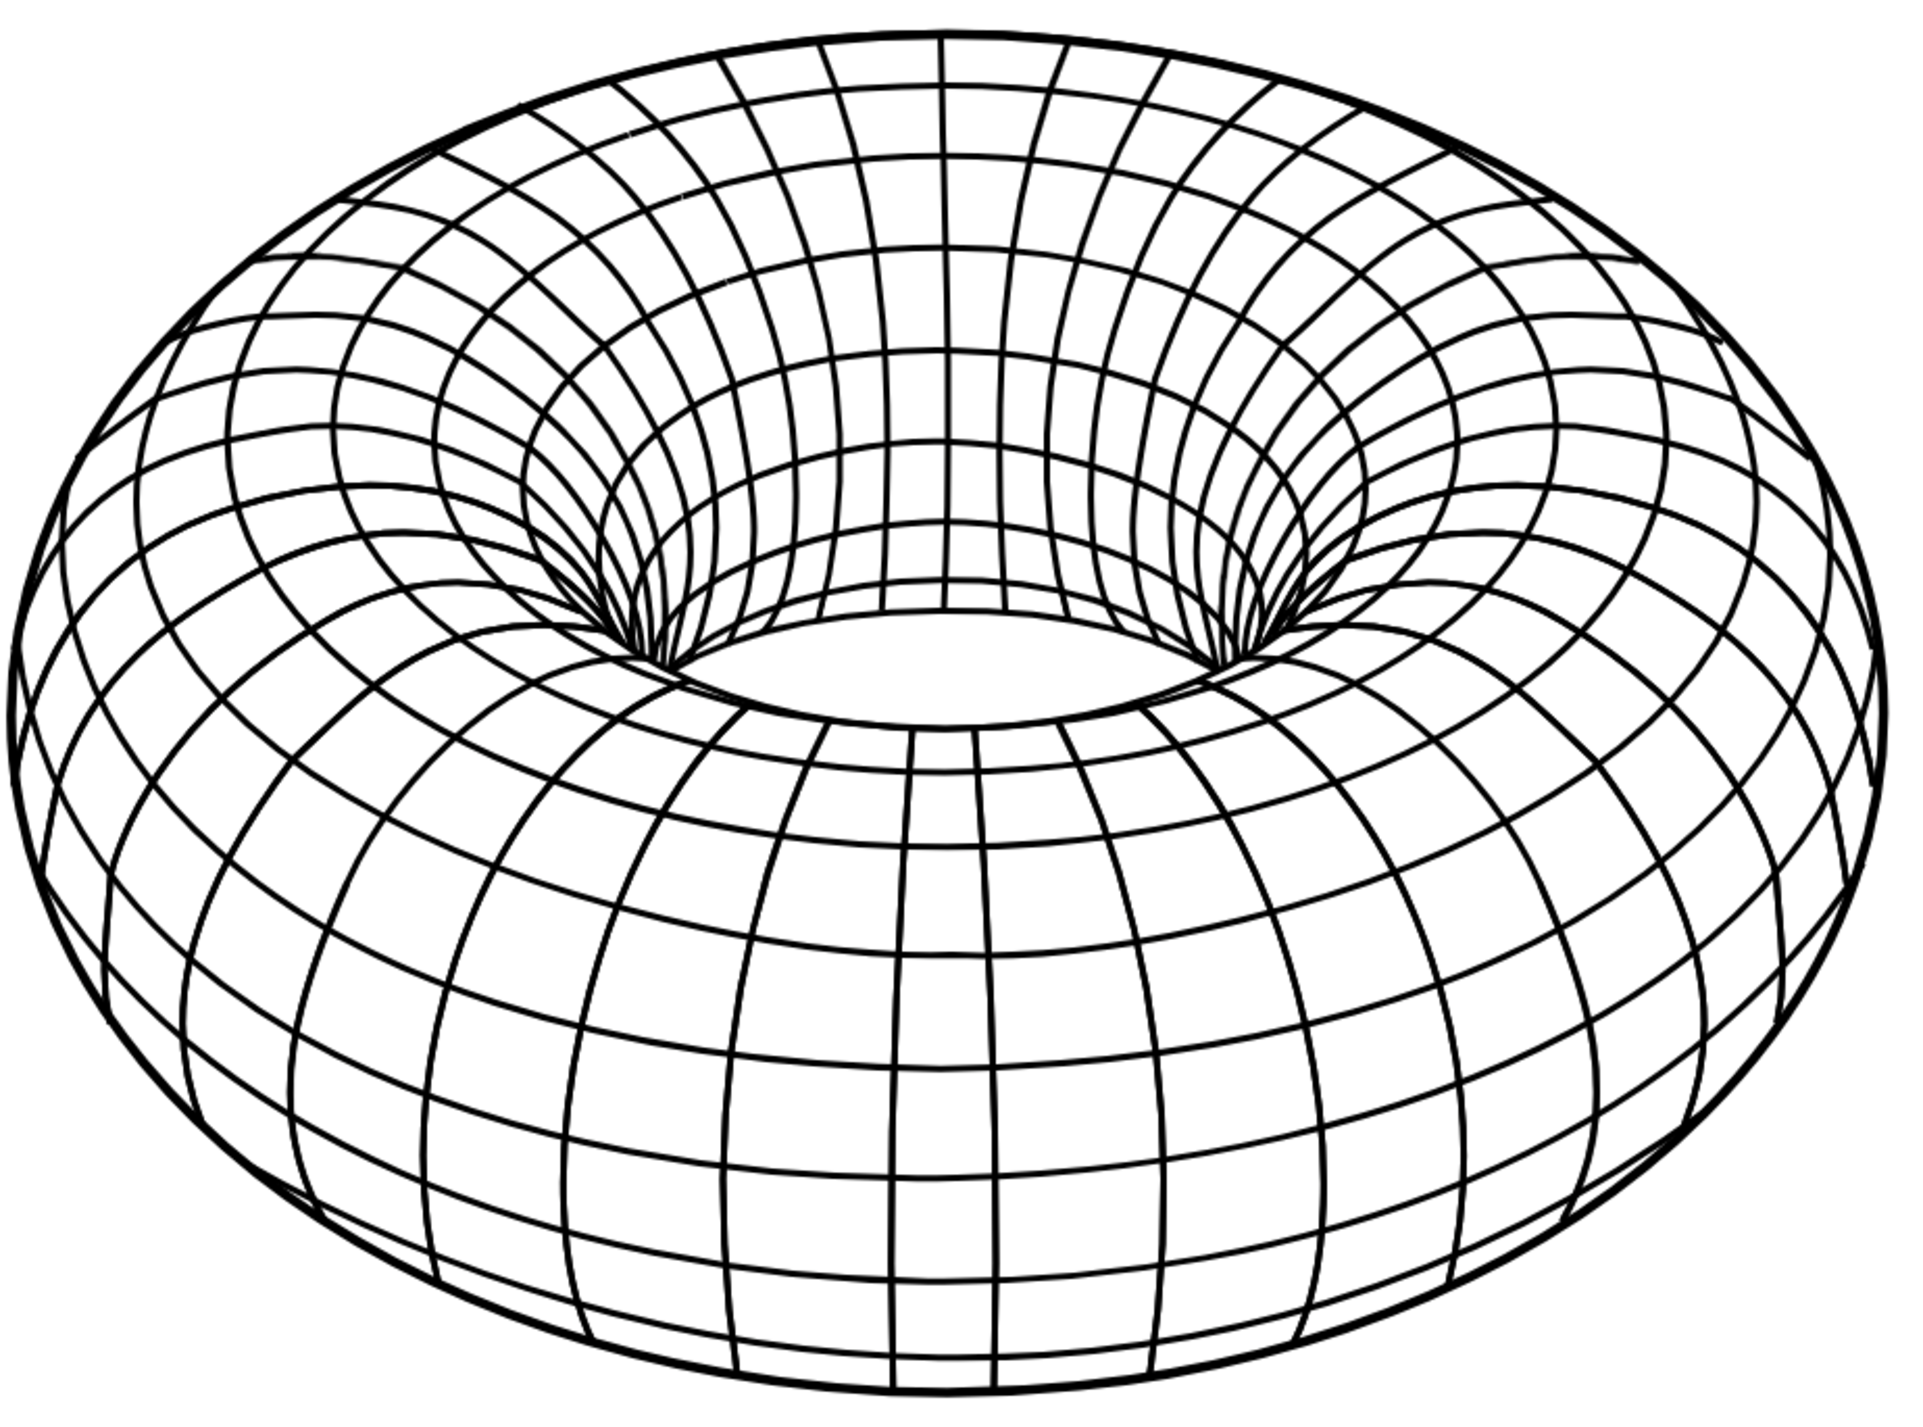
\includegraphics[width=0.45\textwidth]{torus.pdf}};
				\draw[->, very thick] (2.5,0) -- node[pos=1.4] {$y$} (3.2,
				0);	
				\draw[->, very thick] (0,0) -- node[pos=1.1] {$z$} (0,
				2.5);
				\draw[->, very thick] (-0.9, -0.9*4/3) -- node[pos=1.2]
				{$x$} (-1.5, -2);
			\end{tikzpicture}
		\] 
		Om te wys dat $M$ 'n hipervlak is, moet ons eers $\nabla f$ by 'n
		algemene punt $\ve{r} = (x,y,z) \in \mathbb{R}^3$ bereken:
		\[
			\nabla_\ve{r} f = \left( \frac{2x(2 - \sqrt{x^2 +
			y^2)}}{\sqrt{x^2 + y^2}}, \, \frac{2y(2 - \sqrt{x^2 +
			y^2)}}{\sqrt{x^2 + y^2}}, \, 2z \right)
		\]
		Let daarop dat $\nabla f$ nie \emph{oral} in $\mathbb{R}^3$
		bestaan nie, aangesien daar 'n probleem is as $x^2 + y^2 = 0$
		(d.w.s. op die $z$-as). Maar vir 'n punt $\ve{p} = (a, b, c)$ op
		$M$, kan ons nie $a^2 + b^2 = 0$ kry nie, aangesien dit volgens die
		vergelyking vir $M$ sou impliseer dat
		\[
			(2 - \sqrt{0})^2 + c^2 - 1 = 0,
		\]
		met ander woord, $c^2 = -3$, wat onmoontlik is. So $\nabla_\ve{p}
		f$ bestaan oral op $M$. Verder, veronderstel $\nabla_\ve{p} f =
		(0,0,0)$ en $\ve{p}$ l{\^e} op $M$. Dan, onder andere, is $2c = 0$
		so $c=0$, en daarom, volgens die vergelyking vir $M$, 
		\[
			(2 - \sqrt{a^2 + b^2})^2 = 1,
		\]
		wat impliseer dat $a$ en $b$ nie albei nul kan wees nie. Dit is 'n
		teenstelling, daarom is $\nabla_\ve{p} \neq \ve{0}$ oral op $M$.
		So $M$ is 'n hipervlak.
	\end{solution}
\end{example}

\begin{definition} Laat $M \subset \mathbb{R}^{n+1}$ 'n hipervlak
	geassosieer met 'n funksie $f : \mathbb{R}^{n+1} \rightarrow
	\mathbb{R}$ wees. Die \emph{raakruimte} van $M$ at $\ve{p} \in M$
	is:
	\[
		T_\ve{p} M := \{ \ve{v} \in \mathbb{R}^{n+1} \, : \, \nabla_\ve{p}
		f \dotp \ve{v} = 0 \}
	\]
\end{definition}
\begin{ramanujansays} Uit Meerveranderlike Calculus, weet ons dat ons die
	raakruimte van $M$ by $p$ soos volg kan uitdruk:
	\begin{align*}
		T_\ve{p} M &=  \{ \ve{v} \in \mathbb{R}^{n+1} \, : \, D_\ve{v} f
		(\ve{p}) = 0 \} \\
		&=  \left\{ \ve{v} \in \mathbb{R}^{n+1} \, : \,
		\frac{d}{dt}\Big|_{t=0} f(\ve{p} + t \ve{v}) = 0 \right\} 
	\end{align*}
\end{ramanujansays}

\begin{lemma} As $M$ ....

\end{lemma}

\begin{example} Bereken 'n basis vir die raakruimte aan die hiperbool $M$
	in Voorbeeld \ref{hyperbola_example} by $\ve{p} = (1, \sqrt{2})$. Teken
	'n prentjie om die resultaat te illustreer.
	\begin{solution}
		Ons het reeds die gradi(\"e)nt van $f$ by 'n punt $\ve{p} = (a,b)
		\in M$ bereken:
		\[
			\nabla_\ve{p} = (2b, -2a) \quad \mbox{ where $b^2 = 1 + a^2$}.
		\]
		Gevolglik het ons by $\ve{p} = (1, \sqrt{2})$ dat
		\[
			\nabla_\ve{p} f = (2 \sqrt{2}, -2).
		\] 
		Daarom 
		\begin{align*}
			T_\ve{p} M &= \{ (v_1, v_2) \in \mathbb{R}^2 : \nabla_\ve{p} f
			\dotp (v_1, v_2) = 0 \}  \\
			&= \{ (v_1, v_2) \in \mathbb{R}^2 : 2 \sqrt{2} v_1 - 2v_2 = 0
			\}
		\end{align*}
		'n Basis vir $T_\ve{p} M$ is $\ve{u} = (1, \frac{1}{\sqrt{2}})$.
		Die visualisering is:
		\[
			\begin{tikzpicture}[domain=-1.4:1.4]
				\draw[<->] (-2,0) -- (2,0) node[below] {$x$};
				\draw[<->] (0, -2) -- (0,2) node[right] {$y$};
				\draw[very thick] plot[id=p]  ({sinh(\x)}, {cosh(\x)});
				\draw[very thick] plot[id=p]  ({sinh(\x)}, {-cosh(\x)});
				\draw[very thick, red] plot[id=p] ({1.5*\x},
				{1/sqrt(2)*(1.5*\x) + (sqrt(2)-1/sqrt(2))}); 
				\draw[very thick, fill] (1, 1.414) circle (1pt) node[below
				right] {$\ve{p}$};
				\node at (-1.5, 1.4) {$M$};
				\draw[line width=0.5mm, blue, ->] (1, 1.414) -- (1.5, 1.414
				+ 0.5*0.707) node[below right] {$\ve{u}$};
			\end{tikzpicture}
		\qquad
		\begin{tikzpicture}[domain=-1.4:1.4]
			\draw[<->] (-2,0) -- (2,0) node[below] {$v_1$};
			\draw[<->] (0, -2) -- (0,2) node[right] {$v_2$};
			\draw[very thick, red] plot[id=p] ({1.5*\x},
			{1/sqrt(2)*(1.5*\x)});
			\node[red] at (2, 1.8) {$T_\ve{p} M$};
			\draw[line width=0.5mm, blue, ->] (0,0) -- (0.5, 0.5*0.707)
			node[right, yshift=-2pt] {$\ve{u}$};
		\end{tikzpicture}
		\]
		\begin{ramanujansays} Die rooi lyn in die eerste beeld, wat vir
			illustrasiedoeleindes geteken is, is die raakruimte wat
			geskuif is sodat dit deur $\ve{p}$ loop. Die ware raakruimte
			$T_\ve{p} M$ loop deur die oorsprong soos in die tweede beeld.
		\end{ramanujansays}

	\end{solution}
\end{example}





\end{appendices}



\backmatter
% bibliography, glossary and index would go here.

\end{document}
\grid
\grid
